% Formatvorlage f�r studentische Arbeiten der Arbeitsgruppe Software Systems
% Engineering am Institut f�r Informatik der Universit�t Hildesheim
%   erstellt von Christopher Voges, 28.04.2016
%   �berarbeitet von Sascha El-Sharkawy, 06.08.2019
%   https://sse.uni-hildesheim.de/studium-lehre/richtlinien-fuer-ausarbeitungen/vorlagen/

% Dokumentenkopf 
\documentclass[
    11pt, % Schriftgr��e
    DIV=10,
    ngerman, % f�r Umlaute, Silbentrennung etc.
    a4paper, % Papierformat
    twoside, % weiseitiges Dokument
    titlepage, % es wird eine Titelseite verwendet
    parskip=half, % Abstand zwischen Abs�tzen (halbe Zeile)
    headings=normal, % Gr��e der �berschriften verkleinern
    listof=totoc, % Verzeichnisse im Inhaltsverzeichnis auff�hren
    bibliography=totoc, % Literaturverzeichnis im Inhaltsverzeichnis auff�hren
    index=totoc, % Index im Inhaltsverzeichnis auff�hren
    captions=tableheading, % Beschriftung von Tabellen unterhalb ausgeben
		numbers=noenddot,
    final, % Status des Dokuments (final/draft)
]{scrreprt}

% Einbinden der Packages
% Entfernt Probleme durch Verwendung von Koma-Script Klassen (scrreport)
\usepackage{scrhack}
% Erlaubt Konfiguration von Header & Footer
\usepackage[automark,headsepline,footsepline,plainheadsepline,plainfootsepline]{scrlayer-scrpage}

% Anpassung an Sprache (deutsch)
\usepackage[ngerman]{babel}

% Umlaute
\usepackage[latin1]{inputenc}
\usepackage[T1]{fontenc}
\usepackage{textcomp} % Euro-Zeichen etc.

% Schrift
\usepackage{lmodern}
\usepackage{relsize}

% Einbinden von JPG-Grafiken erm�glichen
\usepackage[dvips,final]{graphicx}

% Erm�glichen mathematischer Symbole
\usepackage{amsmath,amsfonts}

% F�r die Definition der Zeilenabst�nde, Seitenr�nder etc.
\usepackage{setspace}
\usepackage{geometry}

% URL-Unterst�tzung
\usepackage{url}

\usepackage{float}

% Abk�rzungsverzeichnis 
% Alles weitere hierzu in: "Inhalt\Abkuerzungen.tex".
\usepackage[intoc]{nomencl}
\let\abbrev\nomenclature
\renewcommand{\nomname}{Abk�rzungsverzeichnis}
\setlength{\nomlabelwidth}{.15\textwidth}

% PDF-Optionen -----------------------------------------------------------------
\usepackage[
    bookmarks, % Es werden Bookmarks verwendet
    bookmarksopen=true, % Farbe von Bookmarks
    colorlinks=true, % Farbe von Verkn�pfungen
    linkcolor=black, % einfache interne Verkn�pfungen
    anchorcolor=black, % Ankertext
    citecolor=black, % Verweise auf Literaturverzeichniseintr�ge im Text
    filecolor=black, % Verkn�pfungen, die lokale Dateien �ffnen
    menucolor=black, % Acrobat-Men�punkte
    urlcolor=black, % Farbe der URLs
    plainpages=false, % zur korrekten Erstellung der Bookmarks
    pdfpagelabels, % zur korrekten Erstellung der Bookmarks
    hypertexnames=false, % zur korrekten Erstellung der Bookmarks
    linktocpage, % Seitenzahlen anstatt Text im Inhaltsverzeichnis verlinken
    pdfusetitle % Erm�glicht das Setzen der Meta-Daten des erzeugten PDFs
]{hyperref}
% \renewcommand{\theHsection}{\thepart.section.\thesection}
% \hypersetup{
%     %pdftitle={\titel \untertitel},
%     pdfauthor={\autor},
%     pdfcreator={\autor}
%     %pdfsubject={\titel \untertitel},
%    % pdfkeywords={\titel \untertitel}
% }

% Wird f�r Teile der Formatierung des Deckblatts und die Verwendung von
% Aufz�hlungen ben�tigt
\usepackage{listings}
\usepackage{xcolor} 
\usepackage{tabularx}


% fortlaufendes Durchnummerieren der Fu�noten
\usepackage{chngcntr}

% bei der Definition eigener Befehle ben�tigt
\usepackage{ifthen}

% sorgt daf�r, dass Leerzeichen hinter parameterlosen Makros nicht als Makroendezeichen interpretiert werden
\usepackage{xspace}

% F�r das Erstellen eines Glossars
\usepackage[toc, automake, nonumberlist]{glossaries}

\usepackage[figure,table,lstlisting]{totalcount}

% Einbinden der Meta-Informationen
% Meta-Informationen 
% Falls Umlaute oder ein *�* vorkommen:
\usepackage[latin1]{inputenc}
\usepackage{babel}
\usepackage[T1]{fontenc}
\usepackage{graphicx}
\usepackage{pdfpages}
% Hier k�nnen Sie Informationen zur Arbeit, sich selbst und Ihren Betreuern
% hinterlegen.
\newcommand{\titel}{Die Entwicklung eines rundenbasierten Strategiespiels, das es KI-Spielern erm�glicht gegeneinander anzutreten und KIs gegeneinander zu testen} % Name der Arbeit
\newcommand{\untertitel}{Eine beispielhafte Umsetzung in Form von Siedler von Catan} % Optional mit Untertitil
% Art der Arbeit ggf. zus�tzlich der Titel der Veranstaltung
\newcommand{\art}{Bachelor} 
\newcommand{\studiengang}{Bachelor of Science (B.\,Sc.) in Informationsmanagement und Informationstechnologie (IMIT)} % Ihr Studiengang
\newcommand{\autor}{Tjark Harjes} % Ihr Name
\newcommand{\email}{harjes@uni-hildesheim.de}% Ihre aktuelle und g�ltige E-Mail-Adresse
\newcommand{\matnr}{301249} % Ihre Matrikelnummer

% Die Angaben zu uns:
\newcommand{\institut}{Institut f�r Betriebwirtschaft}
\newcommand{\arbeitsgruppe}{Projektarbeit}
\newcommand{\erstgutachter}{Prof. Dr. Klaus-Dieter Althoff}% Ihr(e) Erstgutachter
\newcommand{\zweitgutachter}{Pascal Reuss, M.Sc.}% Ihr(e) Zweitgutachter
\newcommand{\universitaet}{Universit�t Hildesheim\ \textbullet \ Universit�tsplatz 1 \ \textbullet \ D-31134 Hildesheim}
\newcommand{\adresse}{\arbeitsgruppe \ \textbullet \ \institut \\ \universitaet}

\newcommand{\version}{Version 1.0}% Die Version der Arbeit

\newcommand{\quotes}[1]{``#1''}

\newcommand{\equationsBig}{
	\scalebox{2}{$\BODY$}
}

% Wird 'projektarbeit' auf 'true' gesetzt, wird keine Eigenst�ndigkeitserkl�rung
% erzeugt.
\newboolean{projektarbeit}
\setboolean{projektarbeit}{true}

% Wird 'final' auf 'true' gesetzt, werden folgende �nderungen vorgenommen:
% -Entfernen von Datum in der Kopf- und Versionsnummer in der Fu�zeile
% -Entfernen von Datum und Versionsnummer vom Deckblatt
% -Es werden Leerseiten f�r den doppelseitigen Druck eingef�gt
\newboolean{final}
\setboolean{final}{true}





% Erstellung der Verzeichnisse und Glossars aktivieren
\makeindex
\makenomenclature
\makeglossaries 
\glstoctrue 


% Kopf- und Fu�zeilen, Seitenr�nder etc. anpassen
% Zeilenabstand: einfach 
\newcommand{\zeilenabstandHauptteil}{1.0}
\newcommand{\zeilenabstandAnhang}{1.0}

% Seitenr�nder
\setlength{\topskip}{\ht\strutbox} % behebt Warnung von geometry
% Initiales Papierformat, wird nach dem Deckblatt teilwiese ge�ndert 
\geometry{paper=a4paper,left=3.5cm, right=2.5cm, top=2.5cm, bottom=2.9cm, headsep=.6cm}

%% Einstellen der Schriftgr��en der �berschriften
\setkomafont{chapter}{\LARGE\bfseries\rmfamily}
\setkomafont{section}{\Large\bfseries\rmfamily}
\setkomafont{subsection}{\large\bfseries\rmfamily}
\setkomafont{subsubsection}{\large\mdseries\rmfamily}
\setkomafont{pageheadfoot}{\normalfont}

%% Einstellen der Abst�nde vor und nach den �berschriften
\RedeclareSectionCommand[
  %runin=false,
  afterindent=false,
  beforeskip=0pt,
  afterskip=.05\baselineskip]{chapter}
\RedeclareSectionCommand[
  %runin=false,
  afterindent=false,
  beforeskip=0pt,
  afterskip=.05\baselineskip]{section}
\RedeclareSectionCommand[
  %runin=false,
  afterindent=false,
  beforeskip=0pt,
  afterskip=.05\baselineskip]{subsection}
\RedeclareSectionCommand[
  %runin=false,
  afterindent=false,
  beforeskip=0pt,
  afterskip=.05\baselineskip]{subsubsection}

% Header & Footer konfigurieren
\renewcommand*{\chaptermarkformat}{} % Keine Nummerierung im Header
\clearpairofpagestyles % Voreinstellungen l�schen
% E = Even page  (Gerade Seitennummer)
% O = Odd page   (Ungerade Seitennummer)
% L = Left side	 (Linker Teil der Seite)
% C = Centered   (Mittlerer Teil der Seite)
% R = Right side (Rechter Teil der Seite)
% Auf ungeraden Seiten: Kapitel�berschrift, oben rechts
\rohead[\leftmark]{\leftmark}
% Auf geraden Seiten: Titel der Arbeit, oben links
\lehead[\titel]{\titel}
% Seitenzahlen in der Mitte eines Zweiseitigenausdrucks
\rofoot[\thepage]{\thepage}
\lefoot[\thepage]{\thepage}

\ifthenelse{\boolean{final}}{% Keine besondere Aktion in der finalen Fassung
  } {
		%Versionsnummer f�r Draft
		\lohead[Version vom \today~(Vor Abgabe entfernen)]{Version vom \today~(Vor Abgabe entfernen)}
		\rehead[Version vom \today~(Vor Abgabe entfernen)]{Version vom \today~(Vor Abgabe entfernen)}
		\lofoot[Version vom \version~(Vor Abgabe entfernen)]{Version vom \version~(Vor Abgabe entfernen)}
		\refoot[Version vom \version~(Vor Abgabe entfernen)]{Version vom \version~(Vor Abgabe entfernen)}
	}

% erzeugt ein wenig mehr Platz hinter einem Punkt
\frenchspacing 

% Schusterjungen und Hurenkinder vermeiden
\clubpenalty = 10000
\widowpenalty = 10000 
\displaywidowpenalty = 10000

% Quellcode-Ausgabe formatieren
\lstset{numbers=left, numberstyle=\tiny, numbersep=5pt, breaklines=true}
\lstset{emph={square}, emphstyle=\color{red}, emph={[2]root,base}, emphstyle={[2]\color{blue}}}

% Fu�noten fortlaufend durchnummerieren
\counterwithout{footnote}{chapter}

% Einstellungen f�r Listings
\definecolor{hellgelb}{rgb}{1,1,0.9}
\definecolor{colKeys}{rgb}{0,0,1}
\definecolor{colIdentifier}{rgb}{0,0,0}
\definecolor{colComments}{rgb}{1,0,0}
\definecolor{colString}{rgb}{0,0.5,0}
\lstset{
    float=hbp,
    columns=flexible,
    tabsize=2,
    frame=single,
    extendedchars=true,
    showspaces=false,
    showstringspaces=false,
    numbers=left,
    numberstyle=\tiny,
    breaklines=true,
    breakautoindent=true,
    xleftmargin=0.6cm,
    xrightmargin=0.1cm,
    captionpos=b
}

% Eigene Definitionen f�r Silbentrennung laden
% Trennvorschl�ge im Text werden mit \" angegeben
% untrennbare W�rter und Ausnahmen von der normalen Trennung k�nnen in dieser
% Datei mittels \hyphenation definiert werden


% Eigene LaTeX-Befehle laden
% Eigene Befehle, z.B.:
\newcommand{\fett}[1]{\textbf{#1}}

% Hier beginnt das eigentliche Dokument
\begin{document}
\title{\titel}
\author{\autor}

% Setzt wie tief Abschnitte numeriert und ins Inhaltsverzeichnis
% aufgenommen werden sollen, hier: bis inkl. SubSubSection (z.B. 1.1.1.1).
\setcounter{secnumdepth}{3}
\setcounter{tocdepth}{3}

% Deckblatt einbinden
% Erzeugt das Deckblatt
%   Bei zu langem Arbeitstitel m�ssen die vertikalen Abst�nde (\vspace)
%   angepasst werden, damit das Deckblatt weiterhin auf eine Seite passt.
\begin{titlepage}
\newgeometry{top=2cm,bottom=2cm,left=2cm,right=2cm}
\begin{flushleft}
	%\includegraphics[width=6.75cm]{Abbildungen/luh_logo.ps}\\
	{\Large Universit"at Hildesheim \\
		\large Institut f"ur Informatik} \\
	\begin{flushright}\vspace*{-5cm}
		
\includegraphics[scale=0.087]{uni_hi_logo.pdf}
	\end{flushright}
\end{flushleft}

\begin{center}
	\vspace{3cm}
	\Huge{\textbf{\titel}}
\end{center}
\begin{center}
    \vspace*{3cm}
    \large{\textbf{\art~im Studiengang \studiengang}}\\
    Sommersemester 2020
    \vspace{1cm}
\end{center}
\begin{center}
vorgelegt von \\[1.5ex] 
\textbf{Tjark Harjes} \\[1.5ex]
Matr.-Nr.: 301249 \\
4. Semester IMIT \\
E-Mail: harjes@uni-hildesheim.de\\[1.5cm]
Hildesheim, den \textbf{07.06.2020} \\ 
\end{center} 
\begin{flushleft}
	\vspace{4cm}
	\textbf{Erstgutachter: } \erstgutachter \\
	\textbf{Zweitgutachter: } \zweitgutachter
\end{flushleft}
\end{titlepage}
\restoregeometry

% Setzen des Papierformats f�r den Rest des Dokuments
%\newgeometry{left=3.5cm, right=2.5cm, top=2.9cm, bottom=2.9cm}

% Bei finaler Fassung: Leere Seite als R�ckseite des Deckblatts 
%\ifthenelse{\boolean{final}}{\cleardoublepage}{} 

% Selbstst�ndigkeitserkl�rung einbinden
\ifthenelse{\boolean{projektarbeit}}{}{\thispagestyle{empty}
\vspace*{.5cm}
\Large \textbf{Eigenst�ndigkeitserkl�rung} \normalsize
\begin{verbatim}
\end{verbatim}\setstretch{1.20}
% Bei abweichender Vorgabe bspw. durch Ihr Pr�fungsordnung, muss der
% nachfolgende Text durch den vorgegeben ersetzt werden!
\fett{Erkl�rung �ber das selbstst�ndige Verfassen von "\titel"}

Ich versichere hiermit, dass ich die vorstehende Arbeit selbstst�ndig verfasst
und keine anderen als die angegebenen Hilfsmittel benutzt habe. Die Stellen der obigen Arbeit, die anderen Werken dem Wortlaut oder dem Sinn nach entnommen wurden, habe ich in jedem Fall durch die Angabe der Quelle bzw. der Herkunft, auch der benutzten Sekund�rliteratur, als Entlehnung kenntlich gemacht. Dies gilt auch f�r Zeichnungen, Skizzen, bildliche Darstellungen sowie f�r Quellen aus dem Internet und anderen elektronischen Text- und Datensammlungen und dergleichen. Die eingereichte Arbeit ist nicht anderweitig als Pr�fungsleistung verwendet worden oder in deutscher oder einer anderen Sprache als Ver�ffentlichung erschienen. Mir ist bewusst, dass wahrheitswidrige Angaben als T�uschung behandelt werden.

Hildesheim, den~\today

\unitlength 5mm
\begin{picture}(5,4) \put(0,0) {\line(1,0){22}} \end{picture}\\
\autor
}

% Bei finaler Fassung: Leere Seite als R�ckseite der Erkl�rung
\ifthenelse{\boolean{projektarbeit}}{}{\ifthenelse{\boolean{final}}{\cleardoublepage}{}}

% Abstract einbinden
%% Vor dem Hauptteil werden die Seiten in gro�en r�mischen Ziffern nummeriert.
\pagenumbering{roman}

\section*{Kurzfassung}
\label{sec:Kurzfassung}
Die folgende Projektarbeit befasst sich mit der Studienplatzvergabe indischer Hochschulen. Diese unterlag lange Zeit einem Problem: Es gab deutlich mehr Bewerber als Pl�tze und dennoch blieben viele dieser Pl�tze unbesetzt. Ziel ist es daher dem Leser einen Einblick in die Studienplatzvergabe Indiens zu geben und  anhand des L�sungsvorschlages von (vgl. \cite[S. 1ff]{Baswana2015}) Probleme dieser darzustellen. Zudem soll das Verfahren implementiert, sowie ein Vergleich zu verschiedenen Alternativen gezogen werden. Auf dieser Grundlage wurden drei Forschungsfragen formuliert: \\

\fett{RQ1:} Wie wird versucht, die Herausforderungen der Studienplatzvergabe in Indien zu bew�ltigen?\\
\fett{RQ2:} Wie kann das vorgestellte Verfahren implementiert werden? \\
\fett{RQ3:} Welche Alternativen Ans�tze existieren zur L�sung des Problems der Platzvergabe an Hochschulen?\\

\fett{Resultat der Arbeit:} Das gezeigte Verfahren erf�llt alle gestellten Anforderungen und ist in der Lage die frei bleibenden Pl�tze um ca. 70\% zu reduzieren. Dennoch existieren Verbesserungsm�glichkeiten, die zum Teil aus den Alternativen hervorgehen. Generell k�nnen aber auch Schl�sse in Bezug auf Quotenregelungen und allgemein Sitzplatzvergabe aus dem Verfahren gewonnen werden. Die Implementierung ist trotz der Vielzahl der Anforderungen nicht komplexer als f�r vergleichbare Algorithmen.




% Bei finaler Fassung: Leere Seite als R�ckseite des Abstracts
%\ifthenelse{\boolean{final}}{\cleardoublepage}{}

\pagenumbering{roman}
% Verzeichnisse drucken
\tableofcontents% Inhaltsverzeichnis

% Glossar einbinden
% Ein Beispiel f�r einen Glossareintrag
% Nur Eintr�ge, die mindestens ein Mal referenziert wurden 
% (z.B.: \gls{computer}), tauchen im Glossar am Ende der Arbeit auf.
\newglossaryentry{abk:API} {
	name=API,
	description={Application-Program-Interface}
}
\newglossaryentry{abk:JSON} {
	name=JSON,
	description={JavaScript Object Notation}
}
\newglossaryentry{abk:KI} {
	name=KI,
	description={K�nstliche Intelligenz}
}
\newglossaryentry{abk:WBS} {
	name=WBS,
	description={Wissensbasiertes System}
}
\label{sec:Glossar}

% Mit diesem Befehl werden nach nicht referenierte Glossareintr�ge
% ausgegeben (Nur zum Testen einkommentieren!)
\glsaddall

% Glossar drucken
\printglossary[title=Abk�rzungsverzeichnis]
%\addcontentsline{toc}{chapter}{Abk�rzungsverzeichnis}

% Glossar drucken
%\printglossary[title=Abk�rzungsverzeichnis]
%\addcontentsline{toc}{chapter}{Abk�rzungsverzeichnis}

% Wenn Abbildungs- und Tabellenverzeichnis auf die selbe Seite sollen: 
\iftotalfigures\listoffigures\fi
\begingroup 
\let\clearpage\relax
\vspace{1cm} 
\iftotaltables\listoftables\fi
\endgroup
 
% Wenn Abbildungs- und Tabellenverzeichnis je auf einer eigenen Seite beginnen
% sollen: 
% \listoffigures % Abbildungsverzeichnis
% \listoftables % Tabellenverzeichnis
\renewcommand{\lstlistlistingname}{Quellcode-Verzeichnis}
\lstlistoflistings

\clearpage
% Abk�rzungsverzeichnis einbinden
%% 2 Beispiele f�r Abk�rzungen
\nomenclature{API}{Application Programming Interface}
\nomenclature{XML}{Extensible Markup Language}


% F�r korrekte �berschrift in der Kopfzeile
%\clearpage\markboth{\nomname}{\nomname}

% Drucken des Abk�rzungsverzeichnisses
%\printnomenclature
%\label{cha:Abkuerzungsverzeichnis}
 
% Arabische Seitenzahlen im Hauptteil 
%\ifthenelse{\boolean{final}}{\cleardoublepage}{\clearpage}

% Die Inhaltskapitel aus "Inhalt.tex" einbinden
\begin{spacing}{\zeilenabstandHauptteil}
\pagenumbering{arabic}
% Hier k�nnen die einzelnen Kapitel inkludiert werden. 
% Die Dateien m�ssen auf .tex enden. Diese Endung muss
% beim Inkludieren aber weggelassen werden.
% Info: \include und \input unterscheiden sich im wesentlichen darin, dass bei
% \include immer eine neue Seite angefangen wird.
\pagenumbering{arabic}
\chapter{Einleitung}
\label{cha:Einleitung}
K�nstliche Intelligenz (KI) ist heutzutage in Computerspielen weit verbreitet und fand schon Ende des letztes Jahrtausends Einzug in die Spieleindustrie (\cite[vgl. S. 1]{Davis1999}). Seitdem haben sich die KIs weiterentwickelt und agieren heute besser als damals. Dennoch ist die Entwicklung von starker KI f�r Strategiespiele aufwendig, weshalb h�ufig KIs gebaut werden, die durch das \quotes{Cheaten} einen Vorteil gegen�ber menschlichen Spielern haben (vgl. \cite[vgl. S. 24]{Ruiz2007}). 

In dieser Arbeit soll das bekannte Gesellschaftsspiel \textit{Siedler von Catan} als Computerspiel umgesetzt werden und durch KIs spielbar sein. Dabei werden an die KIs die gleichen Ma�st�be angelegt, die auch f�r menschliche Spieler gelten. Ferner wird ihnen das \quotes{Cheaten} nicht erlaubt.

\section{Ziel der Arbeit}
Ziel dieser Bachelorarbeit ist es, ein rundenbasiertes Strategiespiel f�r KI spielbar umzusetzen sowie die Konzeption, Implementation und Evaluation zu dokumentieren. Konkret wurde dabei das bekannte Gemeinschaftsspiel \textit{Siedler von Catan} als Ziel der Implementation gew�hlt. 

In dieser schriftlichen Ausarbeitung werden demnach alle theoretischen Aspekte der Software betrachtet, die dazu umgesetzt wurden. Es soll von den Grundlagen, die zum Verst�ndnis sp�terer Ausf�hrungen wichtig sind, bis zur Evaluation der entworfenen Software alles abgedeckt werden. 

\section{Aufbau der Arbeit}
Zun�chst werden in Kapitel 2 die n�tigen Grundlagen thematisiert, die zum Nachvollziehen sp�terer Kapitel n�tig sind. In Kapitel 3 wird dann auf die Konzeption der Software eingegangen. Hier wird wiederum zwischen einer Problemstellung, welche die Gr�nde und Ziele der Arbeit konkretisiert, und einem Entwurf f�r die Software unterschieden. 

Die Erl�uterung der tats�chlichen Implementation erfolgt anschlie�end im 4. Kapitel, welches im Detail auf alle wichtigen Bestandteile der angefertigten Software eingeht. In diesem Kapitel soll auch ein Vergleich zwischen dem Entwurf und der tats�chlichen Umsetzung erfolgen. 

Im 5. Kapitel soll dann schlie�lich zur Evaluation �bergegangen werden. Diese soll pr�fen, ob die gestellten Anforderungen erf�llt werden konnten und eine Bewertung des Implementierten vornehmen. Die Evaluation wird auf Grundlage der erf�llten bzw. nicht erf�llten Anforderungen und durchgef�hrten Tests vorgenommen. Nach der Bewertung werden Probleme der Entwicklung angebracht, sowie deren Ursachen zu beschrieben.

Nach der Evaluation folgt der Schlussteil in dem die Kernpunkte dieser Ausarbeitung zusammengefasst werden und ein Fazit gezogen wird. Au�erdem wird ein Ausblick gegeben, indem L�sungen zu den in Kapitel 5 beschriebenen Problemen pr�sentiert werden. Au�erdem werden weitere Ans�tze f�r Verbesserungen der Software untersucht. 





\chapter{Grundlagen}
Da diese Ausarbeitung die Entwicklung eines Strategiespiels f�r computergesteuerte Spieler behandelt, sollen in diesem Kapitel die Grundlagen eines solchen Spiels erl�utert werden. Dieses Kapitel ist insofern von besonderer Bedeutung, als dass der Entwurf und die darauf basierende Implementation des Spieles auf den hier dargestellten Grundlagen basieren. Ferner wird in der Evaluation des Spieles nochmals Bezug auf dieses genommen. \\

Die Entwicklung computergesteuerter Spieler reicht inzwischen schon �ber 20 Jahre zur�ck. So schrieben \cite[vgl. S. 24ff]{Davis1999} 1999 von ihren Entwicklungen, die beispielsweise in das bekannte Strategiespiel \textit{Civilization: Call To Power} Einzug fanden. Das ist u.a deshalb beeindruckend, weil der Sieg von Deep Blue �ber Garri Kasparow in Spiel Schach zu diesem Zeitpunkt erst 3 Jahre zur�ck lag. Seitdem hat sich sowohl f�r Echtzeitspiele als auch f�r rundenbasierte Spiele viel getan. Bis heute ist das einprogrammierte \quotes{Cheaten} der Computergegner ein Problem, was von \cite[vgl. S. 1]{Ruiz2007} n�her beschrieben wurde, wobei ein dieses Problem im Kontext dieser Arbeit nicht auftreten wird, da das Ziel dieser Arbeit nicht ist, eine m�glichst spannende KI zu erstellen. Die Arbeit von \cite{Ruiz2007} ist dennoch interessant, weil die Autoren sich speziell mit dem Case-Based-Reasoning auseinander gesetzt haben. Sie pr�sentieren zudem eine Idee f�r die Interaktion von Spiel und Spieler mittels einer \textit{Application Programming Interface} (API). Die API sei in der Lage, eine Verbindung zwischen der KI und dem Spiel zu schaffen, sodass die KI Zugriff auf alle Informationen habe und gleichzeitig Anweisungen erteilen k�nne. Diese API ist vonn�ten, da eine Konvertierung der auf dem Bildschirm erscheinenden Informationen erfolgen muss, um diese f�r einen Computer wieder verarbeitbar zu machen. Diese entsprechende Architektur l�sst sich, wie in Abb. \ref{fig:Architektur} zu sehen ist, oberfl�chlich darstellen. \\

\begin{figure}[h]
	\centering
	
\includegraphics[height=9cm]{Bilder/Architektur.png}
	\caption{Architektur eines KI-Spiels (In Anlehnung an \cite[vgl. S. 4]{Ruiz2007})}
	\label{fig:Architektur}
\end{figure}

Abb. \ref{fig:Architektur} zeigt drei Komponenten, die �ber vier Pfeile miteinander verbunden sind. Die oberste Komponente repr�sentiert die KI. Sie steht nicht etwa f�r den Spieler, der im Spiel zu sehen ist, sondern nur f�r die dahinter stehende Logik - So wie ein menschlicher Spieler auch nicht die Figur im Spiel ist, sondern diese Figur nur eine Repr�sentation seiner selbst darstellt. Auf gleiche Weise funktioniert dieses Prinzip auch mit einem computergesteuertem Spieler. Er erh�lt Informationen und erteilt Anweisungen �ber eine geeignete Schnittstelle (hier: die API) und wird im Spiel ohne eine andere Verk�rperung durch eine Spielfigur verbildlicht. \\

Die unterste Komponente stellt das Spiel dar. Zwischen der KI- und der Spielkomponente befindet sich die API-Komponente. Diese ist die erw�hnte Schnittstelle und erm�glicht eine Kommunikation zwischen dem Spiel und den KI-Spielern. Das Spiel kann �ber die API Informationen an einen Spieler senden und dem Spieler wird so das Erhalten von Informationen erm�glicht. �quivalent dazu funktioniert das Senden und Empfangen von Anweisungen.Diesmal sendet jedoch der Spieler die Anweisungen ab, w�hrend das Spiel diese empf�ngt und ggf. verarbeitet. So wird dem Spieler die Steuerung seiner Repr�sentation im Spiel erm�glicht, unabh�ngig davon, ob es sich um eine Figur oder ein Reich oder �hnliches handelt. \\

\begin{figure}[h]
	\centering
	
\includegraphics[height=9cm]{Bilder/Architektur-analog-mensch.png}
	\caption{Architektur menschlicher Spieler (eigene Darstellung)}
	\label{fig:Architektur_menschlich}
\end{figure}

Abbildung \ref{fig:Architektur_menschlich} zeigt eine analoge Darstellung der Komponenten f�r menschliche Spieler. Diesmal stellt die oberste Komponente nicht etwa den KI-Spieler dar, sondern einen menschlichen Spieler. Und auch die mittlere Komponente ist eine andere. Zuvor wurde die Mitte durch die API veranschaulicht. Jetzt sind stattdessen zwei Komponenten zu sehen: \textit{Bildschirm/Grafik} und \textit{Tastatur/Maus}. Nur die untere Komponente \textit{Spiel} �ndert sich nicht. Diese Abbildung soll die Parallelen zwischen der Verwendung eines KI-Spielers und der eines menschlichen Spielers weiter verdeutlichen, denn ob ein Mensch oder eine Maschine spielt, ist im Prinzip das Gleiche. Wichtig ist nur die Umsetzung der Schnittstelle und da meist ein Mensch das Spiel spielt, erscheinen Maus, Tastatur und Bildschirm als Schnittstelle intuitiver. Doch die Aufnahme von Informationen �ber einen Bildschirm und das Erteilen von Anweisungen mit Maus und Tastatur ist nichts anderes als das Verwenden einer Schnittstelle zum Steuern der eigenen Repr�sentation im Spiel. F�r die KI wird das Gleiche erreicht, wenn sie Informationen und Anweisungen �ber eine API erh�lt bzw. versendet. \\

Das beschriebene Prinzip gilt also nicht exklusiv f�r computergesteuerte Gegner. Anhand von Abb. \ref{fig:Architektur_menschlich} wird deutlich, dass es sich viel allgemeiner um einen Standardweg der Kommunikation zwischen einem Programm und einer nicht darin enthaltenen Entit�t handelt. \\

\section{Computergegner in rundenbasierten Strategiespielen}
Nachdem im obigen Abschnitt allgemein auf die Interaktion zwischen Spielern und dem Spiel eingegangen wurde, sollen im Folgenden ein m�glicher Aufbau und die Konzeption von Computergegnern beschrieben werden. \\

Ein KI-Spieler kann auf unterschiedliche Weisen konzipiert werden. So ist es m�glich, feste Strategien von Hand zu implementieren und diese den Spieler ausf�hren zu lassen. Des Weiteren k�nnen KIs durch Neuronale Netze und dem damit verbundenem Deep Learning realisiert werden \cite[vgl. S. 1]{Mayer2007}. AAu�erdem ist es m�glich, KI-Spieler zu entwickeln, die ihre Strategien mithilfe Wissensbasierter Systeme (WBS) umsetzen. \cite[vgl. S.5]{Ruiz2007}. Alle diese Varianten k�nnen gute Ergebnisse erzielen und ihre Einsatz h�ngt ma�geblich vom gew�nschten Ziel ab: so w�rde eine von Hand programmierte KI dann zum Einsatz kommen, wenn nicht unbedingt die bestm�gliche Performance gew�nscht ist, aber stattdessen ein ganz bestimmtes Verhalten erzeugt werden soll. Ein Ziel, das beispielsweise durch Neuronale Netze nur schwer zu erreichen w�re. Wenn andererseits die st�rkste m�gliche KI als Ergebnis herauskommen soll, dann eignen sich Herangehensweisen, die die KIs ihre eigenen Methoden finden lassen und durch Lernprozesse auf diesem Wege die besten Strategien ausmachen kann. Dies ist etwas, was bei hart-kodierten Spielern wiederum �u�ert schwer, wenn �berhaupt zu erreichen ist. \\

\subsection{Der KI-Spieler als Wissensbasiertes System}
\label{sec:WBS}
Da das Produkt dieser Arbeit jedoch haupts�chlich f�r den Einsatz von KI-Spielern nach dem Prinzip der WBS gebraucht werden soll, wird der Fokus der Erl�uterungen auf diesen liegen. Abbildung \ref{fig:WBS} zeigt, wie ein WBS grundlegend aufgebaut ist. Es wird deutlich, dass eine Abgrenzung zwischen dem Interpreter und dem Wissen gezogen wird. Das ist einer der identifizierenden Punkte eines solchen Systems, da die Handlungen des Systems sind nicht nur vom Interpreter an sich abh�ngig sondern auch von der dahinter liegenden Wissensbasis. \\
Das Konzept des Systems l�sst sich auch anhand der Abbildung erkennen. Zun�chst erfolgt eine Eingabe, die dieser Interpreter wahrnimmt. Anschlie�end greift dieser zur Verarbeitung der Eingabe auf die angeschlossene Wissensbasis zur�ck und versucht, mit Hilfe dieser eine passende L�sung auf die Problemstellung zu finden. Schlussendlich wird die L�sung als Ausgabe zur�ckgeliefert. Bezogen auf eine KI im Kontext eines Videospiels sind die Eingaben als Informationen, die das Spiel liefert, zu verstehen. Man denke hierbei an Abb. \ref{fig:Architektur} zur�ck, bei der die KI ihre Informationen �ber die API erhalten hat. Diese Informationen sind demnach die Eingabe f�r das System. In der gleichen Abbildung wurde auch gezeigt, dass es sich bei der Ausgabe der KI um Anweisungen handelt. Demnach gibt auch das WBS in diesem Fall Anweisungen als Ausgabe zur�ck. Also muss durch den Interpreter eine Art Konvertierung einer Information in eine Handlung erfolgen, die von der Repr�sentation des Spielers im Spiel ausgef�hrt werden kann. Hierbei ist dennoch zu beachten, dass nicht jede gesendete Information auch eine direkte Anweisung zur Folge haben muss. Die Informationen dienen vielmehr der Findung einer Strategie durch den Interpreter und der Interpreter, wobei dieser Aktionen der gefundenen Strategie auch dann ausf�hren lassen kann, wenn gerade gar kein Input erfolgt ist.\\
In Bezug auf die Fallbasis ist wichtig zu wissen, dass diese sowohl Wissen �ber das Spiel und die m�glichen Strategien, als auch Wissen �ber das eigene System enth�lt. 

\begin{figure}[h]
	\centering
	
\includegraphics[width=12cm]{Bilder/WissensbasiertesSystem.png}
	\caption{Wissensbasiertes System (Aus Vorlesung WBS von Herrn Althoff)}
	\label{fig:WBS}
\end{figure}

Eine m�gliche Umsetzung eines WBS ist in Form einer fallbasierten Variante (auch Case Based Reasoning genannt). Bei dieser Herangehensweise wird die Wissensbasis mithilfe einer Fallbasis realisiert. Diese Fallbasis enth�lt - auf ein Videospiel bezogen - alle m�glichen Zust�nde des Spiels, �ber die das System Bescheid wei�. Hieraus ergibt sich auch, dass eine \quotes{neue} KI �ber geringeres Wissen verf�gt als eine trainierte, weil sie keine dazu Zeit hatte, sich gen�gend F�lle anzueignen. Was ein Fall enth�lt, muss definiert werden. Hiervon ist abh�ngig, wie gut die neuere KI nach dem Training spielen wird. \\

\cite[vgl. S. 106]{Weber2009} haben f�r das Spiel \textit{Wargus} eine eigene KI geschrieben, die mithilfe von Case Based Reasoning funktioniert. Ein Fall wurde bei ihnen durch mehrere Features definiert, die wiederum jeweils mehrere Eigenschaften abbildeten. So beschreibt jeder Fall den Forschungsstand des Gegners, den eigenen, die Anzahl an Kampfeinheiten (nach Typen aufgeteilt) und Arbeitern sowie die Menge an Produktionsgeb�uden und Eigenschaften der Karte. Ein einzelner Fall enth�lt umfassende Informationen �ber den gesamten Spielstand, was durchaus n�tig ist. Die Strategien werden aufgrund von �hnlichkeiten mit schon bekannten F�llen gebildet. \\
Angenommen, ein Fall w�rde auf die Eigenschaften der Karte verzichten und nur die �brigen miteinbeziehen. Zus�tzlich w�rden in der Fallbasis bereits zwei F�lle existieren und wird der �hnlichste dieser beiden zu einem neuen Fall gesucht. Sei nun au�erdem angenommen, dass die Eigenschaften des neuen Fall - au�er die der Karte - mit Fall 1 �bereinstimmen und Fall 2 leicht davon abweicht, daf�r hat Fall jedoch eine Karte, die sich nicht von der des neuen Falls unterscheidet. Abh�ngig davon, ob die Karte mit in die Bewertung der �hnlichkeit einflie�t, k�nnten nun zwei unterschiedliche �hnlichste F�lle gefunden werden und damit w�rde eine verschieden gute Strategie gebildet wird. Hieraus l�sst sich ableiten, dass es zum Finden der bestm�glichen Strategie n�tig ist, die F�lle so genau wie m�glich zu beschreiben. \\
Dennoch muss laut \cite[vgl. S. 108]{Weber2009} ein Fall auch generalisiert werden. Sie w�hlten als einzige Information �ber den Gegner den Fortschritt seiner Forschung und bezeichneten dieses Symptom als wichtigsten Indikator f�r dessen Strategie - zumindest im betrachteten Spiel. Interessanterweise konkurrieren diesen beiden Annahmen nicht miteinander, was auf den ersten Blick jedoch paradox wirken kann. Einerseits sollen F�lle die aktuelle Situation so genau wie m�glich beschreiben, andererseits wird sich jedoch zur Erkennung des Stands des Gegners auf ein einzelnes Merkmal bezogen. Ein solches Vorgehen ist dann sinnvoll, wenn die anderen Symptome deutlich schwerer zu erfassen w�ren oder nur unzureichend verl�ssliche Informationen liefern w�rden. Die Autoren beschrieben diesen Zustand als \textit{unverl�ssliche Informationsumgebung} \cite[vgl. S. 107f]{Weber2009}. Sie treffen die Annahme, dass es besser ist, sich auf ein Symptom zu verlassen, welches mit relativ hoher Wahrscheinlichkeit genau bestimmt werden kann, statt weitere, m�glicherweise falsche, Merkmale hinzuzuziehen. Konkret bezeichnen sie die Bestimmung der Anzahl an Arbeitern und Truppen des Gegners als unzuverl�ssig, weil diese sich bewegen und ihre Anzahl nicht genau bestimmt werden kann. \\

Da zu jedem Fall einer Wissensbasis auch eine L�sung geh�rt, muss jeder Fall einen Handlungsvorschlag enthalten, der beschreibt, was in welcher Situation zu tun ist. \cite[vgl. S. 108f]{Weber2009} f�gen jedem Fall hierzu eine Art Liste aus Aktionen hinzu, welche die KI vornehmen soll, um zu reagieren. Ein fertiger Fall k�nnte f�r dieses Beispiel ungef�hr so aussehen wie Abbildung \ref{fig:Fall} darstellt. 

\begin{figure}[h]
	\centering
	
\includegraphics[height=13.5cm]{Bilder/Fall.png}
	\caption{Fallbeispiel (\cite[vgl. S. 108]{Weber2009})}
	\label{fig:Fall}
\end{figure}
Wie die Abbildung \ref{fig:Fall} kann ein Fall schnell relativ umfangreich werden, wenn die Symptome nicht beschr�nkt sind. Wie zuvor beschrieben wurde auf weitere Symptome, den Gegner betreffend, verzichtet. Das ist nicht nur f�r die Zuverl�ssigkeit, sondern auch f�r die Aussagekraft selbst hilfreich. Selbst, wenn zwei Symptome zuverl�ssig erfasst werden k�nnen, kann es sein, dass die Erhebung eines dieser unterlassen werden kann, wenn sie im Grunde das Gleiche beschreiben. Eine solche Herangehensweise hilft dann, wenn die F�lle eben nicht zu umfangreich werden sollen. F�r die Performance der KI kann dies sowohl Vorteile als auch Nachteile bedeuten: Einerseits kann ein solches System durch die Vermeidung �hnlicher Symptome die �bergewichtung dieser Bestandteile verhindern, da bei vielen korrelierenden Symptomen m�glicherweise ein Fall gefunden wird, der wenig hilfreich ist. Andererseits werden dadurch auch Details vernachl�ssigt, die durchaus hilfreich f�r die Strategiefindung sein k�nnten. Insgesamt gilt es sehr genau zu betrachten, welche Eigenschaften des Spiels in einem Fall abzubilden sind und ob diese n�tig sind bzw. einen Vorteil f�r die KI bringen. \\

Da in dem herangezogenen Paper \textit{Wargus} durch die KI gemeistert werden sollte und es sich hierbei um ein Echtzeitspiel handelt, sind die Ergebnisse m�glicherweise nur teilweise auf rundenbasierte Spiele �bertragbar. Bei Echtzeitspielen �ndert sich die Situation, in der sich die KI wiederfindet, dauerhaft. Das ist f�r die T�tigung von Aktionen von besonderer Relevanz. W�hrend die KI noch Anweisungen gibt, kann sich das Spiel schon soweit ver�ndert haben, dass neue Aktionen n�tig werden. Das erh�ht den Schwierigkeitsgrad f�r die KI deutlich. Theoretisch kann kontinuierlich ein neuer Fall als Input entstehen, sodass die passende Strategie ver�ndert werden m�sste. Das erh�he den Schwierigkeitsgrad der Konzeptionierung einer solchen KI, da zus�tzlich festzulegen w�re, ob eine Strategie ge�ndert, eingehalten oder gar abgebrochen werden soll, wenn sich die Situation im Spiel ver�ndert. Es k�nnte auch eine Integration dieser Komponente in die F�lle stattfinden. Das erfolgt laut den Ausf�hrungen von \cite[vgl. S. 109f]{Weber2009} f�r Ihre KI nicht, k�nnte aber Vorteile f�r Echtzeitstrategiespiele mit sich bringen.\\

Bei rundenbasierten Strategiespielen gibt es dieses Problem nicht in einem solchen Ausma�. Da jede KI nur in einem bestimmten Zeitraum Aktionen t�tigen darf, m�ssen auch nur innerhalb dieses Zeitraums Entscheidungen getroffen werden. Jedoch kann sich die Situation eines Spiels auch durch die eigenen Aktionen �ndern und in dem betroffenen Zug sind die weiteren Entscheidungen dementsprechend zu �berdenken. Dieses Problem k�nnte dadurch umgangen werden, dass ein Zug zu Beginn durchgeplant wird. Das bedeutet, dass �ber alle m�glichen T�tigkeiten bereits vor der ersten eigenen Aktion schon entschieden wird, wobei das die Performanz beeintr�chtigen k�nnte. Komplizierter wird das Problem jedoch, wenn Aktionen �ber mehrere Runden andauern. In einem solchen Fall m�ssten auch bei einem rundenbasierten Spiel zuvor getroffene bzw. anhaltende Entscheidungen, deren Umsetzung noch nicht abgeschlossen ist, in die Findung einer neuen Entscheidung miteinflie�en. Gegen�ber den Echtzeitspielen bleibt jedoch immer noch der Vorteil, dass keine dauerhafte Neubewertung der Situation erfolgen muss, da die Rundenbasiertheit vereinfachend auf das zeitliche Gef�ge des Spielablaufs einwirkt - zumindest aus Sicht der KI-Spieler. \\

Die obigen Ausf�hrungen �ber fallbasierte KIs werfen die Frage auf, ob es Alternativen gibt, die auf \textit{Case Based Reasoning} verzichten und stattdessen eine andere Grundlage f�r die Entscheidungsfindung verwenden. Theoretisch gibt es hierzu sogar gleich mehrere M�glichkeiten, denn das fallbasierte Lernen stellt nur eine m�gliche Art des Lernens f�r Wissensbasierte Systeme dar. Weitere Arten des Lernen sind das inkrementelle, das analogiebasierte, das erkl�rungsbasierte sowie das Lernen durch Vergessen. Inwiefern diese sich f�r die Erstellung von KIs f�r Videospiele eigenen, bleibt allerdings fraglich und soll im Folgenden n�her erl�utert werden.\\

\textbf{Inkrementelles Lernen: }\\
Vom Namen dieses Lernverfahrens l�sst sich bereits auf seine Eigenschaft schlie�en: Im Grunde werden mit jedem weiteren Lernschritt die Ergebnisse vorangegangener Schritte verbessert. Dieses Verfahren k�nnte in Verbindung mit dem fallbasierten Schlie�en eingesetzt werden, um dieses zu verbessern. So k�nnte durch den Einsatz inkrementellen Lernens die vorgeschlagene L�sung eines Falles variiert werden. Hierdurch w�rden bei jeder Anwendung bessere, schlechtere oder kaum ver�nderte Ergebnisse entstehen. Bei ersterem kann die Ver�nderung beibehalten oder sogar noch verst�rkt, bei zweiterem negiert oder umgekehrt und bei letzterem m�sste in eine beliebige Richtung verst�rkt werden. Dies k�nnte dazu f�hren, dass die KI in ihrer Performanz teilweise stark schwankt, aber langfristig eine Verbesserung hinsichtlich ihrer Performanz festzustellen ist. Weiterhin lie�e sich inkrementelles Lernen auch als alleiniges Verfahren einsetzen. Dazu m�sste die Festhaltung des Wissen, aber in einer anderen Form als in F�llen erfolgen. Hier w�ren Regeln denkbar, die individuell bei eintretenden Ereignissen eine Antwort des Systems erzeugen und durch inkrementelles Lernen abge�ndert werden k�nnen, um auch diese langfristig zu verbessern. Dies scheint auch eine Alternative zum fallbasierten Schlie�en darzustellen, da auch beim analogiebasierten Lernen eine individuellere Betrachtung der Ereignisse stattfinden kann. \cite[vgl. S. 207f]{Puppe1996}, \cite[vgl. V. 5 S. 35]{Althoff2019}

Im Grunde ist der Aufbau einer KI mithilfe eines Neuronales Netzes auch nichts anderes als die Anwendung inkrementellen Lernens. Bei Neuronalen Netzen wird durch Anpassung der Gewichte zwischen Neuronen nach jedem Lernschritt (Backpropagation) eine Ver�nderung des Verhaltens erreicht. Das w�re dann im eigentlichen Sinne kein WBS mehr, jedoch k�nnte ein Neuronales Netz die Wissensbasis ersetzen und �ber einen Interpreter, der wiederum wie bisher Informationen vom Spiel empf�ngt, angesteuert werden. Dieser w�re dann f�r die Vorbereitung der Eingabe f�r das Neuronale Netz und f�r die Generierung einer sinnhaften Anweisung aus der Ausgabe heraus zust�ndig.\\

\textbf{Analogiebasiertes Lernen: }\\
Beim analogiebasierten Lernen werden Schl�sse gezogen. Es wird versucht, Wissen von einem bereits bekannten Objekt auf ein neues Objekt zu �bertragen und so die richtigen, analog angewendeten Schl�sse als gewonnenes Wissen explizit zu speichern (vgl. VL Althoff Wissenbasierte Systeme). Im Hinblick auf eine m�gliche �bertragung auf Videospiele k�nnte hierbei die �hnlichkeit von Situationen genutzt werden, um allgemeine Schl�sse ableiten zu k�nnen, die f�r all diese Arten von Situationen funktionieren. Dieser Ansatz scheint dem fallbasierten Schlie�en zu �hneln, da bei beiden mit der aktuellen �hnlichkeit aktueller Situationen zur vorherigen gearbeitet wird. Der Unterschied besteht darin, dass beim analogiebasierten Lernen der Fokus auf dem expliziten Speichern dieses allgemeinen Wissens liegt. Der Vorteil hierin kann in der detaillierteren Anwendung bestehen. So muss nicht der ganze Fall genutzt werden, sondern es k�nnen �hnliche Aspekte der Situation genutzt werden, um einzelne Strategien zu �bertragen und anzuwenden. Fallbasiertes Schlie�en hingegen w�rde den Vorteil der besseren Ausnahmebehandlung mit sich bringen, da so jede Ausnahmesituation in die Fallbasis Einzug findet und nicht auf eine andere Weise repr�sentiert werden w�rde. \cite[vgl. V. 5 S. 12, 25, 28]{Althoff2019}\\

\textbf{Erkl�rungsbasiertes Lernen: }\\
Zur Anwendung erkl�rungsbasierten Lernens ben�tigt es drei Voraussetzungen: einen Zielbegriff, ein positives Beispiel und ein Operationalisierungskriterium, dem der Zielbegriff zu Anfang nicht gen�gt. Der Lerneffekt besteht darin, das Beispiel so zu generalisieren, dass es operational ist. Dieses Lernverfahren dann gut geeignet, wenn nachvollziehbares Wissen generiert werden soll in Form von Erkl�rungen. Zum Erstellen einer KI f�r ein rundenbasiertes Strategiespiel scheint diese Herangehensweise jedoch wenig geeignet zu sein: Die Konzeption einer solchen KI w�re m�glich, allerdings scheint dieses Verfahren der KI keinen Vorteil zu bringen. Eine Art Implementierung dieser Variante w�re das WBS mit Beispielen von Siegen zu versorgen und es hieraus zu operationalisieren. \cite[vgl. V. 5 S. 38]{Althoff2019}\\

\textbf{Lernen durch Vergessen: }\\
Das Lernen durch Vergessen eignet sich zur Verbesserung von Systemen, indem Wissensinhalte abstrahiert und so vereinfacht dargestellt werden. Teilweise werden gespeicherte Informationen auch gel�scht. Auf diese Weise k�nnen Fehlinformationen oder zu starke Gewichtungen aufgel�st werden. Bezogen auf Strategiespiele k�nnte dieses Lernverfahren vielmehr als Erg�nzung und nicht als Ersatz eines anderen fungieren. Angewandt aufs analogiebasiertes Lernen k�nnten einige Schl�sse gel�scht werden, wenn diese nicht vorteilig sind. Normalerweise k�nnte auch beim fallbasierten Schlie�en durch das Vergessen oder Abstrahieren von Regeln ein positiver Effekt erzeugt werden. Im Fall von \textit{Wargus} scheint dies jedoch nicht n�tig zu sein, da der gesamte Fall bereits bekannt ist, und keine weiteren Symptomauspr�gungen erschlossen werden m�ssen. Je nach KI kann der Einsatz dieses Verfahrens durchaus in Erw�gung gezogen werden. \cite[vgl. V. 5 S. 39]{Althoff2019}\\

Insgesamt l�sst sich festhalten, dass es durchaus sinnvolle Alternativen zum fallbasierten Lernen f�r wissensbasierte KI-Spieler gibt. Einige sind dabei besser geeignet als andere und einige w�rden sogar eine gute Erg�nzung darstellen. So eignet sich das erkl�rungsbasierte Lernen eher weniger f�r den Einsatz im beschriebenen Kontext und auch f�r den Anwendungsfall dieser Arbeit (rundenbasierte Strategiespiele) scheint dieses Lernverfahren keine wirklichen Vorteile zu bringen. Besser geeignet ist scheint hingegen das Lernen durch Vergessen. Dieses k�nnte f�r den hier beschriebenen Anwendungsfall die oben genannten Vorteile mit sich bringen, allerdings nur als Erweiterung in Kombination mit anderen Lernverfahren. Neben der eher geringen Einsetzbarkeit, in Verbindung mit den fallbasierten Schlie�en (\cite[vgl. S. 107f]{Weber2009}), k�nnen die Vorteile anderer Wissensrepr�sentationsarten besser genutzt werden. So w�re der kombinierte Einsatz inkrementellen Lernens und des Lernens durch Vergessen m�glicherweise eine gute Kombination, die an der sp�ter erl�uterten Software gegen andere Lernverfahren getestet werden k�nnte. Das inkrementelle Lernen stellt bereits eine Alternative zum fallbasierten Lernen dar, wenn auch mit einer anderen Form der Wissensrepr�sentation oder sogar als Neuronales Netz. Vor allem die individuelle Anwendbarkeit des Wissens scheint hier M�glichkeiten dazu zu bieten, die Fallbasiertheit nicht gew�hrleisten kann. Inwiefern sich die Behandlung von Ausnahmen negativ auf inkrementelles Lernen auswirkt, bleibt ohne weitere Tests nicht genau identifizierbar. Analogiebasiertes Lernen bildet eine weitere Alternative, die ebenso mit individuellen Antworten aufwarten kann. Hier ist die Form der Speicherung von Wissen ein interessanter Faktor, der Auswirkungen auf die Performanz einer sp�teren KI haben kann. 

Abschlie�end l�sst sich zu den verschiedenen Lernstrategien festhalten, dass, obwohl \cite{Weber2009} nur die Strategie des fallbasierten Lernens angewandt wurde, einige weitere Verfahren zur Verf�gung stehen und gegeneinander getestet werden k�nnen, um die bestm�gliche KI zu entwickeln. In diesem Kapitel wurden zus�tzlich verschiedene Vermutungen dazu angestellt, wie sich die unterschiedlichen Strategien auswirken und welche Strategie am Ende zu den besten Ergebnisse f�hrt. Wirklich festzustellen ist dies aber nur durch ausgiebige Versuche, bei denen die KI-Spieler mit ihren unterschiedlichen Verfahren gegeneinander antreten.\\

\subsection{Der KI-Spieler als Neuronales Netz}
Eine Alternative zur als Wissensbasiertes System konstruierten KI bildet die Umsetzung durch ein Neuronales Netz. Diese wurde bereits im Abschnitt \ref{sec:WBS} kurz angesprochen, soll jedoch hier tiefgehender beschrieben werden. Abbildung \ref{fig:NN} zeigt wie ein Neuronales Netzwerk grundlegend aufgebaut ist. Im Detail zeigt die Abbildung ein Neuronales Netz, welches aus drei Schichten aufgebaut ist und insgesamt f�nf Knoten beinhaltet: Zwei Inputknoten in der ersten Schicht, zwei Outputknoten im Hiddenlayer und ein Outputknoten in der Outputlayer. Es wird in dieser Darstellung (\ref{fig:NN}) auf die Verwendung des Bias verzichtet. \cite[vgl. S. 2ff]{Zupan1994} \\

\begin{figure}[h]
	\centering
	
\includegraphics[height=4cm]{Bilder/NN.png}
	\caption{Beispiel neuronales Netz}
	\label{fig:NN}
\end{figure} 

Die Schichten sind �ber gewichtete Verbindungen mit der darauffolgenden Schicht verbunden, wobei jeder Knoten eine Verbindung mit jedem Knoten der n�chsten Schicht aufweist. Wenn das Gewicht einer Verbindung auf null gesetzt wird, so wird diese nicht weiter beachtet und fungiert als w�rde sie nicht existieren. Der Wert eines Knotens in den folgenden Schichten wird auf Basis aller Knoten der vorherigen Schicht berechnet. So wird der Wert des Knotens (2,1) beispielsweise durch \textit{Wert((1,1)) * Gewicht der Verbindung((1,1),(2,1)) + Wert((1,2)) * Gewicht der Verbindung((1,2),(2,2))}. 

Durchgerechnet f�r das gesamte Beispiel ergibt sich daraus folgender Ablauf:\\
Wert((1,1)) = \textbf{1}\\
Wert((2,1)) = \textbf{2}\\
Wert((2,1)) = 1 * 0,5 + 2 * 0,5 = \textbf{1,5}\\
Wert((2,2)) = 1 * 0 + 2 * 2 = \textbf{4}\\
Wert((3,1)) = sig(1,5 * 2 + 4 * 0.25) = sig(4) = \textbf{~0,98} 

Der letzte Knoten stellt einen Sonderfall dar, weil hier eine Aktivierungsfunktion genutzt wird. Solche Funktionen dienen der weiteren Verarbeitung von Inputs. So sorgt die hier verwendete Sigmoidfunktion daf�r, dass die Ausgabewerte zwischen 0 und 1 liegen. \\

Die Sigmoidfunktion stellt nicht die einzige m�gliche Aktivierungsfunktion dar. Generell sind alle stetigen Funktionen einsetzbar, aber hier sollen nur einige, wichtige genannt werden:\\
\begin{enumerate}
	\item \textbf{Sigmoidfunktion} (\cite[vgl. S.5ff]{Nwankpa2018}): \scalebox{1.5}{$\frac{1}{1 + exp(-ax)}$}, mit a $\in \mathbb{R} $
	\item \textbf{Lineare Funktion} (\cite[vgl. S. 1ff]{Agostinelli2014}): \scalebox{1.2}{linear(x) = m*x + b}, mit m $\in \mathbb{R} $ der Steigung und b $\in \mathbb{R} $ dem Bias.
	\item \textbf{St�ckweise lineare Funktion} (\cite[vgl. S. 1ff]{Agostinelli2014}): \\ 
	\scalebox{1.2}{l(x) = 
		$\begin{cases}
			1     & \text{ falls } x >= \frac{1}{2} \\
			a + \frac{1}{2} 	  & \text{ falls } -\frac{1}{2} < x < \frac{1}{2} \\
			0     & \text{ falls } x <= -\frac{1}{2}
		\end{cases}$}
	\item \textbf{ReLU} (\cite[vgl. S.8f]{Nwankpa2018}, \cite[vgl. S.3ff]{Ramachandran2017}): \scalebox{1.2}{ReLU(x) = max(0, x)}
	\item \textbf{Hard limit} (\cite[vgl. S.1040f]{Baraha2017}): \scalebox{1.2}{hard(x) = 
		$\begin{cases}
			1     & \text{ falls } x >= 0 \\
			0 	  & \text{ falls } x < 0 \\
		\end{cases}$}
\end{enumerate}

Die Entscheidung �ber den Einsatz der zu nutzenden Funktion ist u.a. vom Ziel abh�ngig, das mit dem Neuronalen Netz erreicht werden soll. Bezogen auf Videospiele wie \textit{Wargus} k�nnte beispielsweise die Outputlayer eines Netzes, welches �ber die Anzahl an zu erstellenden Truppen entscheidet, durch eine lineare Aktivierungsfunktion realisiert werden. Ob ein bestimmter taktischer Schritt ausgef�hrt wird, l�sst sich dagegen eher durch eine Sigmoidfunktion abbilden (1 als ja und 0 als nein).\\

Bei dem Beispiel aus Abbildung \ref{fig:NN} handelt es sich nur um ein rudiment�res Neuronales Netz. Real eingesetzte Neuronale Netze sind deutlich umfangreicher. Sie unterscheiden sich in der Menge verwendeter Knoten pro Schicht sowie hinsichtlich der Anzahl der Schichten. So bestehen Neuronale Netze i.d.R. aus einer Input- und einer Outputlayer sowie beliebig viele hintereinanderliegenden Hiddenlayers. Au�erdem k�nnen die Schichten abweichend vom Beispiel �ber eine beliebige Anzahl an Knoten verf�gen (siehe Abb. \ref{fig:NN}), wobei nicht jede Schicht gleich viele Knoten haben muss. Wie viele Schichten und Knoten in einem Neuronalen Netz genutzt werden, h�ngt i.d.R. von der Komplexit�t der zu bew�ltigenden Aufgabe ab. Hierzu soll jedoch erw�hnt werden, dass ein gr��eres Netz auch mehr Training ben�tigt, um die gew�nschte Aufgabe zu erlernen. Dies h�ngt damit zusammen, dass mehr Verbindungen trainiert werden m�ssen. Einerseits stellt die Gr��e des Netzes einen Vorteil dar, andererseits kann dieser sich jedoch auch nachteilig auswirken, wenn nicht gen�gend Trainingsdaten verf�gbar sind. \\

Das Trainieren eines Neuronalen Netzes ist �hnlich zum Finden von Koeffizienten einer Funktion deren Grad gleichzeitig bestimmt werden muss. Im Grunde ist ein Neuronales Netz nichts anderes als eine Funktion: Es erfolgt eine Eingabe und hierzu wird eine eindeutige Ausgabe geliefert. Der Vorteil  Neuronaler Netze, liegt darin begr�ndet, dass sie ein einfaches Training mittels \textit{Backpropagation} erm�glichen. Bei \textit{Backpropagation} handelt es sich um ein Verfahren, dass einen errechneten Fehler zur�ck durch das Netz f�hrt und damit anteilig jedes Gewicht anpasst, um den Fehler f�r die Zukunft zu minimieren \cite[vgl. S. 5f]{Zupan1994}. \\

Die Voraussetzung f�r Backpropagation ist es, dass zu einem Datensatz bereits das richtige Ergebnis bekannt ist. Dieser Datensatz wird als Input in das Neuronale Netz eingegeben und der Output mit dem tats�chlichen Ergebnis verglichen. Je nachdem mit wie vielen Datens�tzen schon trainiert wurde, ist die Abweichung gr��er oder kleiner. Bei dieser Abweichung handelt es sich um den Fehler, also um die Differenz zwischen dem erwarteten und dem errechneten Ergebnis. Es muss nicht immer nur mit der Differenz gearbeitet werden. Abh�ngig vom Design des Neuronalen Netzes und von dem angewandten Lernverfahren kann nicht nur mit der Differenz, sondern auch mit dem quadrierten Fehler oder anderen Varianten trainiert werden. Anschlie�end an seine Berechnung wird der Fehler mittels des sogenannten \textit{Backwardpass} durch das Netz gef�hrt und auf diese Weise auf die Gewichte der Verbindungen verteilt, um diese anzupassen. Entsprechend l�sst sich festhalten, dass der Output beim \textit{Backwardpass} quasi als Input fungiert. \cite[vgl. S. 5ff]{Zupan1994}
 
% \chapter{Problemstellung}
\label{old:Problemstellung}

Rundenbasierte Strategiespiele sind seit geraumer Zeit ein fundamentaler Bestandteil der Videospiel-Industrie. Sie existieren in vielen Variationen und der Erfolg des Spielers ist ma�geblich von der gew�hlten Strategie abh�ngig. Seit den 90er Jahren wurden auch vermehrt computergesteuerte Spieler als Gegner des Menschen eingesetzt. Hierf�r l�sst sich zum Beispiel die Entwicklung von KI-Spielern im Rundenbasierten Strategiespiel Civilization anf�hren \cite{Davis1999}.\\
\\
Was damals noch eine Herausforderung f�r die Entwickler dargestellt hat und Teil der aktiven Forschung war, ist heute Alltag geworden und beinahe jedes Strategiespiel, ob rundenbasiert oder kontinuierlich, verf�gt �ber computergesteuerte Spieler. Aufgrund der vermehrten Anwendung solcher KI-Spieler in der Praxis, sollte die effektive Entwicklung dieser Einzug in die Lehre erhalten. Hierbei ist es wichtig, das Wissen m�glichst Praxisnah und effizient den Studenten zu vermitteln. Hierf�r bietet es sich an, den Studenten eine M�glichkeit zur Verf�gung zu stellen, die Ihnen hilft, eigens entwickelte KIs zu testen und gegeneinander antreten zu lassen. \\
\\
Aus dieser Idee ergeben sich mehrere Anforderungen, deren Erf�llung eine solche Software gew�hrleisten und gleichzeitig die Problemstellung verdeutlichen:

\begin{enumerate}
	\item Die Software muss mindestens zwei KI-Spieler zulassen. 
	\item Die Software muss ein m�glichst faires Spiel bereitstellen.
	\item Die Software muss eine einfache Integration neuer KIs erm�glichen und einen schnellen Austausch dieser gew�hrleisten. 
	\item Die Software muss rundenbasiertes Spielen erm�glichen. 
	\item Die Software muss strenge Regeln formulieren, sodass KIs kein unerw�nschten Verhalten lernen, wobei sie fehlerhafte Regeln ausnutzen w�rden. 
	\item Die Software muss einen Sieger feststellen. 
\end{enumerate}

Aus der obigen Konkretisierung der Problemstellung l�sst sich erkennen, dass die genannte Software sowohl das Spiel an sich umfassen, als auch eine Schnittstelle f�r die entwickelten KI-Spieler bereitstellen muss. Insgesamt l�sst sich die Problemstellung also so zusammenfassen, dass eine Software entwickelt werden muss, die aus zwei Komponenten besteht (rundenbasiertes Strategiespiel + KI-Schnittstelle) und gleichzeitig die genannten Anforderungen erf�llt. 


\chapter{Konzeption}
\label{cha:Konzept}
Nachdem zuvor die Grundlagen erl�utert wurden, soll in diesem Kapitel die Problemstellung konkretisiert und ein Entwurf zu ihrer L�sung pr�sentiert werden. Dabei wird zun�chst allgemein beschrieben, was eine entsprechende Softwarel�sung umsetzen m�sste, bevor anschlie�end im Entwurf konkrete Anforderungen dazu formuliert werden.

\section{Problemstellung}
\label{cha:Problemstellung}
Rundenbasierte Strategiespiele sind seit geraumer Zeit ein fundamentaler Bestandteil der Videospielindustrie. Sie existieren in unterschiedlichen Variationen und der Erfolg des Spielers ist bei diesen Spielen ma�geblich von der gew�hlten Strategie abh�ngig. Seit den 1990er-Jahren werden vermehrt computergesteuerte Spieler als Gegner f�r den Menschen eingesetzt. Als Beispiel hierf�r l�sst sich u.a. die Entwicklung von KI-Spielern im rundenbasierten Strategiespiel \textit{Civilization: Call To Power} anf�hren (\cite[vgl. S. 1]{Davis1999}).

Die Entwicklung von KI-Spielern, die in den 1990er-Jahren eine Herausforderung f�r Industrie und Forschung darstellte, ist heute Alltag geworden und beinahe jedes Strategiespiel, ob rundenbasiert oder kontinuierlich, verf�gt �ber computergesteuerte Spieler. Um die Entwicklung solcher KIs auch in der universit�ren Lehre behandeln zu k�nnen,  erscheint es sinnvoll, den Studenten  eine M�glichkeit dazu zur Verf�gung zu stellen, ihre eigens entwickelte KI zu testen und gegeneinander antreten zu lassen.

Aus dieser Idee ergeben sich mehrere Anforderungen, deren Erf�llung eine entsprechende Software gew�hrleisten sollte, und die gleichzeitig die Problemstellung verdeutlichen:

\begin{enumerate}
	\item Die Software muss mindestens zwei KI-Spieler zulassen. 
	\item Die Software muss ein m�glichst faires Spiel bereitstellen.
	\item Die Software muss eine einfache Integration neuer KIs erm�glichen und einen schnellen Austausch dieser gew�hrleisten. 
	\item Die Software muss rundenbasiertes Spielen erm�glichen. 
	\item Die Software muss strenge Regeln formulieren, sodass KIs kein unerw�nschten Verhalten lernen. 
	\item Die Software muss einen Sieger feststellen. 
\end{enumerate}

Aus der obigen Konkretisierung der Problemstellung l�sst sich erkennen, dass die genannte Software sowohl das Spiel selbst umfassen als auch eine Schnittstelle f�r die entwickelten KI-Spieler bereitstellen sollte. Insgesamt l�sst sich die Problemstellung zusammenfassen, indem man festh�lt, dass eine Software entwickelt werden muss, die aus zwei Komponenten besteht (rundenbasiertes Strategiespiel + KI-Schnittstelle) und die oben genannten Aspekte ber�cksichtigt.

\section{Entwurf}
\label{cha:Entwurf}
Im Hinblick auf die in Kapitel \ref{cha:Problemstellung}  erl�uterte Problemstellung und die damit einhergehenden Anforderungen, wird nachfolgend beschrieben, wie diese gel�st und umgesetzt werden kann bzw. k�nnen. Im ersten Schritt wird dazu eine grobe Spezifikation erstellt, ausgehend von welcher anschlie�end weiterf�hrende Details erl�utert werden. Die beiden Komponenten der Software werden im Folgenden als \quotes{Spiel} und \quotes{Schnittstelle} bezeichnet.

\textbf{Das Spiel:}\\
Als Grundlage f�r das Spiel wird das rundenbasierte Brettspiel \textit{Siedler von Catan} genutzt. Zur Implementierung des Spiels wird \textit{Unity} in Verbindung mit der Programmiersprache \textit{C\#} genutzt. Das Endergebnis soll m�glichst nah am echten Spiel sein, was eine exakte Umsetzung der Spielregeln erfordert. Auf diese Weise kann gleichzeitig die Einhaltung mehrerer Anforderungen sichergestellt werden. Durch das Umsetzen der Spielregeln werden bereits mindestens zwei Spieler garantiert. Zus�tzlich sorgt dies f�r ein m�glichst faires Spiel, welches zudem rundenbasiert ist und unerw�nschtes Verhalten weitestgehend ausschlie�t. Da KI-Spieler je nach Lernverfahren sehr stark darin sein k�nnen, L�cken in den Regeln zu finden, kann allerdings auch durch eine strenge Implementierung nicht vollst�ndig verhindert werden, dass es zu einem solchen unerw�nschtem Verhalten kommt. . Insgesamt lassen sich auf Grundlage der in Kapitel \ref{cha:Problemstellung} genannten Aspekte folgende konkrete Anforderungen f�r das Spiel formulieren:

\begin{enumerate}
	\item  \textbf{Titel: }Generierung \\ \textbf{Beschreibung: }Das Spiel muss nach den Regeln des Brettspiels ein Spielfeld generieren. 
	\item \textbf{Titel: }Stra�enbau \\ \textbf{Beschreibung: }Das Spiel muss den Bau von Stra�en erlauben.
	\item \textbf{Titel: }Siedlungsbau \\ \textbf{Beschreibung: }Das Spiel muss den Bau von Siedlungen erlauben. 
	\item \textbf{Titel: }St�dtebau \\ \textbf{Beschreibung: }Das Spiel muss den Bau von St�dten erlauben. 
	\item \textbf{Titel: }Gewinnermittlung \\ \textbf{Beschreibung: }Das Spiel muss am Ende des Spiels einen Gewinner ermitteln. 
	\item \textbf{Titel: }Zug \\ \textbf{Beschreibung: }Das Spiel muss jedem Spieler in jeder Runde einen Zug bereitstellen, der mindestens das Rollen zweier W�rfel und die anschlie�ende Verteilung von Rohstoffkarten sowie optional den Kauf von Objekten beinhaltet.
	\item \textbf{Titel: }Mindestabstand \\ \textbf{Beschreibung: }Das Spiel muss gew�hrleisten, dass zwischen Siedlungen bzw. St�dten mind. 2 Stra�en Platz ist.
	\item \textbf{Titel: }Upgrades auf St�dte \\ \textbf{Beschreibung: }Das Spiel muss Upgrades auf St�dte erlauben. 
	\item \textbf{Titel: }L�ngste Handelsstra�e \\ \textbf{Beschreibung: }Das Programm muss die \glqq L�ngste Handelsstra�e \grqq berechnen. 
\end{enumerate}

Neben den genannten Mindestanforderungen lassen sich die folgenden Soll- bzw. Kann- Anforderungen formulieren, die durch ihre Umsetzung die Komplexit�t des Spiels erh�hen und so ausgekl�geltere Strategien seitens der KI erfordern. Das Ziel der Softwareentwicklung ist es, alle Muss-Anforderungen zu implementieren und dann ausgew�hlten Soll- und Kann-Anforderungen zu erg�nzen. Hierbei wird auf die Erf�llung mindestens zweier Kann-Anforderungen abgezielt.

\begin{enumerate}
	\item \textbf{Titel: }Reale Spieler \\ \textbf{Beschreibung: }Das Spiel soll es erm�glichen, dass reale Spieler das Spiel spielen k�nnen.
	\item \textbf{Titel: }Gemischte Duelle \\ \textbf{Beschreibung: }Das Spiel soll es erm�glichen, dass KI und reale Spieler gegeneinander antreten k�nnen.
	\item \textbf{Titel: }Funktion der Ereigniskarten \\ \textbf{Beschreibung: }Das Spiel kann  die Funktion der Ereigniskarten integrieren.
	\item \textbf{Titel: }Ausspielen und Sammeln von Ereigniskarten \\ \textbf{Beschreibung: }Das Spiel kann das Sammeln und Ausspielen von Ereigniskarten erm�glichen. 
	\item \textbf{Titel: }Der R�uber \\ \textbf{Beschreibung: }Das Spiel kann �ber einen Dieb verf�gen, der einzelne Ressourcenfelder unbrauchbar macht, solange er das jeweilige Feld besetzt und immer dann von einem Spieler versetzt werden kann, wenn er eine Sieben w�rfelt.
	\item \textbf{Titel: }Mehr als zwei Spieler \\ \textbf{Beschreibung: }Das Spiel kann es erm�glichen, dass mehr als zwei Spieler gegeneinander antreten k�nnen.
	\item \textbf{Titel: }Handel \\ \textbf{Beschreibung: }Das Spiel kann Handel zwischen den Spielern erm�glichen. 
	\item \textbf{Titel: }Gewinnwahrscheinlichkeiten \\ \textbf{Beschreibung: }Das Spiel kann aktuelle Gewinnwahrscheinlichkeiten ausgeben. 
	\item \textbf{Titel: }Initiale KIs \\ \textbf{Beschreibung: }Das Spiel kann �ber initiale KIs verf�gen. 
\end{enumerate}
\textbf{Die Schnittstelle:}\\
Die Schnittstelle zur Kommunikation der KI(s) mit dem Spiel ist �quivalent zu Maus, Tastatur und Bildschirm f�r die Kommunikation zwischen Mensch und Spiel anzusehen. Eine Maschine, die das Spiel spielt, verf�gt nicht �ber die gleichen Sinne wie ein Mensch, weshalb ein Weg gefunden werden muss, der es der Maschine erm�glicht, dennoch m�glichst effizient Z�ge ausf�hren und Informationen erhalten zu  k�nnen. 

In diesem Fall wird die Sprache JSON f�r die Schnittstelle verwendet. Dementsprechend k�nnen Informationen in einem von der Programmiersprache unabh�ngigen Format versendet und empfangen werden. Hierdurch k�nnen die KI-Spieler in einer beliebigen geeigneten Programmiersprache definiert werden, sofern sie zum Senden und Empfangen von Informationen dasselbe Format nutzen. \\
Neben der geforderten Plattformunabh�ngigkeit gibt es noch weitere Anforderungen, die zu erf�llen sind, damit die Schnittstelle wie angedacht funktioniert. Im Folgenden sind alle Anforderungen aufgelistet:

\begin{enumerate}
	\item \textbf{Titel: }Austausch der KIs \\ \textbf{Beschreibung: }Die Schnittstelle muss es erm�glichen, dass die KIs ohne gro�en Aufwand ausgetauscht werden k�nnen und die Verwendung der Schnittstelle hierbei kein gro�es Hindernis darstellt. 
	\item \textbf{Titel: }Programmiersprachen \\ \textbf{Beschreibung: }Die Schnittstelle muss es erm�glichen, dass die KIs in unterschiedlichen Programmiersprachen geschrieben werden k�nnen, sofern sie das richtige Format zur Kommunikation verwenden.
	\item \textbf{Titel: }Funktion von KIs \\ \textbf{Beschreibung: }Die Schnittstelle muss es erm�glichen, dass statt realer Spieler zwei KIs gegeneinander antreten.
	\item \textbf{Titel: }Grundsatz der Fairness \\ \textbf{Beschreibung: }Die Schnittstelle muss gew�hrleisten, dass eine KI durch die Verwendung der Schnittstelle gegen�ber einem realen Spieler im Grunde die gleichen M�glichkeiten hat.
	\item \textbf{Titel: }Zug�nglichkeit von Informationen \\ \textbf{Beschreibung: }Die Schnittstelle muss Informationen vor der Einsicht anderer Spieler gesch�tzt versenden. Damit ist gemeint, dass Informationen selektiv an einen bestimmten Spieler zu vergeben sind.
	\item \textbf{Titel: }Bereitstellung von gleichen Informationen \\ \textbf{Beschreibung: }Die Schnittstelle muss grundlegend dazu f�hig sein, jedem KI-Spieler die gleichen Informationen bereitstellen, auf die auch ein menschlicher Spieler Zugriff h�tte. Das bedeutet, das gew�hlte Kommunikationsformat muss dazu geeignet sein, diese Informationen zu �bermitteln.
\end{enumerate}

Neben diesen Muss-Anforderungen gibt es auch f�r die Schnittstelle weitere Anforderungen, die erf�llt werden sollen bzw. k�nnen. Hierbei ist jedoch zu beachten, dass einige dieser Anforderungen auf die Soll- oder Kann-Anforderungen f�r das Spiel zur�ckzuf�hren sind und entsprechend f�r eine funktionierendes Feature implementiert werden m�ssen, sofern die korrespondierende Anforderung f�r das Spiel erf�llt wurde:

\begin{enumerate}
	\item \textbf{Titel: }Ereigniskarten f�r KI-Spieler \\ \textbf{Beschreibung: }Die Schnittstelle soll die Informationen �ber Ereigniskarten an KI-Spieler �bermitteln und Anweisungen �ber diese von KI-Spielern annehmen. Dies gilt, sofern Anforderung 3 und 4 des Spiels erf�llt werden. 
	\item \textbf{Titel: }R�uber f�r KI-Spieler \\ \textbf{Beschreibung: }Die Schnittstelle soll es erm�glichen, dass sich ein KI-Spieler die Funktion des R�ubers zunutze machen kann, wenn er eine Sieben w�rfelt.Dies gilt, wenn Anforderung 5 an das Spiel erf�llt wird.
	\item \textbf{Titel: }Anwendung der Schnittstelle auf einzelne Spieler \\ \textbf{Beschreibung: }Die Schnittstelle kann es realen und computergesteuerten Spielern gleichzeitig erm�glichen, das Spiel zu spielen. Dies gilt, wenn Anforderung 9 an das Spiel erf�llt wird.
\end{enumerate}

\section{Die Regeln und Anpassungen}
\label{sec:regeln}
In diesem Kapitel wurden bereits die allgemeinen Anforderungen an die zu entwickelnde Software erl�utert. Dieser Abschnitt soll nun aufbauend darauf auf die Regeln des Spiels \textit{Siedler von Catan} eingehen und erkl�ren, ob und wie einige dieser Regeln umgesetzt werden k�nnen. Allgemein wird Bezug auf das Regelbuch von Die Siedler von \textit{Die Siedler von Catan Catan-Almanach} (s. Anhang) genommen, welches in voller L�nge im Anhang zu finden ist.

\textbf{Der Spielaufbau:}\\
Das Spielfeld besteht aus 19 Landschaftsfeldern, die wie folgt unterteilt sind: Viermal Wald, viermal Weideland, viermal Ackerland, dreimal H�gelland, dreimal Gebirge und einmal W�ste. Zus�tzlich besteht das Spielfeld aus 18 Wasserfeldern, wovon neun �ber einen Hafen zum Handeln verf�gen. W�hrend die Landschaftsfelder in der sp�teren Implementation genauso verwendet werden, ist die Implementation der Wasserfelder davon abh�ngig, inwiefern die Soll-/Kann-Anforderungen umgesetzt werden. Au�erdem soll auch der sogenannte Zufallsfaktor in der programmierten Variante des Spiels enthalten sein, sodass ? wie im Originalspiel - die 19 Landschaftsfelder zu Beginn zuf�llig angeordnet werden, wodurch neu begonnene Spiele sich mit hoher Wahrscheinlichkeit von dem vorherigen abheben.

Des Weiteren m�ssen die Zahlenchips auf die Landschaftsfelder verteilt werden. Jedes Mal, wenn eine Zahl gew�rfelt wird und ein Spieler eine Siedlung oder eine Stadt auf einem Landschaftsfeld besitzt, auf dem ein Zahlenchip liegt, dessen Aufschrift der Summe der Augen beider W�rfel entspricht, erh�lt dieser Spieler den entsprechenden Rohstoff: eine Einheit des jeweiligen Rohstoffes f�r jede Siedlung, die er auf diesem Feld besitzt; zwei Einheiten f�r jede Stadt. \\
Die Zahlenchips werden nach einer bestimmten Reihenfolge verteilt: 5, 2, 6, 3, 8, 10, 9, 12, 11, 4, 8, 10, 9, 4, 5, 6, 3, 11. Der erste Zahlenchip wird auf ein Eckfeld gelegt und die weiteren Chips werden ringsherum gegen den Uhrzeigersinn verteilt. Auff�llig ist hierbei, dass statt 19 Chips nur 18 existieren, was darauf zur�ckzuf�hren ist, dass die W�ste frei bleibt, da diese keine Ressourcen liefert. Die Reihenfolge der Verteilung der Zahlenchips wird in Abb. \ref{fig:Spielfeld-Blueprint} verdeutlicht.

\begin{figure}
	\centering
	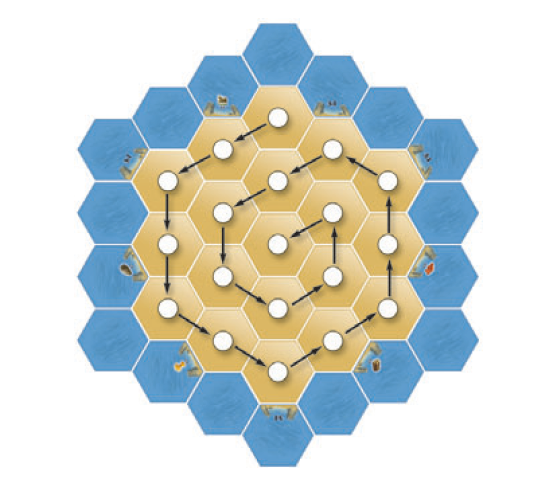
\includegraphics[width=6cm]{Bilder/Spielfeld-Blueprint.png}
	\caption{Verteilung der Zahlenchips auf dem Spielfeld (siehe Anhang Regelwerk S. 4)}
	\label{fig:Spielfeld-Blueprint}
\end{figure}

\textbf{Der Spielbeginn:}\\
Die ersten beiden Z�ge jedes Spielers laufen anders als die restlichen Z�ge des Spiels ab: In seinem ersten Zug darf jeder Spieler eine Siedlung und eine Stra�e platzieren ohne daf�r Ressourcen ausgeben zu m�ssen. Gleiches gilt f�r den zweiten Spielzug, wobei die Spieler ihre Geb�ude nun in entgegengesetzter Reihenfolge platzieren d�rfen. Nach dem zweiten Spielzug jedes Spielers erh�lt der jeweilige Spieler entsprechend Ressourcen f�r seine zweite Siedlung (jedes angrenzende Landschaftsfeld au�er der W�ste bringt ihm eine Ressource). In diesen ersten beiden Spielz�gen wird weder gew�rfelt, noch werden Ereigniskarten erworben.

\textbf{Gew�hnliche Spielz�ge:}\\
Die Reihenfolge, in der die Spieler ihre Z�ge machen, entspricht nun wieder der der ersten Spielrunde. Die gew�hnlichen Spielz�ge laufen von nun an  bis zum Ende des Spiels auf gleiche Weise ab: Zu Beginn seines Zuges w�rfelt der Spieler, woraufhin alle Spieler , wie bereits beschrieben, Ressourcen erhalten. Anschlie�end kann der Spieler, der jeweils am Zug ist, entweder etwas bauen oder eventuell handeln. Abschlie�end beendet der Spieler seinen Zug, sodass der N�chste dran ist. Im Detail l�uft ein gew�hnlicher Spielzug wie folgt ab:
\begin{enumerate}
	\item \textbf{W�rfeln:} Jeder Zug eines Spielers muss damit beginnen, dass er mit zwei W�rfeln w�rfelt. Anhand der Summe der Augen beider W�rfel, werden anschlie�end die Ressourcen verteilt. Wenn ein Zahlenchip der summierten Augenzahl entspricht, erh�lt ein Spieler mit einer Siedlung oder einer Stadt an diesem Feld f�r jede Siedlung die entsprechenden Ressourcen bzw. f�r jede Stadt jeweils zwei der entsprechenden Ressourcen.
	\item \textbf{Bauen:} Nachdem gew�rfelt wurde, kann gebaut werden. Zum Bau stehen  Stra�en, Siedlungen, St�dte und Entwicklungen (wenn diese Anforderung umgesetzt wird) zur Verf�gung, die mit den vorhandenen Ressourcen gekauft werden k�nnen.
	\item \textbf{(Handeln:)} Handeln kann entweder zum Abschluss des Spielzuges erfolgen oder bevor der Spieler baut. Da es sich hierbei jedoch um eine Kann-Anforderung handelt, wird dieser Spielbestandteil nur in Klammern angef�hrt. Ein Spieler kann entweder an den H�fen zu den jeweils angegebenen Verh�ltnissen,, mit der Bank im Verh�ltnis 4:1 oder mit einem anderen Spieler in einem beliebigen Verh�ltnis tauschen.
\end{enumerate}
\textbf{Ende des Spiels:}\\
Das Spiel endet, wenn einer der Spieler 10 Siegpunkte erreicht hat. Siegpunkte werden f�r unterschiedliche Errungenschaften im Spiel vergeben, so zum Beispiel f�r das Errichten von Siedlungen und St�dten, aber auch f�r die \textit{L�ngste Handelsstra�e} und die \textit{Gr��te Rittermacht}. F�r die Implementation kann die Vergabe der Siegpunkte danach angepasst werden, wie die Strategiefindung der KI-Spieler beeinflusst werden soll. Interessant w�re hierbei zu sehen, ob bei verschiedenen Siegbedingungen unterschiedliche KIs einen Vorteil haben. Es ist m�glich, dass eine KI, die das Bauen von Siedlungen favorisiert, mehr Spiele gewinnt, wenn dies mit mehr Siegpunkten belohnt wird. Stattdessen w�rde eine KI, die Wert auf l�ngere Handelsstra�en und mehr Ereigniskarten legt, bei einer diese Strategie beg�nstigenden Gewichtung vermehrt siegen.

\textbf{Baukosten:}\\
Es wurde bereits beschrieben, dass das Bauen Teil eines gew�hnlichen Spielzugs ist. Zum Bauen k�nnen alle f�nf verf�gbaren Ressourcen verwendet werden: Lehm, Holz, Schafe, Getreide und Stein. Die Kosten f�r die einzelnen Geb�ude setzen sich wie folgt zusammen:
\begin{enumerate}
	\item Stra�e: 1 Lehm, 1 Holz
	\item Siedlung: 1 Lehm, 1 Holz, 1 Schaf, 1 Getreide
	\item Stadt: 2 Getreide, 3 Stein
	\item Entwicklung: 1 Getreide, 1 Schaf, 1 Stein
\end{enumerate}

\textbf{Der R�uber:}\\
Die Implementation des R�ubers ist Teil der Kann-Anforderungen. Sollte er jedoch implementiert werden, so sind zwei Varianten vorstellbar: Entweder wird der R�uber wird im vollen Umfang, was bedeutet, dass ein Spieler, der eine Sieben w�rfelt, den R�uber auf ein Feld setzen darf, welches dadurch keine Ressourcen mehr liefert. Au�erdem k�nnte der jeweilige Spieler in dieser Variante einen gegnerischen Spieler ausw�hlen, der eine Siedlung oder eine Stadt an diesem Landschaftsfeld hat und ihm eine zuf�llig ausgew�hlte Ressource stehlen. Alternativ hierzu kann nur der erste Teil umgesetzt werden, indem der R�uber zwar Felder blockiert, aber keinen Diebstahl erm�glicht.

\textbf{H�fen:}\\
In der Sektion \textit{Gew�hnliche Spielz�ge} wird bereits das Handeln an H�fen erw�hnt. H�fen sind Teil der Kann-Anforderungen und somit nicht zwingend Teil des Spiels. Sollten sie jedoch implementiert werden, sind verschiedene Stufen der Implementation denkbar: Die Mindestanforderung w�re, dass ein Spieler nur an einem Hafen handeln kann, wenn dieser eine Siedlung oder eine Stadt im Einzugsbereich dieses Hafens besitzt. \\
Im Brettspiel gibt es mehrere Arten von H�fen. Einige dieser H�fen sind an Rohstoffe gebunden und k�nnen im Verh�ltnis 2:1 f�r den Handel genutzt werden. Das bedeutet, beim Handel an einem Holzhafen w�rde eine Einheit Holz zwei Einheiten eines anderen Ressource kosten. Neben diesen gebundenen H�fen existieren auch ungebundene. Diese bieten ein Verh�ltnis von 3:1, sodass drei Einheiten eines Rohstoffes f�r eine Einheit eines beliebigen anderen Rohstoffes eingetauscht werden k�nnen. Als Abstufungen f�r die Implementation ist es denkbar, zun�chst nur die ungebundenen und anschlie�end auch die gebundenen H�fen umzusetzen. \\
Betrachtet man den Handel an H�fen im gesamten Kontext des Spiels, l�sst sich feststellen, dass die Kann-Anforderung \textit{Handel} zumindest als sp�tere Weiterentwicklung der Software zu empfehlen ist. Hierbei ist wahrscheinlich der Handel mit der Bank am wichtigsten, gefolgt vom Handel an den H�fen und dem Handel zwischen den Spielern. Eventuell k�nnte der Handel zwischen den Spielern auch h�her als der Bank- und Hafenhandel priorisiert werden, da dieser einen interessanten strategischen Aspekt darstellt. \\
Er erscheint jedoch sinnvoll, den Bankhandel als erste Erweiterung der der Software zu Verf�gung zu stellen, da es ohne diesen  zu Konstellationen kommen kann, in denen ein oder mehrere Spieler im Spiel nicht mehr vorankommen k�nnen. Dieser Zustand kann entstehen, wenn die Anfangssiedlungen ungeschickt platziert werden und kein Zugang zu den - f�r Stra�en und Siedlungen n�tigen - Rohstoffen besteht. F�r einen Spieler, der sich in einer solchen Situation befindet, ist Handel der einzige Ausweg, da es ansonsten keine realistische Chance f�r ihn gibt, das Spiel noch f�r sich zu entscheiden. Eine genauere Erl�uterung dieser Erweiterung ist in Kapitel \ref{sec:Ausblick} zu finden.

\section{Konzeption der Schnittstelle}
In diesem Kapitel wurden zwar bereits Aussagen �ber die Schnittstelle getroffen und Anforderungen an diese gestellt, jedoch wurde noch nicht erl�utert, wie diese realisiert werden kann. Entsprechend soll letzteres hier nachgeholt werden, wobei zu beachten ist, dass die Umsetzung der Schnittstelle zur Erf�llung der Anforderungen in einer bestimmten Weise erfolgen muss: Betrachtet man nochmals die gestellten Anforderungen, so lassen sich die ersten beiden bereits dadurch l�sen, dass JSON als Kommunikationsmedium genutzt wird. Anforderung 3 (s.o.) h�ngt eng mit einer korrekten Umsetzung zusammen, was zwar wichtig ist, jedoch das Konzept an sich nicht beeinflusst. Aus Anforderung 4 (s.o.) hingegen lassen sich deutlich mehr Aspekte extrahieren. Diese besagt, dass eine KI einem realen Spieler gegen�ber keine Vor- oder Nachteile haben darf, die allein dadurch entstehen, dass sie eine KI ist. Dieser Zusammenhang kann auch als Fairness aufgefasst werden. Konkret bedeutet das f�r die Umsetzung, dass eine KI nur die gleichen Optionen zu den jeweiligen Zeitpunkten im Spiel wie ein menschlicher Spieler hat. Hieraus geht hervor, dass das Timing einer Rolle f�r die Anfragen und deren Verarbeitung spielt. Wenn eine KI beispielsweise den Bau einer Siedlung anfragt w�hrend sie nicht an der Reihe ist, muss der Bau einer solchen Siedlung abgelehnt werden. Da das Spiel zu jeder Zeit wei�, wer an der Reihe ist, kann festgelegt werden, dass nur die Anfragen des Spielers verarbeitet werden, der auch gerade einen Spielzug ausf�hrt. Das Zustand eines Zuges selbst, ist jedoch auch von Relevanz, da ein Spielzug immer mit dem Rollen der W�rfel beginnen muss. Am besten lie�e sich dieses Problem dadurch l�sen, Anfragen nur in einer bestimmten Reihenfolge zu erlauben: Zun�chst w�rde gew�rfelt und erst anschlie�end daran k�nnte gehandelt oder gebaut werden, ein  erneutes W�rfeln w�rde dabei verhindert. Beendet die KI  ihren Spielzug, verl�re sie die Berechtigung dazu, Anweisungen jeglicher Art ausf�hren zu lassen, wieder. Zudem sind in den ersten beiden Z�gen jedes Spielers Aktionen erlaubt, die in den restlichen Aktionen nicht zugelassen werden w�rden (siehe Kapitel \ref{sec:regeln}), was auch einen Einfluss auf das Annehmen einiger Anfragen hat. Optimal lie�e sich dieses Problem l�sen, indem im Spiel selbst eine Verzahnung der KIs und der menschlichen Spieler erfolge. Damit ist gemeint, dass die gleichen Bedingungen f�r KIs genutzt werden, die auch einem realen Spieler Funktionen freischalten oder sperren.

Ein weiterer wichtiger Aspekt, der durch die Anforderungen aufgegriffen wird, ist der Umgang mit Informationen. Anforderung 4 (s.o.) beschreibt zus�tzlich, dass eine KI zu keinem Zeitpunkt im Spiel prinzipiell bevorteilt oder benachteiligt werden darf. Wichtig ist hierbei, dass die Schnittstelle nicht dauerhaft alle Informationen senden muss, sondern dass das grundlegende Vorhandensein der M�glichkeit ausreicht. Wahrscheinlich werden die initialen KIs nicht alle Informationen ben�tigen bzw. verarbeiten k�nnen, die ein Mensch nutzen w�rde. Allerdings sollte das Format grundlegend auch umfangreichere Informationen �bermitteln k�nnen. Dieses Prinzip ist analog zur Interaktion mit einem realen Spieler. Das Spiel h�lt die Informationen auf der Spielfl�che aktuell, zwingt den Spieler jedoch nicht, diese auch zu jedem Zeitpunkt wahrzunehmen. Er schaut sie sich bei Bedarf an. Genauso sollte auch mit einem KI-Spieler verfahren werden. Wenn die KI Informationen anfragt, auf die auch ein realer Spieler Zugriff hat, werden diese �bermittelt, aber sie werden nicht dauerhaft gesendet. Diese �berlegung k�nnte dazu f�hren, dass der Zeitpunkt des Anfragens zu einem strategischen Element wird -  allerdings nur dann,  wenn die Anzahl der Anfragen begrenzt wird, was hier nicht der Fall ist, da ein realer Spieler auch in der Lage ist, Informationen beliebig oft wahrzunehmen.

Anforderung 5 (s.o.) geht in die gleiche Richtung wie die eben beschriebene, wobei hier der Fokus auf dem Sch�tzen der versendeten Informationen liegt. �hnlich zum realen Spieler, der seine Ressourcen vor den Gegnern geheim halten kann, muss es auch einer KI erm�glicht werden, die Menge an Ressourcen und den Inhalt seiner Anfragen vor den Gegnern zu verschleiern. Lediglich das, was auf dem Spielfeld vonstatten geht, sollte den Gegnern einen Einblick in die Strategie eines Spielers erm�glichen. Daher ist es wichtig, die Antwort des Spiels als Einzelnachricht zu realisieren und nicht allen in Form eines Broadcasts mitzuteilen. Es klingt m�glicherweise trivial, soll hier aber erw�hnt werden, weil es einen fundamentalen Beitrag zur Fairness liefert. \\
Aus den Ausf�hrungen Anforderung 4 und 5 (s.o.) geht zudem die Einhaltung der Anforderung 6 (s.o), realen und KI-Spielern grundlegend die gleichen Informationen bereitstellen zu k�nnen wie realen Spielern, hervor.

Durch die Einhaltung der beschriebenen Anforderungen seitens des Spiels wird den KIs eine hohe Gestaltungsfreiheit gelassen. Dadurch, dass die KIs entscheiden k�nnen, wann sie Informationen �ber Ressourcen abfragen, m�ssen sie ihre Strategie nicht an den Zeitpunkt des Erhaltens der Information anpassen. Dennoch gibt es einige Anweisungen, die das Spiel an die KI-Spieler senden muss, ohne auf Anfragen von diesen zu warten: Das betrifft zum Beispiel die Information dar�ber, ob ein Spieler gerade an der Reihe ist. Hier w�rde eine Abfrage durch jeden Spieler keinen Sinn ergeben, weil diese dauerhaft erfolgen m�ssten. Einfacher ist es f�r den Ablauf des Spiels, wenn das Spiel nach jedem Spielerwechsel eine Nachricht an die Spieler sendet. Ferner m�ssen pl�tzliche Ereignisse sofort an die Spieler �bermittelt werden. Das beste Beispiel hierf�r ist das Nutzen des R�ubers. Wenn der R�uber versetzt wird und einem Spieler eine Ressourcenkarte entwendet wird, muss dies ? zumindest den betroffenen Spielern - unmittelbar mitgeteilt werden, da dies m�glicherweise wichtig f�r die Strategiebildung ist. Allgemein k�nnte auch eine Art doppelte Absicherung eingef�hrt werden, bei denen �nderungen an den Best�nden von Ressourcen eines Spielers direkt �bermittelt werden, aber zus�tzlich Abfragen durch die KI erfolgen k�nnen, um es dieser zu erm�glichen, vor dem Bau von Siedlungen, Stra�en, etc. auf jeden Fall Informationen �ber die aktuelle Zahl an verf�gbaren Ressourcen zu haben.

Neben den hier offensichtlichen Anfragen und Antworten gibt es weitere fundamentale Informationen, �ber die jede KI verf�gen muss. Die fundamentalste ist hierbei die �ber den Aufbau des Spielfelds: Jede KI muss wissen, welches Feld an welcher Stelle liegt, damit sie eine Strategie bilden kann. Da die Initialisierung des Spielfelds jedoch nur zu Beginn erfolgt und das Spielfeld danach gleichbleibend ist, sollte eine Art Initialisierungsnachricht an die KI-Spieler gesendet werden, sobald das Spiel fertig initialisiert ist, um das Entwickeln einer anf�nglichen Strategie zu erm�glichen. Zur Veranschaulichung folgt eine Tabelle aller Anfragen und Antworten, inklusive der jeweiligen Zeitpunkte, Absender und Empf�nger. Die gezeigten Nachrichten verdeutlichen, wie umfangreich die Kommunikation zwischen Spiel, Schnittstelle und dem computergesteuerten Spieler werden kann. Es wird jede T�tigkeit abgebildet, die auch einem menschlichen Spieler zur Verf�gung stehen w�rde. Dies w�rde der Implementierung aller Anforderungen gleichkommen.


\begin{table}
	\caption{Geplante Kommunikation zwischen Schnittstelle und KI-Spieler}
	\label{tab:Nachrichten}
	\begin{tabularx}{15cm}{X|X|X|X|X}
		\fett{Nachricht} & Absender & Empf�nger & Zeitpunkt & Aktion/Antwort\\
		\hline
		Aufbau Spielfeld & Spiel & Spieler & Nach Initialisierung & Empfangs-
		best�tigung \\
		\hline
		Siedlungsbau- men� �ffnen/ schlie�en & Spieler & Spiel & Im eigenen Zug nach W�rfeln & Men� �ffnen, schlie�en oder ablehnen \\
		\hline
		Bau Siedlung & Spieler & Spiel & Im eigenen Zug bei ge�ffneten Baumen� & Bau Siedlung oder ablehnen \\
		\hline
		Stadtbaumen� �ffnen/ schlie�en & Spieler & Spiel & Im eigenen Zug nach W�rfeln & Men� �ffnen, schlie�en oder ablehnen \\
		\hline
		Bau Stadt & Spieler & Spiel & Im eigenen Zug bei ge�ffneten Baumen� & Bau oder ablehnen \\
		\hline
		Stra�enbaumen� �ffnen/ schlie�en & Spieler & Spiel & Im eigenen Zug nach W�rfeln & Men� �ffnen, schlie�en oder ablehnen \\
		\hline
		Bau Stra�e & Spieler & Spiel & Im eigenen Zug bei ge�ffneten Baumen� Bau oder ablehnen & Bau Stra�e oder ablehnen \\
		\hline
		Kauf Ereigniskarte & Spieler & Spiel & Im eigenen Zug nach W�rfeln & Ereigniskarte \\
		\hline
		Einsatz Ereigniskarte & Spieler & Spiel & Im eigenen Zug nach W�rfeln & Effekt \\
		\hline
		Verschiebung R�uber & Spiel & Spieler & Bei gew�rfelter Sieben oder Ereigniskarte & Spiel �ffnet Verschiebunsmen� f�r Spieler\\
		\hline
	\end{tabularx}
\end{table}

\begin{table}
	\caption{Geplante Kommunikation zwischen Schnittstelle und KI-Spieler (Fortf�hrung)}
	\label{tab:Nachrichten2}
	\begin{tabularx}{15cm}{X|X|X|X|X}
		Diebstahl Ressource & Spiel & Spieler & Nach Verschiebung des R�ubers & Spiel �ffnet Diebstahlmen� \\
		\hline
		Spielende & Spiel & Spieler & Wenn ein Spieler die Mindestanzahl der n�tigen Siegespunkte erreicht & Spiel verk�ndet Sieger als Broadcast \\
		\hline
		Aktualisierung Ressourcen & Spiel & Spieler & nach jeder �nderung der Ressourcen eines Spielers & Spiel versendet die neuen Mengen der Ressourcen. \\
		\hline
		Zugende & Spiel & Spieler & Zum Ende eines Zuges nach dem W�rfeln & Broadcast: Aktualisierung aktueller Spieler \\
		\hline
		W�rfeln & Spieler & Spiel & Zu Beginn jedes Zuges & Summe der Augen \\
		\hline
		Ressourcen- abfrage & Spieler & Spiel & Bei Bedarf & Spiel antwortet mit Aktualisierung Ressourcen \\
		\hline
		Handelsanfrage & Spieler & Spieler & Im Spielzug nach dem W�rfeln & Schnittstelle erm�glicht eine Antwort durch andere Spieler ja/nein \\
		\hline
	\end{tabularx}
\end{table}


\chapter{Implementation}
\definecolor{bluekeywords}{rgb}{0,0,1}
\definecolor{greencomments}{rgb}{0,0.5,0}
\definecolor{redstrings}{rgb}{0.64,0.08,0.08}
\definecolor{xmlcomments}{rgb}{0.5,0.5,0.5}
\definecolor{types}{rgb}{0.17,0.57,0.68}


\lstset{language=[Sharp]C,
	captionpos=b,
	%numbers=left, %Nummerierung
	%numberstyle=\tiny, % kleine Zeilennummern
	frame=lines, % Oberhalb und unterhalb des Listings ist eine Linie
	showspaces=false,
	showtabs=false,
	breaklines=true,
	showstringspaces=false,
	breakatwhitespace=true,
	escapeinside={(*@}{@*)},
	commentstyle=\color{greencomments},
	morekeywords={partial, var, value, get, set},
	keywordstyle=\color{bluekeywords},
	stringstyle=\color{redstrings},
	basicstyle=\ttfamily\small,
}

Dieses Kapitel soll sich mit der Umsetzung der im Entwurf beschriebenen Software befassen. Es werden das Spiel, die Schnittstelle und die initialen KI-Spieler erl�utert, wobei chronologisch vorgegangen wird, sodass  zun�chst eine grundlegende Version des Spiels beschrieben und anschlie�end auf die Umsetzung der Schnittstelle eingegangen wird. Anschlie�end wird die Weiterentwicklung des Spiels und seiner anderen Bestandteile fokussiert. Die Implementation der initialen KIs wird zuletzt betrachtet. \\
Nach der Erl�uterung der Implementation werden Anpassungen beschrieben, die zuvor zwar nicht so geplant wurden,  w�hrend der Umsetzung jedoch trotzdem Einzug ins Programm erhielten bzw. ausgelassen wurden.

\section{Verwendete Technologien}
\label{sec:Technologien}
Zu Beginn des Kapitels \ref{cha:Entwurf} wird bereits thematisiert, dass f�r die Erstellung der Software \textit{Unity}, \textit{C\#} und \textit{JSON} f�r die Schnittstelle verwendet werden sollen. In diesem Abschnitt soll noch einmal genauer auf die verwendeten Technologien eingegangen und die Entscheidung f�r diese Technologien begr�ndet werden.

\textit{Unity} ist eine Spieleentwicklungsengine, die eine schnelle und einfache Entwicklung komplexer Spieler erm�glicht. Zur Wahl standen entweder die \textit{Unity}-Engine oder die \textit{Unreal}-Engine. Obwohl f�r dieses Projekt beide Optionen infrage gekommen w�ren, fiel die Entscheidung auf \textit{Unity}, welches  sich vor allem durch den sehr umfangreichen \textit{Asset-Store} und somit durch die M�glichkeit, einfacher Importe vielerlei kostenloser Grafiken, Animationen und Sounds sowie  die Entwicklung beschleunigenden Funktionalit�ten, aus. Au�erdem ist \textit{Unity} subjektiv gesehen benutzerfreundlicher als die \textit{Unreal}-Engine.\\
Auch \textit{Unreal} bietet einige Vorteile gegen�ber \textit{Unity}, die jedoch f�r diese Arbeit keinen nennenswerten Mehrwert bieten,  weshalb die Entscheidung im Hinblick auf die Ziele dieser Arbeit auf die Verwendung von \textit{Unity} fiel, zumal der Fokus haupts�chlich auf der Logik des Spiels liegt und nicht auf den grafischen Feinheiten.

Mit der Verwendung von \textit{Unity} wurden auch die m�glichen Programmiersprachen stark eingeschr�nkt. Bis zur Version 2017.1 war es m�glich neben \textit{C\#} auch in JavaScript und \textit{Boo} zu programmieren, seit der Ver�ffentlichung dieser Version ist \textit{C\#} jedoch die einzig verwendbare Programmiersprache. Entsprechend fiel die Wahl der Programmiersprache f�r dieses Projekt auf \textit{C\#}.  \\
\textit{C\#} ist eine plattformunabh�ngige, objektorientierte Programmiersprache, die starke �hnlichkeiten zu \textit{Java} und \textit{C++} aufweist. Neben dem objektorientierten Paradigma ist jedoch auch funktionale oder imperative Programmierung m�glich.

Die Schnittstelle soll durch \textit{JSON} (\textit{JavaScript Object Notation}) realisiert werden, womit gemeint ist, dass \textit{JSON} das gew�hlte Format der Informations�bertragung zwischen Spiel und KI-Spieler ist. \textit{JSON} soll durch das folgende Beispiel veranschaulicht werden:\\

\textbf{KI-Anfrage:} \\
\{\\
\null\quad \quotes{spieler}: \quotes{1} \\
\null\quad \quotes{aktion}: \quotes{Wuerfeln}\\
\}
\\
\\
\textbf{Spiel-Antwort:} \\
\{\\
\null\quad \quotes{augenzahl}: 8 \\
\null\quad \quotes{ressourcen}: [ \\
\null\quad\quad \{ \\
\null\quad\quad\quad \quotes{name}: \quotes{lehm} \\
\null\quad\quad\quad \quotes{anzahl}: 2 \\
\null\quad\quad\}, \\
\null\quad\quad \{ \\
\null\quad\quad\quad \quotes{name}: \quotes{holz} \\
\null\quad\quad\quad \quotes{anzahl}: 1 \\
\null\quad\quad\}, \\
\null\quad]\\
\}

Das Beispiel zeigt mehrere Aspekte des \textit{JSON}-Formats: zu sehen sind zwei Dateien, einerseits die gesendete Anfrage durch die KI und andererseits die Antwort des Spiels.

Aus dem Beispiel geht hervor, dass innerhalb der geschweiften Klammern Variablen definiert werden, die einen Wert enthalten. Auff�llig ist insbesondere, dass nicht typisiert wird, sondern ohne Auskunft �ber den Variablentyp verschickt wird.

Eine Zeile, die ein Attribut beschreibt, besteht aus dem Namen der Variable in Anf�hrungszeichen, gefolgt von einem Doppelpunkt und dem zugewiesenen Wert. Zeichenketten wie der Name eines Attributes werden in Anf�hrungszeichen gesetzt, wohingegen Zahlen ohne dastehen. Deutlich wird dies bei den Attributen \textit{spieler} (KI-Anfrage) und \textit{augenzahl} (Spiel-Antwort). Im ersten Fall handelt es sich um einen Namen, im zweiten um eine Anzahl. 

Des Weiteren lassen sich Listen per \textit{JSON}-Format verschicken. So enth�lt die zweite Datei eine Liste der Ressourcen eines Spielers und schickt ihm diese als Teil der Antwort zu. Es werden nachfolgend aus Platzgr�nden nur zwei Ressourcen beispielhaft angegeben. Listen werden mit eckigen Klammern ge�ffnet und geschlossen. Innerhalb einer solchen Sektion werden einzelne Objekte durch Kommata getrennt und von geschweiften Klammern umschlossen definiert.

Ob in diesem Fall die Verwendung einer Liste n�tig wird, ist fraglich, doch dieses Beispiel dient, wie erw�hnt, lediglich der Veranschaulichung und muss daher nicht zwingend in gleicher Weise sp�ter implementiert werden. Weiterhin ist zu diskutieren, ob das Spiel �berhaupt mit den Ressourcen eines Spielers auf das W�rfeln antworten muss oder ob hierf�r eine weitere Anfrage erfolgen sollte. 

\section{Die grundlegende Umsetzung des Spiels}
\label{sec:Spiel}
In Abschnitt \ref{sec:Technologien} wurde auf die Gr�nde der Verwendung von \textit{Unity} f�r die Umsetzung des Spiels eingegangen. Einer ist, dass mit verh�ltnism��ig geringem Aufwand eine ansprechende Nutzeroberfl�che gestaltet werden kann. Die Grafiken und die Formen der Objekte, die im Spiel verwendet werden, stammen aus einer anderen Implementation von \textit{Siedler von Catan}, die auf Github unter \textit{https://github.com/buttsj/unity-settlers-of-catan} zu finden ist (\cite{Butt2016}).

\begin{figure}[h]
	\centering
	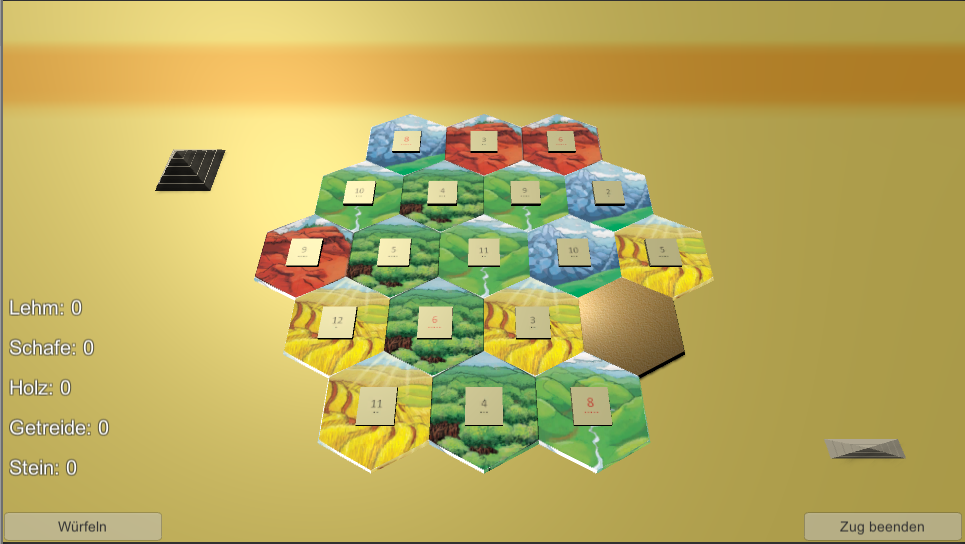
\includegraphics[width=16cm]{Bilder/SpielfeldStartoberflaeche.png}
	\caption{Nutzeroberfl�che zu Beginn des Spiels (\cite[vgl.]{Butt2016})}
	\label{fig:Nutzeroberfl�che}
\end{figure}

Abbildung \ref{fig:Nutzeroberfl�che} zeigt eine so gestaltete Oberfl�che. Hierbei fallen mehrere Aspekte ins Auge. Zun�chst einmal das Spielfeld selbst. Dieses besteht wie das Original aus insgesamt 19 sechseckigen Einzelteilen. Die Verteilung der Sechsecke erfolgt nach folgender Verf�gbarkeit: viermal Wald, viermal Getreide, dreimal Ziegel, dreimal Stein, dreimal Schaf, einmal W�ste. Auff�llig ist, dass das W�stenfeld als einziges ohne Nummer bleibt, was daran liegt, dass es keine Ressourcen liefert, wenn ein Spieler eine Siedlung an diesem Feld gr�ndet. \\
Links ist eine Art Pyramide, die eine Siedlung darstellen soll, zu sehen. Dementsprechend befindet sich im unteren rechten Bereich des Bildes das Abbild einer Stra�e. Neben den Objekten in der Umgebung sind im Sichtfeld des Nutzers ebenso zwei ausgegraute Buttons (W�rfeln und Zug beenden) und eine Anzeige, die die verf�gbaren Ressourcen des aktuellen Spielers darstellt, zu sehen. \\

\subsection{Die Generierung des Spielfelds}

\lstinputlisting[label=lst:MapGenerator1,caption={Spielfeld-Generator Startmethode}]{Listings/MapGenerator1.cs}

Listing \ref{lst:MapGenerator1} und \ref{lst:MapGenerator2} zeigen wie die Erstellung des beschriebenen Spielfelds zustande kommt. In der gezeigten Startmethode werden mehrere Listen deklariert und initialisiert. Die Liste \textit{resources} enth�lt Materialien - jeweils in der Anzahl, in der sie sp�ter auf dem Spielfeld vorkommen d�rfen. Neben dieser Liste existieren weitere. Eine speichert beispielsweise alle Sechsecke, sodass diese sp�ter angesteuert werden k�nnen. Eine andere speichert die Materialien der Nummern auf den Sechsecken. Zudem stehen zwei Listen zur Verf�gung, die Ganzzahlen speichern. Zum Ende der Startmethode wird die Liste \textit{tiles} ohne Inhalt initialisiert, bevor \textit{CreateMap(List<Material> resources, List<Material> numbers, List<GameObject> tiles, List<int> positions, List<GameObject> hexTiles, List<int> ints)} aufgerufen wird. \\

\lstinputlisting[label=lst:MapGenerator2,caption={Spielfeld-Generator CreateMap-Methode}]{Listings/MapGenerator2.cs}

Listing \ref{lst:MapGenerator2} zeigt wie die Oberfl�che f�r jedes neue Spiel generiert wird. Zu Beginn wird eine foreach-Schleife ge�ffnet, die einmal f�r jedes in hexTiles enthaltene Sechseck (GameObject) durchlaufen wird. Innerhalb dieser Schleife wird zun�chst die Oberfl�che des aktuellen Sechsecks als Variable sowie die Nummer auf dem Sechseck zwischengespeichert. Daraufhin wird zuf�llig eine Zahl generiert, die zwischen 0 (inklusive) und der Gr��e der Menge an verf�gbaren Landschaften liegt (exklusive). Nun kann im n�chsten Schritt das Material an der Stelle dieser zuf�lligen Zahl der Liste \textit{resources} dem aktuellen Sechseck als Oberfl�che zugeordnet werden, wie in Zeile zw�lf zu sehen ist. Anschlie�end wird, um eine Doppelvergabe zu vermeiden, das vergebene Material aus der \textit{resources} Liste entfernt. \\
In den darauffolgenden Zeilen, wird daf�r gesorgt, dass nur Sechsecke, die ein anderes Landschaftsfeld als die W�ste repr�sentieren, eine Zahl erhalten. Au�erdem werden die Zahlen entsprechend einer bestimmten Reihenfolge vergeben. Diese Reihenfolge ist durch die Listen \textit{numbers} und \textit{ints} vorgegeben. \textit{numbers} enth�lt die passenden Materialien und \textit{ints} eine Repr�sentation dieser Materialien als Ganzzahlen, um anderen Skripten sp�ter einen einfachen Zugriff zu erm�glichen. \\
Wenn eine Zahl einem Sechseck zugewiesen wurde, dann wird diese aus dem beiden Listen entfernt. Sollte es sich bei dem betrachteten Sechseck um die W�ste gehandelt haben, so wird das Pl�ttchen auf diesem Feld gel�scht, damit es nicht ohne Zahl auf dem Feld zur�ckbleibt und die Sichtbarkeit der W�ste verringert wird.

%\lstinputlisting[label=lst:Tile,caption={Hilfsklasse Tile}]{Listings/Tile.cs}
Diese Zuweisung der Zahlen als Integerwerte, kann nur deshalb erfolgen, weil es eine Hilfsklasse \textit{Tile} gibt, die Teil des Prefabs der Sechsecke ist und �ber ein Attribut verf�gt, welches die Nummer speichert. Jedoch verf�gt \textit{Tile} neben der Speicherung eines Integerwertes �ber keinerlei Funktionalit�t und ist daher nur als Hilfsklasse zu bezeichnen, weshalb sie nur im Anhang abgebildet ist.. 

Insgesamt garantiert die gew�hlte Umsetzung eine Variabilit�t im Aufbau des Spielfelds: Bei jedem Spielstart werden die Felder in eine andere Reihenfolge gebracht, sodass die gleiche Positionierung der Siedlungen in allen Spielen f�r die Spieler zu teilweise unterschiedlichen Ergebnissen f�hrt. Dennoch bietet die Abspeicherung der Zahlen auf den Feldern und die Sicherung des Zugriffs auf die Oberfl�che jedes Sechsecks die M�glichkeit, dass weitere Skripte die Informationen verwenden, ohne einen Umweg zu gehen.

\subsection{Der Spieler}
\label{sub:Player}
Um das Spiel spielen zu k�nnen, muss es eine Repr�sentation des computergesteuerten oder menschlichen Spielers geben, der dessen Anweisungen ausf�hrt. Hierzu wurde ein Skript \textit{PlayerScript} erstellt. Im Spiel selbst besitzt ein leeres \textit{GameObject} dieses Skript und wird damit zu einem Spieler. Hierdurch k�nnen theoretisch beliebig viele Spieler eingef�gt werden.\\

\lstinputlisting[label=lst:PlayerScript1,caption={Attribute des Spielers}]{Listings/PlayerScript1.cs}

In Listing \ref{lst:PlayerScript1} ist der Beginn des \textit{PlayerScripts} zu sehen. Es verf�gt �ber eine Vielzahl an Attributen, die unterschiedlichen Funktionen dienen. So braucht es einen eigenen Vector3, der die Perspektive, aus der der Spieler auf das Spielbrett schaut, beschreibt und auf die die ebenfalls als Attribut gespeicherte \textit{Camera} angewendet werden kann. Des Weiteren verf�gt der Spieler �ber die Vorlage (den Prefab) zum Bau von Siedlungen (GameObject village) und Stra�en (GameObject road), sowie �ber eine Farbe, in der sp�ter seine Objekte auf dem Spielfeld erscheinen. 

Zudem m�ssen seine verf�gbaren Ressourcen gespeichert und eine M�glichkeit der Ausgabe durch Textfelder gegeben werden. Zus�tzlich stellen die Variablen \textit{isFirstTurn} und \textit{isSecondTurn} eine M�glichkeit dar, zu pr�fen, ob der Spieler sich in einem der ersten beiden Z�ge befindet - eine Zeit, in der Spieler kostenlos bauen darf. Dieses kostenlose Bauen kann dann durch \textit{bool freeBuild} bzw. \textit{bool freeBuildRoad} ermittelt werden. Schlie�lich braucht es neben zwei Listen, die alle Siedlungen (List<GameObject> villages) und alle Stra�en (List<GameObject> roads) sowie die Anzahl an Siegpunkten und die L�nge der l�ngsten Stra�e des Spielers speichern. \\

\lstinputlisting[label=lst:PlayerScript1StartAwake,caption={Initialisierung des Spielers}]{Listings/PlayerScript1StartAwake.cs}

Die in Listing \ref{lst:PlayerScript1StartAwake} abgebildete Methode \textit{private void Awake()} initialisiert einige der Attribute auf ihre Anfangswerte, die Methode \textit{void Start()} (ebenfalls in Listing \ref{lst:PlayerScript1StartAwake} abgebildet) erreicht im Grunde das Gleiche, wird aber nach der Awake-Methode aufgerufen. Dies ist an dieser Stelle notwendig, um sichergehen zu k�nnen, dass die Text-Objekte bereits erzeugt wurden, wenn auf diese zugegriffen wird. Au�erdem werden die Liste der Siedlungen und die der Stra�en jeweils als leere Listen initialisiert.

\lstinputlisting[label=lst:PlayerScript2,caption={Attribute und Initialisierung des Spielers}]{Listings/PlayerScript2.cs}

In Listing \ref{lst:PlayerScript2} sind die Methoden gezeigt, die zu Beginn eines Zuges aufgerufen werden m�ssen. FirstTurn() wird nur im ersten Zug aufgerufen, \textit{SecondTurn()} nur im zweiten und Turn() zu Beginn jedes anderen Zuges. Alle drei Methoden beginnen damit, dass sie die Methode \textit{AdjustCamera()} aufrufen. Hierbei handelt es sich um eine Methode, die die Position der gespeicherten Kamera auf die Perspektive des Spielers setzt. Anschlie�end werden die bool-Werte zur Identifikation des Zuges entsprechend gesetzt sowie festgelegt, ob in diesem Zug kostenlos gebaut werden darf. In den Methoden f�r die ersten beiden Z�ge wird daher \textit{freeBuild} auf \textit{true} gesetzt, \textit{freeBuildRoad} jedoch auf \textit{false}. \textit{freeBuildRoad} wird erst \textit{true}, sobald die kostenlose Siedlung des aktuellen Zuges gebaut wurde. In \textit{Turn()} darf nicht kostenlos gebaut werden, weshalb \textit{freeBuild} und \textit{freeBuildRoad} auf \textit{false} gesetzt werden und bis zum Ende des Spiels auf diesem Wert bleiben.

\lstinputlisting[label=lst:PlayerScript3,caption={Attribute und Initialiserung des Spielers}]{Listings/PlayerScript3.cs}

Nachdem Listing \ref{lst:PlayerScript2} und Listing \ref{lst:PlayerScript1} die Initialisierung des Spielers und seiner Z�ge zeigten, bringt Listing \ref{lst:PlayerScript3} die erste Funktionalit�t mit sich: Abgebildet sind zwei Methoden. Erstere (\textit{HasRessoucesForVillage()}) �berpr�ft , ob der Spieler genug Ressourcen zum Bau einer Siedlung hat, die zweite Methode (\textit{HasRessourcesForRoad()}) bewerkstelligt dies analog f�r die Stra�en. F�r eine Siedlung ben�tigt der Spieler jeweils eine Einheit Lehm, Holz, Schafe und Getreide. F�r eine Stra�e nur jeweils eine Einheit Holz und Lehm. �ber die Ressourcenvariablen wird abgefragt, ob diese Rohstoffe vorhanden sind. Dementsprechend wird ein bool-Wert zur�ckgegeben.

\lstinputlisting[label=lst:PlayerScript4,caption={Attribute und Initialiserung des Spielers}]{Listings/PlayerScript4.cs}

Neben dem Bau von neuen Siedlungen, muss auch der Nutzen einer solchen ermittelt werden. Jede Siedlung kann dem Besitzer bestimmte Rohstoffe einbringen. Hierzu existieren zwei Methoden \textit{CollectResourcesForVillage(GameObject village)} und \textit{CollectResources(int number)}. Beide erreichen im Grunde das Gleiche, wobei \textit{CollectResourcesForVillage(GameObject village)} die Rohstoffe f�r eine konkrete Siedlung sammelt und \textit{CollectResources(int number)} abh�ngig von der gew�rfelten Nummer die Rohstoffe verteilt. Exemplarisch ist in Listing \ref{lst:PlayerScript4} nur \textit{CollectResources(int number)} aufgef�hrt. Die andere ist �quivalent und daher nur im Anhang zu finden. \\
Zu jeder Siedlung werden die angrenzenden Felder gespeichert. Diese k�nnen entweder \textit{null} oder von einem bestimmten Typus sein, der �ber dessen \textit{Material} abgefragt wird. Auf diese Weise kann durch verschachtelte if-Verzweigungen ermittelt werden, ob und welche Rohstoffe dem Spieler zuzusprechen sind. Am Ende beider Methoden wird \textit{UpdateResources()} aufgerufen, eine Methode, die die aktualisierten Mengen an Rohstoffen ausgibt. 

\lstinputlisting[label=lst:PlayerScript5,caption={Attribute und Initialisierung des Spielers}]{Listings/PlayerScript5.cs}

Nachdem oben erl�utert wurde, wie die Ermittlung der n�tigen Menge an Rohstoffen zum Bau einer Siedlung oder Stra�e erfolgt und der Ertrag einer Siedlung berechnet wird, stellt Listing \ref{lst:PlayerScript5} den tats�chlichen Bau von Siedlungen und Stra�en dar. Die Methode \textit{BuildVillage(Vector3 position)} bekommt als Parameter die Position f�r den Bau der Siedlung �bergeben und kann diese dort platzieren. Zu Beginn der Methode wird �berpr�ft, ob der Spieler kostenlos bauen darf bzw. ob er genug Rohstoffe zum Bauen hat. Falls er genug Rohstoffe hat, aber nicht kostenlos bauen darf, bezahlt der Spieler entsprechend mit den Rohstoffen. Wenn allerdings kostenlos gebaut werden darf, wird die M�glichkeit des kostenlosen Bauens genutzt. Anschlie�end w�rde dann der kostenlose Bau einer Stra�e erlaubt werden.

In jedem Fall wird im Anschluss an diese Pr�fung eine neue Siedlung auf Grundlage des \textit{GameObjects village} instanziiert. Bei dem instanziierten Objekt handelt es sich um eine weitere Instanz, des bereits als Repr�sentation instanziierten und daf�r vorgesehenen \textit{Prefabs}. Dieser Instanz wird die zuvor �bergebene Position zugeschrieben und sie erh�lt die Farbe des Spielers als Oberfl�chenfarbe. Nachfolgend werden die Siegpunkte des Spielers um eins erh�ht sowie seine Menge an Rohstoffen aktualisiert und schlie�lich wird die Instanz der Siedlung zur�ckgegeben.

Die Methode zum Bau einer Stra�e funktioniert �quivalent zum Bau von Siedlungen, wobei insofern ein Unterschied besteht, als dass der Spieler s�mtliche kostenlosen Baurechte verliert und eine Rotation an der Stra�e vorgenommen werden muss. Die Methode erh�lt den Grad der Rotation als Parameter und kann diese nun auf die neue Instanz anwenden. Das ist im Gegensatz zur Methode f�r Siedlungen n�tig, weil Stra�en auf den Kanten zweier Sechsecke stehen und diese in eine bestimmte Richtung zeigen. Damit dies auf dem Spielfeld ansehnlicher aussieht, werden die instanziierten Stra�en in dieselbe Richtung gedreht.

In den Spielregeln (s.Anhang) ist angegeben, dass die kostenlosen Stra�en im ersten bzw. zweiten Zug eines Spielers nur an die Siedlung gebaut werden d�rfen, die im jeweiligen Zug errichtet wurden. Im Zuge der Implementation wird auf diese Regel verzichtet. Der Bau der zweiten Stra�e kann dadurch auch an die bestehende Stra�e erfolgen. Dies kann als weiteres strategischen Element aufgefasst werden.

\lstinputlisting[label=lst:PlayerScript6,caption={Attribute und Initialiserung des Spielers}]{Listings/PlayerScript6.cs}

Listing \ref{lst:PlayerScript6} f�hrt die Berechnung der l�ngsten Stra�e eines Spielers ein. Hierf�r sind zwei Methoden n�tig. Die erste Methode \textit{CalculateRoadLength} pr�ft zun�chst, ob der Spieler �berhaupt Stra�en besitzt. Falls dies wahr ist, wird eine neue Liste zur sp�teren Speicherung der L�ngen aller Stra�en angelegt. Nun werden alle Stra�en in der globalen Liste \textit{roads} mittels foreach-Schleife durchlaufen. F�r jede Stra�e wird zu Beginn die globale Liste ohne Inhalt initialisiert und anschlie�end wird die Menge an Nachbarn f�r diese Stra�e ermittelt. Die Anzahl der Nachbarn stellt die L�nge der Stra�e dar und durch das Ausfindigmachen des Maximums der Liste \textit{roadLengths} kann die l�ngste Stra�e des Spielers ermittelt werden. Sollte der Spieler �ber keine Stra�en verf�gen, hat die l�ngste Stra�e eine L�nge von 0. 

Zum Berechnen der Anzahl der Nachbarn einer Stra�e wird die zweite Methode \textit{FindRoadNeighbors(GameObject road)} genutzt. Diese ermittelt, wie viele Stra�en von der betrachteten Stra�e abgehen. Am Anfang der Methode gibt es 0 Nachbarn und eine leere Liste. Anschlie�end wird f�r jedes Objekt in der globalen Liste \textit{roadsModified} die Distanz zur - als Parameter �bergebenen - Stra�e berechnet. Sollte die Distanz geringer sein als die Distanz, die einen direkten Nachbarn kennzeichnet, so handelt es sich bei der betrachteten Stra�e um einen direkten Nachbarn. Damit f�r eine alleinstehende Stra�e eine L�nge von eins errechnet wird, wird sie als Nachbar von sich selbst angesehen. Wird ein Nachbar gefunden , wird dieser aus \textit{roadsModified} entfernt und zu \textit{roadsupdated} hinzugef�gt. Au�erdem wird die Anzahl der Nachbarn um eins erh�ht. Wenn die betrachtete Stra�e allerdings kein direkter Nachbar der �bergebenen Stra�e ist, so wird \textit{i} um eins erh�ht, um zur n�chsten Stra�e �berzugehen.

Anschlie�end wird f�r jede Stra�e in \textit{roadsUpdated} erneut \textit{FindRoadNeighbors(GameObject road)} aufgerufen. Das Ergebnis dieses Aufrufs wird wiederum zu der Anzahl der aktuellen Nachbarn hinzugez�hlt. Durch dieses rekursive Vorgehen kann die komplette L�nge aller zusammenh�ngenden Stra�en berechnet werden. Ist die Rekursion abgeschlossen, wird die Anzahl der Nachbarn zur�ckgegeben.

Da \textit{CalculateRoadLength()} die Anzahl der Nachbarn f�r jede Stra�e kalkuliert, ist insofern sichergestellt, dass tats�chlich die l�ngste Stra�e gefunden wird, als dass jede Stra�e einmal als Startpunkt fungiert.

\subsection{Der Gamemanager}
\label{sub:GameManager}
Der Gamemanager dient der Steuerung des Ablaufs des Spiels. Hier�ber wird sp�ter der Zugriff auf die Schnittstelle gew�hrleistet, sodass KI-Spieler und Spiel miteinander interagieren k�nnen. Dieser Manager sorgt f�r einen reibungslosen Ablauf des Spiels, wei�t zu, welcher Spieler am Zug ist und �berpr�ft alle Geschehnisse, die w�hrend des Spiels vor sich gehen. Ohne ihn w�re kein Zusammenspiel der Spieler bzw. �berhaupt kein Spiel m�glich.

\lstinputlisting[label=lst:GameManager1,caption={Initialisierung und Spielerwechsel}]{Listings/GameManager1.cs}

In Listing \ref{lst:GameManager1} werden zwei Methoden gezeigt. Vor der Methode \textit{ChangePlayer} w�ren normalerweise die Awake- und die Startmethode sowie die Liste der deklarierten Attribute zu finden. Aus Platzgr�nden wurde hier auf die Einbindung dieser Abschnitte verzichtet, diese k�nnen jedoch im Anhang eingesehen werden. Erkl�rungen zu betroffenen Variablen sind weiterhin in der Beschreibung ihrer Verwendung zu finden. Zus�tzlich fehlen einige Teile der \textit{UpdateActivePlayer(PlayerScript player)}-Methode, da diese sonst zu lang gewesen w�re. Entfernte Stellen sind jeweils durch drei Punkte gekennzeichnet.

Neben \textit{UpdateActivePlayer} existiert auch \textit{ChangePlayer()}. Diese rotiert zun�chst die Kamera um 180 Grad in der Vertikalen, um den Spielerwechsel f�r einen menschlichen Betrachter zu signalisieren. Anschlie�end wird der n�chste Spieler aktiv, wodurch er seinen Zug beginnt.

Auch in der \textit{ChangePlayer-Methode} wird zum Setzen des aktuellen Spielers die \textit{UpdateActivePlayer}-Methode genutzt. Diese Methode bekommt als Parameter das Skript des zu setzenden Spielers und aktualisiert damit die globale Variable \textit{activePlayer}. Anschlie�end werden die Siegpunkte des Spielers aktualisiert - zun�chst durch den Aufruf der passenden Methode des aktuellen Spielers, dann durch einen Vergleich der jeweils l�ngsten Stra�e beider Spieler. Der Spieler mit der l�ngsten Stra�e erh�lt zwei zus�tzliche Siegpunkte. Die Siegpunkte zuvor zu aktualisieren sowie die Vernachl�ssigung der l�ngsten Stra�e sind innerhalb dieser Methode n�tig, weil ansonsten der Spieler, der zuvor die l�ngsten Stra�e besessen hat, seine Punkte nicht wieder verlieren w�rde.

Im n�chsten Schritt muss ein potenzieller Siedlungsbauplatz erfahren, welchem Spieler die Errichtung einer Siedlung zugeordnet werden w�rde. Hierzu m�ssen zun�chst die deaktivierten Baupl�tze aktiviert werden, anschlie�end wird dann dem verantwortlichen Skript jedes Bauplatzes der aktuelle Spieler als Attribut mitgeteilt. Um dies zu erreichen, wird zun�chst mithilfe einer Schleife jeder potenzielle Bauplatz durchlaufen und aktiviert. Anschlie�end wird das Elternelement ebenfalls aktiviert. Nun kann �ber das Skript jedes Bauplatzes iteriert und der aktuelle Spieler gesetzt werden. Anschlie�end erfolgt die Deaktivierung aller Baupl�tze sowie  des Elternelementes. Dies ist n�tig, da ohne den Aktivierungsschritt kein Zugriff auf die Skripte erfolgen k�nnte. Dieser Prozess bist f�r den Nutzer allerdings unsichtbar. \\
Das gleiche Vorgehen wird auch auf die potenziellen Baupl�tze von Stra�en angewandt: Auch diese ben�tigen den aktuellen Spieler, um feststellen zu k�nnen, wer die angefragte Stra�e bauen m�chte. \\

\lstinputlisting[label=lst:GameManager2,caption={Update-Methode}]{Listings/GameManager2.cs}

Listing \ref{lst:GameManager2} zeigt die Methode \textit{Update()}. Sie wird kontinuierlich aufgerufen und daher dauerhaft ausgef�hrt. Sie beinhaltet Anweisungen, die immer wieder durchgef�hrt werden m�ssen. Der Aufruf geschieht durch \textit{Unity} und wird nicht selbstst�ndig gesteuert. \\
Zu Beginn der Methode wird �berpr�ft, ob potenzielle Baupl�tze f�r Siedlungen aktiviert werden sollen. Hierzu muss der Spieler, der am Zug ist, auf dem Spielfeld die Repr�sentation der Siedlung ausgew�hlt haben. In solch einem Fall wird  \textit{villageFocus.hasFocus} w�re auf \textit{true} gesetzt und die �berpr�fung der weiteren Bedingungen findet statt. Sofern es sich um den ersten oder zweiten Zug des Spielers handelt, werden alle potenziellen Baupl�tze angezeigt und es kann auf einem dieser Pl�tze gebaut werden. Jedoch schr�nkt der Bau einer Siedlung die Pl�tze f�r potenziell folgende Siedlungen ein, da sich zwischen zwei Siedlungen mindestens Platz f�r zwei Stra�en befinden muss. Um dies zu gew�hrleisten, werden die Baupl�tze in einem zuvor festgelegtem Umkreis durch die Methode \textit{DestroyVillagePlacesInRadius()} gel�scht. \\
Sollte es sich bei dem aktuellen Zug um einen Standardzug handeln, so wird in der Bedingung einer \textit{else if-Abzweigung} gepr�ft, ob der Spieler gen�gend Ressourcen hat. Falls dem so ist, darf er eine Siedlung bauen - allerdings nur dort, wo ein Siedlungsbauplatz an einer bestehenden Stra�e liegt. Dadurch und durch die L�schung der zu nah an anderen Siedlungen gelegenen Baupl�tze wird die Einhaltung der Zwei-Stra�en-Abstand-Regel umgesetzt. Konkret funktioniert die Pr�fung, ob eine Stra�e anliegt, indem alle gebauten Stra�en des Spielers durchlaufen werden und somit �berpr�ft wird, ob ein Bauplatz an diesen anliegt. Der anliegende Bauplatz wird daraufhin aktiviert und f�r den Spieler sichtbar. \\
Falls sich keine der beiden obigen Bedingungen als wahr herausstellt, so werden die angezeigten Baupl�tze wieder deaktiviert. Durch den kontinuierlichen Aufruf der Update-Methode gibt es keine merkbare Verz�gerung f�r den Spieler und die Deaktivierung der Baupl�tze erfolgt, sobald ein erneuter Klick auf die Repr�sentation vorgenommen wird, der Spieler nicht mehr kostenlos bauen darf oder seine Ressourcen nicht mehr ausreichen, um eine weiter Siedlung zu errichten. \\

\lstinputlisting[label=lst:GameManager2ActivateRoads,caption={Update-Methode Aktvierung der Baupl�tze f�r Stra�en}]{Listings/GameManager2ActivateRoads.cs}

Das gleiche Prinzip wird mit wichtigen Anpassungen auch auf den Bau von Stra�en angewandt (siehe Listing \ref{lst:GameManager2ActivateRoads}). Bei den Siedlungen gilt, dass im ersten und zweiten Zug jeder ungel�schte Bauplatz f�r den Bau einer Siedlung infrage kommt. Bei den Stra�en ist dies anders: Hier darf der Bau einer Stra�e nur dann erfolgen, wenn direkt an am Bauplatz entweder bereits eine Siedlung oder eine weitere Stra�e gebaut wurde. Die �berpr�fung erfolgt erneut durch die Iteration �ber alle Siedlungen in der �u�eren Schleife sowie �ber alle Baupl�tze f�r Stra�en in der inneren Schleife. Es werden nur die Baupl�tze aktiviert, die sich direkt an einer bereits existierenden Siedlung befinden. Anschlie�end wird das gleiche Prozedere f�r die bereits existierenden Stra�en vorgenommen und auch hier werden die anliegenden Baupl�tze freigeschaltet. Anders als bei der Aktivierung der Siedlungsbaupl�tze, kann die f�r die Stra�en ohne weitere Verzweigung in else if-Form ablaufen, da der Ablauf der Aktivierung in beiden F�llen der gleiche ist. Die Deaktivierung der Baupl�tze wiederum erfolgt �quivalent. \\

\lstinputlisting[label=lst:GameManager3,caption={W�rfeln}]{Listings/GameManager3.cs}

Ein weiterer wichtiger Bestandteil des \textit{Gamemanagers} ist das W�rfeln. Listing \ref{lst:GameManager3} zeigt die Implementierung dieser Funktionalit�t. s werden hierf�r zwei Methoden ben�tigt: Die erste Methode, \textit{OnRollDice()}, l�scht zun�chst den vorherigen W�rfelversuch, um dann anschlie�end zwei rote sechsseitige W�rfel zu werfen. Daraufhin wird das erneute W�rfeln verboten und es werden zwei Coroutinen gestartet. Die eine dieser \textit{Coroutinen} dient dem Hinzuf�gen von Ressourcen zum Bestand der Spieler, die andere dem Erlauben des Bauens und Beendens des Zuges. \\
Die W�rfel stammen aus der Asset-Bibliothek von Unity und wurden nicht selbst imple- mentiert. Es wird hier lediglich auf eine bereits vorhandene Implementation zugegriffen, daher entf�llt eine genauere Betrachtung des Vorgangs des W�rfels. \\

Die besagten Routinen sind ebenfalls abgebildet. Die erste der beiden \textit{IEnumerator} - AddResources() - dient dem Hinzuf�gen der Rohstoffe zu den Best�nden aller Spieler. Welcher Spieler Rohstoffe erh�lt, ist von der gew�rfelten Zahl sowie davon abh�ngig, ob ein Spieler eine Siedlung an dem mit der Zahl korrespondierenden Landschaftsfeld hat. Dementsprechend wird zu Beginn der Routine f�r drei Sekunden gewartet, damit das W�rfeln auf jeden Fall abgeschlossen ist. In einigen F�llen kann es jedoch dazu kommen, dass der W�rfel auf seiner Kante h�ngen bleibt. Dann k�nnen keine Rohstoffe verteilt werden und der Zug l�uft so weiter ab als h�tte der Spieler nicht gew�rfelt. Um ein solches Fehlverhalten auszugleichen, k�nnte auf die festgeschriebene Wartezeit verzichtet werden und die Verteilung stattdessen erst dann vorgenommen werden, wenn das W�rfeln abgeschlossen ist. W�rde das W�rfeln nicht in einer bestimmten Zeit abgeschlossen, weil die W�rfel beispielsweise festh�ngen, so k�nnte der W�rfelversuch wiederholt werden. Dieses Verhalten ist w�nschenswert, zum aktuellen Stand der Entwicklung aber verzichtbar. \\
Nachdem die beiden Spieler ihre Rohstoffe erhalten haben, wird die Rohstoffanzeige des aktuellen Spielers aktualisiert, um den Bestand und die Darstellung konsistent zu halten.

In der ebenfalls gezeigten Routine - EnableEndTurn() - wird zu Beginn vier Sekunden gewartet. Die l�ngere Wartezeit ist darauf zur�ckzuf�hren, dass die Darstellung des aktualisierten Rohstoffbestands abgeschlossen sein soll. Nachdem gewartet wurde, wird der Button aktiviert, mit dem der Spieler seinen Zug beenden kann. Es soll jedoch zuvor wenigstens kurz angezeigt werden, welche Rohstoffe er aktuell besitzt. Dadurch kann er den neuen Bestand in seine Entscheidung miteinbeziehen und pr�fen, ob er seinen Zug �berhaupt schon beenden oder ob er zuvor weitere Aktionen vornehmen will. F�r einen menschlichen Spieler stellt eine gleichzeitige Aktualisierung der Rohstoffe und Aktivierung des Buttons zur Zugbeedung  kein Problem dar. Bei einem computergesteuerten Gegner k�nnte dies jedoch zu Fehlern f�hren. Es m�sste intern implementiert werden, dass der Computer abwartet, um festzustellen, welche Rohstoffe er erh�lt und dann �berlegen zu k�nnen, ob der Zug tats�chlich beendet werden soll. Durch die Verz�gerung kann auf eine solche Implementation allerdings verzichtet werden.

Die Verwendung von Routinen bietet sich f�r die beiden oben genannten Anwendungsf�lle an, da sie f�r eine parallele Abarbeitung der Geschehnisse sorgen. Dies wirft allerdings die Frage auf, ob nicht auch der Hauptthread pausiert werden k�nnte. Es gilt jedoch: Das Warten ist nur deshalb sinnvoll, weil im Hintergrund weitere Prozesse ablaufen. W�rde der Hauptthread warten, so w�rde das gesamte Spiel angehalten werden, wodurch das Auswerten der W�rfel keinen Effekt mehr h�tte, da diese noch gar nicht geworfen worden w�ren. Gleiches gilt f�r die Aktivierung des Buttons. Dieser soll erst dann aktiv werden, wenn die Augenzahl bereits errechnet und verarbeitet wurde. Hielte man daf�r den Hauptthread an, k�nnte keine Verarbeitung stattfinden. Durch das Verteilen der Prozesse auf unterschiedliche Threads k�nnen die Timer parallel ablaufen und so den gew�nschten Effekt erreichen.

\lstinputlisting[label=lst:GameManager4,caption={Zug beenden}]{Listings/GameManager4.cs}

Wird der Button zum Beenden des Zuges bet�tigt, ruft dies die Methode \textit{OnEndTurn()} auf. Abgebildet ist sie als Listing \ref{lst:GameManager4}. Am Anfang der Methode ist eine if-Verzweigung zu sehen. Diese dient der Bestimmung des Siegers. Sollte ein Spieler in seinem aktuellen Zug die n�tigen Siegpunkte erreicht bzw. �berschritten haben, so  ist dieser der Sieger des Spiels. In diesem Fall wird das Spiel beendet und der aktuelle Spieler als Sieger ausgegeben. Erreicht der aktuelle Spieler die n�tige Anzahl der Siegpunkt nicht bzw. hat er nicht gewonnen, so wird der Rest der Methode ausgef�hrt: Im ersten Schritt wird dann gepr�ft, ob der aktuelle Spieler gerade seinen ersten Zug gemacht hat und ob es sich bei ihm um \textit{Spieler 1} handelt. Sollte dies der Fall sein, wird auf \textit{Spieler 2} gewechselt, sodass die Kamera sich dreht und \textit{Spieler 2} seinen ersten Zug machen darf. Zudem m�ssen die Buttons zum W�rfeln und zum Beenden des Zuges wieder deaktiviert werden. Falls es sich bei dem aktuellen Zug jedoch bereits um den ersten Zug von \textit{Spieler 2} handelt, so wird die Kamera nicht gedreht, da er am Zug bleibt. Er darf direkt seinen zweiten Zug ausf�hren. Wenn er seinen Zug beendet, erh�lt \textit{Spieler 2} die Rohstoffe f�r seine in Zug 2 kostenlos gebaute Siedlung. Anschlie�end wird zum zweiten Zug von \textit{Spieler 1} gewechselt. Dieser Zug ist der letzte vor den gew�hnlichen Spielz�gen. Wird dieser beendet, so erh�lt auch \textit{Spieler 1} Rohstoffe f�r die zuletzt gebaute Siedlung. Er darf  anschlie�end mit dem ersten Standardzug beginnen. Zun�chst wird allerdings der W�rfelbutton aktiviert, damit der Spieler diesen zu Beginn seines Zuges bet�tigen kann. Die Standardz�ge werden in \textit{OnEndTurn()} durch den \textit{else}-Zweig der bisher beschriebenen Fallabfrage bearbeitet. Sollte keine der zuvor beschriebenen Bedingungen wahr sein, so muss es sich um einen Standardzug handeln. Dieser wird durch den Aufruf der bereits beschriebenen Methode \textit{ChangePlayer()} (siehe Listing \ref{lst:GameManager1}) nd die darauffolgende Aktivierung des W�rfelbuttons sowie die Deaktivierung des Buttons zur Zugbeendung beendet. \\
Unabh�ngig davon, welche der obigen Anweisungen aufgrund der geltenden Bedingungen durchgef�hrt wurden, in jedem Fall wird am Schluss der Methode der Bestand der Rohstoffe des aktiven Spielers aktualisiert. \\

\subsection{Die Repr�sentation der Bauobjekte}
In der Beschreibung des Spielfelds wurde erw�hnt, dass die abgebildeten Objekte, die zu bauenden Siedlungen (siehe Abb. \ref{fig:Spielfeld-Blueprint}, links oben) und  Stra�en (\ref{fig:Spielfeld-Blueprint}, rechts unten) darstellen. In Kapitel \ref{sub:GameManager} wurde auf die Nutzung dieser Objekte eingegangen und festgehalten, dass sie dem Zweck dienen, den Baumodus f�r die jeweiligen Objekte an- und ausschalten zu k�nnen. \\

\lstinputlisting[label=lst:VillageFocus,caption={Aktivierung des Baumodus f�r Siedlungen}]{Listings/VillageFocus.cs}

Listing \ref{lst:VillageFocus} zeigt, wie dieser Mechanismus f�r den Baumodus von Siedlungen implementiert ist. Sobald die angesprochene Repr�sentation auf dem Spielfeld angeklickt wird, wird der Baumodus aktiviert, sofern er deaktiviert ist bzw. deaktiviert, wenn er aktiviert ist. Beachtet werden sollte in diesem Zusammenhang zudem die Variable \textit{roadFocus}. Diese enth�lt das �quivalente Skript f�r die Stra�en und gew�hrleistet, dass nicht beide Modi gleichzeitig zur Verf�gung stehen. Das bedeutet, falls der Baumodus f�r Siedlungen aktiviert wurde, wird der f�r Stra�en entsprechend deaktiviert. Eine �quivalente Klasse zur Aktivierung des Baumodus f�r Stra�en befindet sich im Anhang.

\subsection{Der Bau von Siedlungen und Stra�en}

Die Klasse \textit{buildVillage} (siehe Listing \ref{lst:BuildVillage}) ist das Skript eines jeden Bauplatzes f�r Siedlungen. Sie verf�gt �ber zwei globale Variablen, die den aktuellen Spieler und den verantwortlichen GameManager repr�sentieren. Als einzige Methode verf�gt sie �ber die Methode \textit{OnMouseDown()}, die als OnClick-Reaktion pro Bauplatz fungiert. Dieser OnClick-Mechanismus funktioniert nur, wenn die Baupl�tze aktiviert sind, daher wurde im Abschnitt \ref{sub:GameManager} ausgiebig beschrieben, wann dies der Fall ist. \\
Wenn ein aktivierter Bauplatz angeklickt wird, wird zun�chst, mit der daf�r vorgesehenen Methode \textit{BuildVillage(Vector3 position)}, die in der Klasse PlayerScript \ref{lst:PlayerScript5} zu finden ist und durch den aktiven Spieler aufgerufen wird, eine Instanz einer Siedlung erzeugt. Die Erzeugung einer neuen Instanz f�r den aktuellen Spieler ist in Kapitel \ref{sub:Player} n�her beschrieben. Nachdem die Instanz zur�ckgeliefert wurde, wird auf sein Skript \textit{Village} zugegriffen. Dieses ist unter Listing \ref{lst:VillagePlaceScript} zu sehen. Bei diesem Skript handelt es sich jedoch nur um eine Hilfsklasse, die lediglich ein einziges Attribut in Form einer Liste (genannt \textit{Tiles}) beinhaltet. �hnlich funktioniert das Skript \textit{PlaceScript}. Dieses enth�lt drei Attribute, die der Speicherung der anliegenden Landschaftskarten dienen. Mithilfe dieser beider Klassen k�nnen dem entstandenen Dorf angrenzenden Ressourcen vermittelt werden. Diese Zuweisung ist in den Zeilen 13-18 zu sehen. Die Pr�fung auf \textit{null}-Werte erfolgt zus�tzlich, da noch keine Wasserfelder existieren und einige Baupl�tze, die nicht an drei Felder grenzen, zum Teil \textit{null}-Werte enthalten k�nnen. \\
Abschlie�end wird das entstandene Dorf der Liste der D�rfer des Spielers (s. Zeile 20) hinzugef�gt, damit sp�ter darauf zugegriffen werden kann. Zudem erh�lt der \textit{Gamemanager} Zugriff auf die entstandene Instanz. Diese Setzung der Variable l�st die in Abschnitt \ref{sub:GameManager} beschriebene L�schung der benachbarten Baupl�tze durch die Update-Methode aus. \\

\lstinputlisting[label=lst:BuildVillage,caption={Bau von Siedlungen}]{Listings/BuildVillage.cs}

In Listing \ref{lst:BuildRoad} ist der gleiche Ablauf f�r den Bau von Stra�en zu sehen. Hier sind wieder der aktive Spieler und der verantwortliche Gamemanager gespeichert. Auch f�r die Stra�en wird die Instanziierung �ber die entsprechende Methode des Spielers vorgenommen. Sofern die dabei entstandene Instanz ungleich \textit{null} wird sie der Liste der Stra�en des Spielers hinzugef�gt, woraufhin seine l�ngste Stra�e erneut ermittelt wird und der Gamemanager Zugriff auf die Instanz erh�lt. Abschlie�end wird noch das aufrufende GameObject zerst�rt, um den Bauplatz unter der Stra�e zu entfernen. Dieser Schritt entf�llt hingegen beim Bau von Siedlungen, da hier stattdessen im Nachhinein alle Baupl�tze im Nachbarradius zerst�rt werden. \\

\lstinputlisting[label=lst:BuildRoad,caption={Bau von Stra�en}]{Listings/BuildRoad.cs}

\lstinputlisting[label=lst:VillagePlaceScript,caption={Hilfsklassen Village und PlaceScript}]{Listings/VillagePlaceScript.cs}

\section{Die Schnittstelle}
\label{sec:Schnittstelle}
Die Schnittstelle wurde bereits im Kapitel \ref{cha:Entwurf} thematisiert, jedoch soll nachfolgend genauer auf die konkrete Implementation dieser  eingegangen werden. Zun�chst wurde die Entscheidung getroffen, dass die KIs auf Java basieren sollen, da so w�hrend  der Implementation eine einfache Nutzung eines \textit{Case Based Reasoning-System}s (CBR-Systems) m�glich ist. Grundlegend wurde sich bei der Implementation an der Masterarbeit von Jannis Hillmann \cite[vgl.]{Hillmann2017} orientiert. In seiner Arbeit wendet er ein �hnliches Konzept auf einen \textit{Ego-Shooter} an. Im Rahmen dieses Projekts wurde  vor allem auf Hillmanns Java-Klasse \textit{CBRSystem.jar} zur�ckgegriffen, die entsprechend angepasst wurde.

Die Klasse \textit{CBRSystem.jar} aktiviert einen Server, der vom Client (dem Spiel) angesteuert werden kann, um Anfragen zu stellen, die in Form von Anweisungen von der KI beantwortet werden. Die Kommunikation zwischen dem Server und dem Client findet hierbei ? wie geplant -  mittels \textit{JSON} statt. Die Anfragen, die das Spiel an den Server richtet, bestehen immer aus einer ganzen Situation. Das bedeutet, die KIs werden �ber die Schnittstelle jedes Mal �ber den aktuellen Spieler sowie �ber den Zustand des Spiels und des Spielers informiert.
\\
\lstinputlisting[label=lst:Situation-Attribute-Ausschnitt,caption={Die relevanten Informationen f�r eine Situation}]{Listings/Situation-Attribute-Ausschnitt.cs}

Listing \ref{lst:Situation-Attribute-Ausschnitt} zeigt die Attribute einer Situation. Auff�llig ist, dass der Name des Spielers als \textit{String} gespeichert wird, die Karte und der Status aber jeweils durch eigene Klassen repr�sentiert werden. Die Klasse \textit{Status} bedarf an dieser Stelle keiner weiteren Erl�uterung, da dort lediglich die Attribute des betroffenen Spielers zur Verarbeitung durch \textit{JSON} gespeichert werden. Bei der Klasse \textit{Map} ist dies �hnlich, allerdings muss hier ein Weg gefunden werden, die sichtbare Karte als abstraktes Objekt zu formulieren. Zu sehen sind die Attribute in Listing \ref{lst:Karte-Attribute-Ausschnitt}. Einerseits wird hier ein \textit{Enum} genutzt, um die Ressourcen der einzelnen Felder verwalten zu k�nnen, andererseits werden drei Listen gespeichert, die die Felder, die Siedlungsbaupl�tze und die Stra�enbaupl�tze enthalten sind. Hierbei ist zu beachten, dass es sich bei den gespeicherten Objekten nicht um die \textit{GameObjects} auf dem Spielfeld handelt. Stattdessen wurden jeweils eigene Klassen definiert, die die n�tigen Informationen �ber jedes Objekt enthalten.
\\
\lstinputlisting[label=lst:Karte-Attribute-Ausschnitt,caption={Die Attribute der Klasse Map}]{Listings/Karte-Attribute-Ausschnitt.cs}

Die beiden Klassen zur Speicherung von Baupl�tzen verf�gen jeweils �ber ein Attribut, das der Pr�fung der Aktivierung des Bauplatzes sowie einer potentiellen Ver�nderung dieses Zustands durch entsprechende Methoden dient. Die Klasse \textit{Tile} speichert Informationen �ber die Sechsecke des Spielfeldes und ben�tigt hierf�r Informationen �ber die Nummern der Sechsecke und die Art des Feldes. Um dies zu erm�glichen, wird das Enum genutzt.

Durch die angef�hrten Klassen und Methoden wird zwar das Speichern des sichtbaren Spielfeldes m�glich, jedoch muss auch eine Verbindung zwischen den abstrakten Modellen und dem Spiel selbst aufgebaut werden, damit die ben�tigten Informationen gewonnen werden k�nnen. Um dies zu gew�hrleisten, wird bereits bei der Generierung des Spielfeldes eine erste Verbindung aufgebaut. Listing \ref{lst:MapGeneratorAnpassungCreateMap1} zeigt die Erstellung eines abstrakten Feldes. Dies geschieht f�r jedes sichtbare Feld, dass kreiert wird. Es speichert Informationen �ber die Nummer des jeweiligen Feldes und die darin vorhandenen Ressourcen. Nach der Erstellung wird es der entsprechenden Liste in der Karte hinzugef�gt.
\\
\lstinputlisting[label=lst:MapGeneratorAnpassungCreateMap1,caption={Verkn�pfung der Erstellung der Karte und den Feldern}]{Listings/MapGeneratorAnpassungCreateMap1.cs}

Die Verlinkung der Baupl�tze wird nach der Generierung des Spielfeldes im \textit{GameManager} aufgebaut. Listing \ref{lst:GMLateStart} zeigt die Methode \textit{LateStart()}. Diese wird einmal zu Beginn des ersten Aufrufs der \textit{Update()}-Methode aufgerufen. Hierdurch wird sichergestellt, dass die Start-Methode aller anderen Skripte bereits ausgef�hrt wurde und es zu keinen \textit{Exceptions} kommt. Konkret muss auf die Erstellung der Karte im \textit{MapGenerator} und auf die der physischen Baupl�tze gewartet werden. Diese Methode �bernimmt zun�chst die Kontrolle �ber die Karte des \textit{MapGenerators} und l�dt anschlie�end aus jedem Bauplatz den enthaltenen abstrakten Bauplatz, um diesen in der passenden Liste der Karte zu speichern. Der abstrakte Bauplatz wird zur Laufzeit in jedem physischen Bauplatz in der Startmethode erstellt, sodass eine Zuordnung m�glich wird. Nachdem dies geschehen ist, darf der erste Zug des ersten Spielers ausgef�hrt werden, da nun alle Vorbereitungen abgeschlossen wurden. Dazu wird die erzeugt und der erste Zug f�r von \textit{Spieler 1} begonnen. 

\lstinputlisting[label=lst:GMLateStart,caption={GameManager: LateStart}]{Listings/GMLateStart.cs}

\lstinputlisting[label=lst:GMStartAIProcess,caption={GameManager: StartAIProcess}]{Listings/GMStartAIProcess.cs}

Die Methode \textit{StartAIProcess()} dient dem Starten des Servers, zu dem sie die Verbindung aufbaut (siehe Listing \ref{lst:GMStartAIProcess}). Die Methode \textit{MakeAITurn} (Listing \ref{lst:GMMakeAITurn}) wird anschlie�end aufgerufen, um die erste Anfrage an den Server geschickt werden kann. Die Methode startet f�nf Co-Routinen, die jeweils um das angegebene \textit{Delay} eine Anfrage an den Server schicken (siehe ActivateAi(), Listing \ref{lst:GMMakeAITurn}). Als auf diese Anfrage Antwort wird ein Plan erwartet, der f�r den aktiven Spieler ausgef�hrt werden kann. Hierzu muss erw�hnt werden, dass Methode und \textit{IEnumerator} nur f�r die ersten beiden Z�ge jedes Spielers verwendet werden. Anschlie�end werden \textit{MakeAiMainTurn} und \textit{ActivateAiMainTurn} verwendet, die im gleichen Listing \ref{lst:GMMakeAITurn} abgebildet sind. Der Unterschied besteht darin, dass der zuletzt gezeigte IEnumerator zun�chst gestartet wird und anschlie�end rekursiv erneut eine Anfrage verschickt, falls der empfangene Plan keine Anweisung zum Beenden des Zuges enth�lt. 

\lstinputlisting[label=lst:GMMakeAITurn,caption={Ausf�hren einer Anfrage an den Server}]{Listings/GMMakeAITurn.cs}

Die Verarbeitung der Pl�ne erfolgt im \textit{PlayerScript} eines Spielers selbst. Hierzu muss das Skript so erweitert werden wie in Listing \ref{lst:PlayerScriptFulfillPlan} dargestellt. Die angef�gte Methode erlaubt die Ausf�hrungen von geforderten Aktionen eines Plans. Hierzu wird eine for-Schleife genutzt, die den kompletten Plan eines Spielers durchl�uft und nacheinander jede enthaltene Aktion verarbeitet. Ob eine Aktion durchgef�hrt werden kann, h�ngt davon ab, ob die n�tigen Bedingungen erf�llt sind und ob die jeweilige Aktion existiert. Jede Aktion wird durch eine eigene Klasse repr�sentiert, die von der abstrakten Klasse Aktion erbt. Bereits verf�gbar sind das Aktivieren und Deaktivieren von Baupl�tzen, das Bauen von Stra�en und Siedlungen (auf zuf�lligen Baupl�tzen) ,das Beenden von Z�gen sowie das W�rfeln. Welche dieser Aktionen ausgef�hrt wird, h�ngt jeweils davon ab, welcher Klassenname an der entsprechenden Stelle in der Liste des Plans steht.

\lstinputlisting[label=lst:PlayerScriptFulfillPlan,caption={PlayerScript: FulfillPlan}]{Listings/PlayerScriptFulfillPlan.cs}

Der Plan wird auf Seiten des Servers zusammengestellt. Hierf�r sind vor allem drei Klassen von Relevanz: \textit{CBRSystem, PlayerManager} und \textit{Player}. Die Klasse \textit{CBRSystem} ist f�r die Verbindung zwischen Client und Server verantwortlich. Sie empf�ngt Anfragen des Spiels und sendet die Antworten der KI ab. Die Verarbeitung der Anfragen wird allerdings in den anderen beiden genannten Klassen vorgenommen. In der Klasse \textit{PlayerManager} wird mithilfe von Informationen aus der Anfrage �ber das Ansteuern des richtigen Spielers entschieden. Au�erdem sorgt diese Klasse daf�r, dass die Informationen, die der KI zur Verf�gung stehen, aktuell sind. Die Spieler entwickeln auf Grundlage dieser Informationen einen Plan, der in der Klasse \textit{PlayerManager} zu einer Antwort in Form eines Response-Objektes geformt, an die aufrufende Klasse \textit{CBRSystem} zur�ckgegeben und von dort  wieder an das Spiel geschickt wird.

\section{Erweiterung durch den Aufbau von St�dten}
\label{sec:Staedte}
Beim Einpflegen von St�dten in das Spiel handelt es sich um eine Erweiterung, die zwar zu den Muss-Anforderungen geh�rt, aber nicht in der initialen Beschreibung der Implementation enthalten war. Hier wurde sich zun�chst nur auf den fundamentalen Aufbau des Spiels fokussiert. In dieser inbegriffen waren lediglich folgende Bestandteile: Stra�en, Siedlungen, Spielz�ge, die Funktion des W�rfelns und die Ermittlung des Gewinners. Durch die Einf�hrung der St�dte in das Spiel erh�ht sich die Komplexit�t f�r die Spieler ? sowohl f�r computergesteuerte als auch f�r menschliche. Entsprechend erh�ht sich der strategische Anspruch an die Spieler, denn f�r den Fall, dass sowohl Siedlungen als auch Stra�en und St�dte gebaut werden k�nnen, aber nicht alle, muss eine Auswahl getroffen werden.

Die Implementierung der St�dte ist sehr �hnlich zu der der Siedlungen. Einige Aspekte f�r Siedlungen wurden analog zu denen von St�dten umgesetzt, weshalb eine erneute Auflistung des Quellcodes an dieser Stelle keinen Mehrwert bietet. 

St�dte k�nnen auf Siedlungen errichtet werden: Sie stellen gewisserma�en ein Upgrade f�r diese dar. F�r Stra�en und Siedlungen geeignete Baupl�tze wurden manuell als \textit{GameObjects} auf der Spielfl�che platziert. Diese konnten nach Aktivierung des entsprechenden Baumen�s durch den Spieler ausgew�hlt werden. Wurde ein Bauplatz angeklickt, so entstand dort eine Stra�e oder eine Siedlung. F�r die KI wurde dies durch
 
entsprechende Anfragen �ber die Schnittstelle realisiert. Auf gleiche Weise soll dies f�r die St�dte bewerkstelligt werden. Der gro�e Unterschied hinsichtlich der Baupl�tze besteht in dem Zeitpunkt ihrer Erstellung: Die Baupl�tze von Stra�en und Siedlungen sind bereits vor Beginn einer Partie im Spiel vorhanden und lediglich deaktiviert, bis sie zum Einsatz kommen. Dies ist f�r St�dte nicht m�glich. Ihre Baupl�tze entstehen erst dann, wenn eine Siedlung gebaut wird, da sie an den gleichen Stellen wie die Siedlung errichtet werden. Hierzu wird wie bisher der Siedlungsbauplatz unter einer neuen Siedlung gel�scht und aus dem Spiel entfernt. Nun wird zus�tzlich ein neuer Bauplatz f�r St�dte erstellt und unter der Siedlung platziert. Dieser neue Bauplatz verf�gt �ber die gleichen Eigenschaften wie ein Bauplatz f�r eine Siedlung, nur dass er diesmal f�r St�dte gilt. Listing \ref{lst:GameManagerCityBuildPlace} zeigt, wie das Erzeugen eines Bauplatzes f�r St�dte in den \textit{Gamemanager} integriert wird. In Listing \ref{lst:GameManager2} ist in den Zeilen 12-15 und 33-36 zu sehen, welcher Code konkret ersetzt bzw. erweitert wurde.
\\
\lstinputlisting[label=lst:GameManagerCityBuildPlace,caption={GameManager: Erstellung des Bauplatzes f�r St�dte}]{Listings/GameManagerCityBuildPlace.cs}

Im n�chsten Schritt gilt es, den Zugriff auf den erzeugten Bauplatz abzuspeichern, damit dieser auch ansteuerbar bleibt. Dies geschieht direkt in Form einer Liste im \textit{GameManager}. Au�erdem wird eine Liste der Baupl�tze f�r St�dte in der Klasse \textit{Map} aktualisiert, sodass auch dort Zugriff besteht. Dieser Zugriff gilt im \textit{GameManager} f�r das \textit{GameObject}, w�hrend die \textit{Map} nur auf die abstrakte Repr�sentation des Bauplatzes zugreifen kann. Zu sehen ist dieser Vorgang in Listing \ref{lst:GameManagerCityBuildPlace}. Der Zugriff erfolgt �quivalent zu dem auf Stra�en oder Siedlungen.

Neben dem Zugriff m�ssen auch die Aktivierung und der Bau von St�dten erm�glicht werden. Hierzu hat der St�dtebauplatz ein passendes OnClick-Event, welches an dem OnClick-Event f�r Siedlungen orientiert ist. Es l�sst sich ebenfalls durch eine geeignete Anweisung der KI aufrufen, welche der Schnittstelle als Option hinzugef�gt wurde. Beim Erstellen des St�dtebauplatzes erhielt dieser neben einer Position auch Informationen �ber die Felder, an denen er sich befindet. Diese gehen beim Bau der Stadt auf diese �ber, sodass nach dem W�rfeln anhand dieser Informationen die Ressourcenverteilung f�r die St�dte bestimmt werden kann. Es bleibt zu erw�hnen, dass eine Stadt doppelt so viele Ressourcen bringt wie eine Siedlung. Sie erwirtschaftet in gewisser Weise die Ertr�ge der Siedlung und zus�tzlich noch ihre eigenen. Die Siedlung wird beim Bau einer Stadt aus dem Spiel entfernt, was auch f�r den jeweiligen Bauplatz gilt. Dies geschieht in der \textit{CityBuild}-Klasse, die �quivalent zur Version dieser Klasse f�r den Bau von Siedlungen aufgebaut ist, aber zudem die L�schung des Bauplatzes aus dem Spiel und der L�schung aus der Listen umsetzt (siehe Listing \ref{lst:BuildCity}).
\\
\lstinputlisting[label=lst:BuildCity,caption={Erzeugen einer Stadt im OnClick-Event des Bauplatzes}]{Listings/BuildCityOnMouseDown.cs}

Abgesehen vo einem h�heren Ressourcenertrag verf�gen St�dte �ber die gleichen Eigenschaften wie Siedlungen. Zwischen ihnen m�ssen sich jeweils mindestens zwei Stra�en befinden, was durch den Aufbau auf ehemaligen Siedlungen garantiert wird. Au�erdem k�nnen um sie herum Stra�en errichtet werden. Es gibt f�r St�dte allerdings kein weiteres Upgrade, sodass eine einmal errichtete Stadt also an dieser Position bestehen bleibt, bis das Spiel beendet ist. Des Weiteren erhalten die Spieler je zwei Siegpunkte f�r jede ihrer St�dte.

Neben dem Spiel selbst musste auch die Schnittstelle an die Implementation der St�dte angepasst werden. Wichtig war dabei, eine zus�tzliche Aktion einzuf�hren, die das Aktivieren des Baumodus f�r St�dte und deren Bau erm�glicht. Hierzu wurden f�r die St�dte die gleichen Mechanismen wie f�r Stra�en und Siedlungen implementiert. Entsprechend kann die KI eine Aktion ausw�hlen, die die Baupl�tze sichtbar macht und so einen Bauplatz als Ziel ausw�hlen. Auf diesem ausgew�hlten Platz wird anschlie�end eine Stadt errichtet. Gleiches wurde auf Seiten des Spiels aufgesetzt, damit entsprechende Anfragen auch von diesem verstanden werden. Dazu wurde die Klasse \textit{Plan} erweitert (siehe \ref{lst:Plan2}), sodass sie jetzt die genannten Aktionen erkennen und der entsprechenden Liste hinzuf�gen kann. Im \textit{PlayerScript} erfolgt die Verarbeitung dieser Liste. Hier wird, sofern die Voraussetzungen daf�r erf�llt sind, entweder der Baumodus aktiviert oder eine Stadt errichtet (siehe \ref{lst:PlayerScriptCityActions}).
\\
\lstinputlisting[label=lst:Plan2,caption={Plan: �bersetzung des Strings in Aktionen �ber St�dte}]{Listings/Plan2.cs}

\lstinputlisting[label=lst:PlayerScriptCityActions,caption={PlayerScript: Umsetzung der Aktionen durch die KI f�r St�dte}]{Listings/PlayerScriptCityActions.cs}

Durch die erh�hte Komplexit�t sind beim Testen des Spielentwurfes neue Fehler aufgetreten: Beispielsweise kam es zu dem Problem, dass die verwendete KI f�r einige Spielsituationen keine L�sung wusste. Trat so ein Fall auf, wurde eine leere Antwort verschickt. Diese konnte das Spiel jedoch nicht verarbeiten, sodass eine \textit{Exception} geworfen wurde. Diese wird nun abgefangen. Die KI erh�lt in einem solchen Fall drei Versuche, eine sinnvolle Antwort zu liefern. Ist sie dazu nicht in der Lage bzw. tut sie dies nicht,  wechselt der Spieler und der Zug des aktuellen Spielers gilt als beendet. Zus�tzlich dazu erfolgt das Abfangen der geworfenen \textit{Exception} �ber einen \textit{try-catch}-Block im \textit{JsonParser}, der die Bearbeitung einer leeren Antwort verhindert. Der \textit{JsonParser} liefert lediglich ein leeres Objekt T zur�ck, sollte der geschilderte Fall eintreten. Ein weiteres Problem stellte die Auswahl des Bauplatzes dar: Die KI war nicht wirklich in der Lage dazu, auszuw�hlen, wo eine Stadt, eine Siedlung oder eine Stra�e errichtet werden sollte. Diese Schwierigkeit konnte dadurch gel�st werden, dass der Situationsbeschreibung Informationen zu den Positionen alle Baupl�tze hinzugef�gt wurden, sodass die KI basierend auf diesen Informationen eine Auswahl treffen kann. In dem String, der die durchzuf�hrenden Aktionen enth�lt, sind Zeile und Spalte der Baupl�tze durch einen Doppelpunkt getrennt angegeben, und werden f�r alle drei Arten von Geb�uden auf gleiche Weise verarbeitet. F�r St�dte ist dies in Listing \ref{lst:Plan2} zu sehen;  f�r Stra�en und Siedlungen erfolgt die Verarbeitung analog hierzu.
\\
\lstinputlisting[label=lst:PlayerScriptCityActions,caption={PlayerScript: Umsetzung der Aktionen durch die KI f�r St�dte}]{Listings/PlayerScriptCityActions.cs}

\section{Initiale KIs}
\label{sec:InitialeKI}
Die initialen KIs wurden auf Seite der Schnittstelle implementiert und dementsprechend in Java umgesetzt. Das hat den Hintergrund, dass die KIs im sp�teren Verlauf fallbasiert vorgehen sollen und auf Basis bereits bekannter F�lle L�sungen f�r Situationen finden sollen.

Zun�chst wurde der Aspekt der Fallbasiertheit jedoch vernachl�ssigt und seitens der Computerspieler mit festgelegten Reaktionen gearbeitet. Auf diese Weise wurden die Funktionalit�ten gepr�ft und etwaige Fehler behoben. Dies erwies sich besonders w�hrend des Einpflegens neuer Funktionalit�ten in das Spiel als hilfreich, da so eine Testumgebung zur Verf�gung stand. Zudem musste so nicht mehr jeder Test manuell durchgef�hrt werden, was Zeit einsparte.

Die festgelegten Z�ge wurden in \quotes{den ersten Zug}, \quotes{den zweiten Zug} und \quotes{die �brigen Z�ge} unterteilt, wobei der erste und der zweite Zug sich stark �hnelten und sich entsprechend nur die �brigen Z�ge unterschieden. Wie ein normaler Zug durchgef�hrt wurde, ist in Listing \ref{lst:PlayerPlanErstellungTest} zu sehen. Zu erkennen ist, dass jede auszuf�hrende Aktion durch eine passend benannte Methode repr�sentiert wird. Jede dieser Methoden f�gt dem Plan, der zur�ck ans Spiel geschickt wird, eine geeignete Aktion in Form eines Strings hinzu. Dieser String kann anschlie�end auf Seiten des Spiels wie in Abschnitt \ref{sec:Schnittstelle} und \ref{sec:Staedte} interpretiert werden.
\\
\lstinputlisting[label=lst:PlayerPlanErstellungTest,caption={Java-Klasse Player: Erstellen eines normalen Zuges zum Testen}]{Listings/PlayerPlanErstellen.java}

Neben dem Hinzuf�gen der Aktionen zum Plan verdeutlicht Listing \ref{lst:PlayerPlanErstellungTest} ebenfalls, wie verschiedene Aktionen zum Testen priorisiert werden: Ist der Bau einer Stadt m�glich, so wird sie immer gebaut. Kann keine Stadt, aber eine Siedlung gebaut werden, so w�hlt die KI diese Option. Falls auch dies nicht m�glich ist, weil zu wenige Ressourcen gesammelt wurden oder kein passender Bauplatz verf�gbar ist, so versucht die KI, eine Stra�e zu bauen. Ist auch der Bau einer Stra�e ist nicht m�glich, wird der Zug beendet.

Es kann jedoch auch vorkommen, dass die KI keine Antwort auf eine vorliegende Situation findet. Dann schickt sie einen leeren Plan an das Spiel zur�ck, worauf so reagiert wird, dass nach drei ung�ltigen Antworten eines Spielers automatisch der n�chste am Zug ist.

Soviel zu den bisher festgelegten Reaktionen der KIs. Dar�ber hinaus soll auch die Fallbasiertheit in die Entwicklung einbezogen werden, was die KIs aufwertet und gleichzeitig f�r die Erf�llung der Kann-Anforderung \quotes{Das Spiel kann �ber initiale KIs} verf�gen. sorgt. Hierzu muss eine Umstellung der Reaktionen der KIs erfolgen: Es reicht nicht mehr, �ber Verzweigungen Reaktionen zu erzeugen. Stattdessen ist nun das Vorhandensein einer Wissensbasis n�tig, auf die zur�ckgegriffen werden kann, um mit ihrer Hilfe Pl�ne generieren zu k�nnen.
\\
\lstinputlisting[label=lst:DefaultCasesBeispiel,caption={Java-Klasse DefaultCases: Beispiel}]{Listings/DefaultCasesBeispiel.java}

F�r die Erstellung der Wissensbasis dient die Klasse \textit{DefaultCases}, die in Java geschrieben wurde und grundlegende F�lle enth�lt, um der KI Intelligenz zu verleihen. Hierzu wird auf den Status eines Spielers zugegriffen, der alle wichtigen Attribute enth�lt. Es werden F�lle f�r jede grundlegende Situation erstellt. Ein Beispielfall ist hierf�r in Listing \ref{lst:DefaultCasesBeispiel} zu sehen: Dieser Fall beschreibt, wie vorgegangen wird, wenn im ersten Zug bereits die Baupl�tze f�r Siedlungen aktiviert wurden und nun der Bau einer solchen erfolgen soll. Dieser Fall steht stellvertretend f�r alle anderen, da alle F�lle auf gleiche Weise aufgebaut sind und sich nur in der Auspr�gung der Attribute unterscheiden.

Die initialen F�lle dienen dazu, die Voraussetzungen f�r einen Plan festzuhalten. Das Ziel besteht darin, einen Plan nur dann auszuf�hren, wenn das Spiel dies auch zul�sst. Durch die Standardf�lle wird die bereits festgelegte Folge an Reaktionen aus Listing \ref{lst:PlayerPlanErstellungTest} simuliert. Der Unterschied zu festgelegten Reaktionen besteht allerdings darin, dass nun ganz einfach neue F�lle hinzukommen k�nnen, die die Wissensbasis erweitern und so die Performanz der KI erh�hen. 

Zum aktuellen Stand der Implementation w�rde das Hinzuf�gen speziellerer F�lle allerdings keinen Effekt erzielen, da zuvor auf die Wissensbasis zugegriffen werden muss, wozu die tats�chlichen Situationen mit den F�llen abgeglichen werden m�ssen, sodass anschlie�end anhand der wichtigen Attributen der Plan ausgew�hlt werden kann. Bei der Implementation dieses Prozesses, die nachfolgend erl�utert wird, wurde sich eng an der Vorgehensweise von Hillmann \cite[vgl.]{Hillmann2017} orientiert.

In der Klasse \textit{CBREngine} l�uft das \textit{Retrieval}. Es werden alle Attribute des Status der aktuellen Situation genutzt, um diesen als Input in die Fallbasis geben zu k�nnen und so einen m�glichst �hnlich Fall zu finden. Ein gefundener Fall enth�lt immer einen Plan, der auf Validit�t �berpr�ft und ggf. an das Spiel geschickt wird.

In diesem Schritt kann auch die Intelligenz einer KI beeinflusst werden. Zum Bau von Siedlungen kann eine pr�ferierte Ressource angegeben werden. Dies wird in das \textit{Retrieval} einbezogen. Als Ergebnis kann ein Plan entstehen, der die Suche nach einem Bauplatz mit Zugang zu einer bestimmten Ressource anweist.

Eine m�gliche Strategie w�re es, besetzte Ressourcenfelder m�glichst auszureizen und dadurch mit wenig Platz auf der Karte viele Siegpunkte zu erwirtschaften. Hierzu sollten m�glichst wenig Stra�en zwischen zwei St�dten bzw. Siedlungen existieren und vorhandene Siedlungen sollten schnellstm�glich zu St�dten ausgebaut werden. Bei dieser Strategie ist das Priorisieren von Holz und Lehm zu Beginn des Spiels wichtig, um Momentum im Spiel aufzubauen. Allerdings erscheint es sinnvoll,  im sp�teren Spielverlauf aufgrund der hohen Kosten f�r den Bau von St�dten vermehrt Wert auf Getreide und Stein gelegt werden.
 %Die Implementation ist in Listing \ref{lst:KIKonfigurationSpieler1} zu sehen. 

%\lstinputlisting[label=lst:KIKonfigurationSpieler1,caption={Java-Klasse CBREngine: Konfiguration KI-Spieler1}]{Listings/KIKonfigurationSpieler1(2).java}

Eine kontr�re Strategie f�r \textit{Spieler 2} zu finden, sollte f�r einen besonders interessanten Vergleich zwischen beiden Spielern sorgen. Daher soll \textit{Spieler 2} sich darauf konzentrieren, m�glichst viel Kontrolle �ber das Spielfeld zu erhalten. Hierzu muss \textit{Spieler 2} viele Stra�en und Siedlungen bauen, damit sie einen gro�en Anteil der potenziell verf�gbaren Baupl�tze einnehmen kann. Der Bau von St�dten ist bei dieser Strategie hingegen eher zu vernachl�ssigen; es sei denn, die KI kann dadurch ihr Ressourceneinkommen signifikant steigern. Au�erdem sollte \textit{Spieler 2} sich vor allem auf den Gewinn der Ressourcen Lehm und Holz konzentrieren, da beide Rohstoffe sowohl f�r Stra�en als auch f�r Siedlungen ben�tigt werden. Allerdings muss besonders zu Beginn des Spiels ebenfalls auf den Zugang zu Getreide und Schafen geachtet werden, da eine Expansion auf der Spielfl�che, die den Gegner einschr�nkt, ohne diese gar nicht m�glich w�re. \\
Nachdem \textit{Spieler 2} dementsprechend hinsichtlich der ersten beiden Z�ge die gleichen Pr�ferenzen hat wie \textit{Spieler 1}, unterscheidet sich das Vorgehen der beiden Spieler hinsichtlich der gew�hnlichen Z�gen. Wenn nicht gew�rfelt werden darf, kommt die jeweilige Strategie des Spielers zum Tragen. Beim Bau von Siedlungen werden nicht allein Stein und Getreide priorisiert, sondern zudem in ausgeglichener Form Holz, Lehm, Schafe und Getreide.

Eine interessante Erweiterung f�r eine weitere Strategie w�re die Kombination beider Herangehensweisen: Statt einer einfachen Priorisierung k�nnte die Ber�cksichtigung der �berlegung einbezogen werden, welcher Schritt f�r die kommenden Runden den gr��ten Ressourcenertrag verspricht. Die auf St�dte konzentrierte KI w�rde Steine und Weizen priorisieren, die auf Expansion gerichtete KI eher Lehm und Holz. Eine KI, die keine klare Pr�ferenz an Geb�uden hat, k�nnte m�glicherweise mehr Siegpunkte erlangen, da ihre Wahl an die Situation angepasst w�rde.

Damit die beschriebene Strategie auch umgesetzt werden kann, m�ssen priorisierte Ressourcen in die Implementation eingebracht werden. Hierzu werden die einzelnen F�lle um das Attribut \textit{preference} erweitert. Dieses Attribut erlaubt es, eine priorisierte Ressource mit in das \textit{Retrieval} einflie�en zu lassen, wodurch letztlich eine bessere Entscheidung getroffen werden kann. Die Priorisierung von Ressourcen ist �berall dort Teil der Standardf�lle, die den Bau einer neuen Siedlungen als Plan enthalten.

Zur Umsetzung zweier verschiedener Strategien muss eine getrennte Berechnung der Pr�ferenzen erfolgen. Diese wird direkt in der Java-Klasse Status vorgenommen. Diese wurde um zwei Methoden mit den Namen \textit{CalculatePreferencePlayer1} und \textit{CalculatePreferencePlayer2} erweitert. In Listing \ref{lst:CalculatePreferencePlayer2} ist allerdings nur die zweite dieser beiden Methoden abgebildet, die zweite Methode ist im Anhang zu finden. Allerdings reicht zum Verst�ndnis die Betrachtung einer der beiden Methoden, da beide �hnlich vorgehen: Auf Basis der vorhandenen Mengen an Ressourcen wird eine Pr�ferenz berechnet. Dabei wird zun�chst zwischen dem ersten Zug, dem zweiten Zug und den �brigen Z�gen unterschieden, da f�r beide Spieler gilt: Sie bauen im ersten Zug die kostenlose Siedlung an einem Ressourcenfeld, welches Holz liefert, w�hrend sie im zweiten Zug an einem Feld bauen, welches Lehm liefert. Dies ist deshalb entscheidend, weil zum aktuell implementierten Stand des Spiels kein sp�teres Tauschen m�glich ist. Entsprechend sollten die KIs versuchen, schnellstm�glich Zugang zu den f�r sie wichtigen Ressourcen zu erhalten. Da Holz und Lehm sowohl f�r Siedlungen als auch f�r Stra�en ben�tigt werden, fokussieren sich die Spieler zun�chst auf diese.

Anschlie�end an die ersten beiden Z�ge wird jedoch  langsam die Strategie des jeweiligen Spielers deutlich. Die gezeigte Methode setzt immer dann, wenn der Bau einer Siedlung m�glich ist, diejenige Ressource als Pr�ferenz, die am wenigsten zur Verf�gung steht. Sollten allerdings zwei Ressourcen gleich h�ufig verf�gbar sein, so wird die wichtigere f�r den Bau von Stra�en und Siedlungen (meist Holz oder Lehm) gew�hlt. Wenn die Entscheidung zwischen Getreide und Schafen getroffen werden muss, dann ist das Getreide vorzuziehen. Stein wird nie pr�feriert, da dieser zur Expansion nicht entscheidend ist und weder zum Bau von Siedlungen noch zum Bau von Stra�en gebraucht wird. \textit{Spieler 1} pr�feriert ? mit Ausnahme der ersten beiden Z�ge - nie Holz oder Lehm.

Die Berechnung der Pr�ferenzen wurde in der obigen Erkl�rung erl�utert. Eine solche findet auf �hnliche Weise auch f�r \textit{Spieler 1} statt, der in normalen Z�gen allerdings immer Getreide oder Stein pr�feriert, was ihn sehr anf�llig f�r Fehler macht.
\\
\lstinputlisting[label=lst:CalculatePreferencePlayer2,caption={Java-Klasse Status: CalculatePreferencePlayer2}]{Listings/CalculatePreferencePlayer2.java}

\section{Bug-Fixes}
W�hrend der Entwicklung der Software traten mehrere Bugs auf, die es zu l�sen galt. Einige dieser Bugs wurden bereits in anderen Abschnitten dieses Kapitels kurz angesprochen. Nachfolgend sollen diese allerdings nochmals aufgelistet und ihr Auftreten sowie ihre L�sung detaillierter besprochen werden.

Der erste Bug zeigte sich beim Generieren des Spielfelds, womit u.a. erreicht werden soll, dass einem Feld des Typus W�ste keine Zahl zugeordnet wird. Dies wird erreicht, solange die W�ste nicht direkt in der Mitte des Spielfeldes liegt, davor der Generierung zun�chst Prefabs auf jedem einzelnen Feld platziert werden, die sp�ter bef�llt und im Falle der W�ste gel�scht werden. Liegt die W�ste allerdings in der Mitte des Spielfeldes, so wird der Prefab nicht bef�llt, aber auch nicht gel�scht. Dieser Bug ist deshalb nicht gravierend, weil er das Spielgeschehen an sich nicht beeinflusst. Da er nicht gel�st wurde, wird er erneut im Ausblick (siehe Abschnitt \ref{sec:Ausblick}) aufgegriffen.

Zudem existierte der Bug, dass die erste Siedlung eines Spielers nicht durch einen Bauplatz f�r St�dte erg�nzt wurde. Dieser Bug trat allerdings nur bei KI-Spielern auf. Der Grund f�r das Auftreten dieses Bugs schien an der Geschwindigkeit der Abfrage zu liegen. Offensichtlich wurde nach der Ausf�hrung des bestehenden Plans so schnell eine neue Anfrage gesendet, dass der Bauplatz noch nicht erstellt wurde. Dieses Problem konnte gel�st werden, indem der Abschnitt des \textit{Gamemanagers} - welcher die umliegenden Siedlungsbaupl�tze l�scht und den St�dtebauplatz erzeugt - nach dem Bau einer Siedlung in die Klasse \textit{buildVillage} verlegt  wurde.

Ein weiterer Bug entstand durch das Zusammenspiel von Spiel und KI �ber die Schnittstelle: Hierbei zeigte sich, dass die KI in einigen F�llen eine leere Antwort lieferte. Da das Weiterspielen in diesen F�llen unm�glich war, wurde der Bug auf zweifache Weise gel�st. Zun�chst f�ngt eine entsprechende Exception den Fehler auf Seiten des Spiels ab und erlaubt der KI noch zwei weitere Versuche. Des Weiteren wird durch die Schnittstelle nun in jedem Fall ein Plan zur Antwort hinzugef�gt. Dieser Plan besteht im Zweifelsfall daraus, einen Zug zu beenden oder zu W�rfeln ? abh�ngig davon, welcher Zustand gerade herrscht.

Au�erdem kam es vor, dass die KI teilweise unfa�hig zu entscheiden war, welcher Fall am ehesten auf die jeweilige Situation passte. Sie fand in einigen F�llen keine L�sung und lieferte nahezu identische �hnlichkeitswerte. Dieses Problem konnte durch eine Erweiterung der Fallbasis um zus�tzliche F�lle sowie eine Anpassung der bestehenden F�lle gel�st werden. Zudem schien die Gewichtung einzelner Symptome mehr Nachteile als Vorteile mit sich zu bringen, weshalb dieser Schritt aus dem \textit{Retrieval} entfernt wurde.

Ein letzter Bug, der hier erw�hnt werden soll, trat auf, wenn menschliche Spieler versuchten, w�hrend der ersten beiden Z�ge zus�tzlich zu den kostenlosen Objekten weitere Stra�en, Siedlungen oder St�dte  zu bauen. Diese Aktion muss ihnen verboten werden, da es auch KI-Spielern untersagt ist, und der Grundsatz der Fairness gelten soll. Der Plan einer KI wird ein erstes Mal beim Erstellen und ein zweites Mal vor seiner Ausf�hrung �berpr�ft. Au�erdem wird die Ausf�hrung eines Plan �ber die gleichen Methoden wie bei einem menschlichen Spieler gesteuert. Das bedeutet, wenn die KI maximal die gleichen Z�ge wie ein Mensch durchf�hren kann, so beschr�nken die zwei �berpr�fungen die KI zus�tzlich, sofern diese nicht genauso oder weniger eng wie die f�r den menschlichen Spieler gefasst sind. Somit musste die Einhaltung der Regeln in den Bedingungen zur Ausf�hrung eines Zuges angepasst werden: Es musste daf�r gesorgt werden, dass einige Optionen nur, andere gerade nicht in den ersten beiden Z�gen erlaubt sind. Dies wurde haupts�chlich innerhalb der Update-Methode realisiert, die f�r solche �berpr�fungen zur Verf�gung steht.

\section{Anpassungen}
Nachdem im Kapitel \ref{cha:Entwurf} die Planung der Implementierung beschrieben wurde, dient dieses Kapitel der Erl�uterung der Umsetzung. Hierbei ergaben sich teilweise gro�e Diskrepanzen zwischen der Planung und der Realisierung, weshalb dieser Abschnitt auf diese Unterschiede eingehen und erl�utern soll, weshalb sich teilweise gegen die urspr�ngliche Konzeption entschieden wurde.

\subsection{Anpassungen am Spiel}
Im Vergleich zum Entwurf wurden in der Implementation des Spiels nur wenige �nderungen vorgenommen. So erfolgte beispielsweise der Aufbau des Spielfelds wie geplant. Dieser ber�cksichtigt alle Aspekte, die im Entwurf geschildert wurden, und dessen Implementation wird im  Abschnitt \ref{sec:Spiel} detailliert erl�utert. Des Weiteren sind die ersten beiden Z�ge und das �brige Spiel nach Ma�gabe der Konzeption gestaltet. Damit das Spiel gewonnen werden kann, wurden ? wie geplant - 10 Siegpunkte als Standardeinstellung festgelegt. 

Es wurden lediglich kleinere Details vernachl�ssigt, was eng mit den Kann- bzw. Soll-Anforderungen verkn�pft ist. So ist der Handel kein Teil des gew�hnlichen Spielzuges und Errungenschaften wie \textit{die gr��te Rittermacht} k�nnen nicht zum Sieg beitragen, da keine Ereigniskarten zur Verf�gung stehen. Des Weiteren wurde auch der R�uber nicht im Spiel umgesetzt. Davon abgesehen entspricht das Spiel dem Entwurf. Lediglich auf einen zus�tzlichen Aspekt, der in der Implementation bereits beschriebenen wurde, soll an dieser Stelle noch hingewiesen werden. So wird im Regelwerk des Spiels\textit{ Siedler von Catan} (s. Anhang) beschrieben, dass die in den ersten beiden Z�gen kostenlos gebaute Stra�en nur an derjenigen Siedlung angebaut werden k�nnen, die im jeweiligen Zug errichtet wurde. Dieser Aspekt wurde nicht in die Implementierung einbezogen.

\subsection{Anpassungen an der Schnittstelle}
Die Schnittstelle bzw. die Kommunikation zwischen Spiel und KI ist der Teil der Implementation, der die gr��te Diskrepanz zum Entwurf aufweist. Es wurde zun�chst geplant, dass unterschiedliche Nachrichten �ber die Schnittstelle hin und her geschickt werden. Hierbei wurde h�ufig die KI als der Initiator einer Nachricht genannt und geplant, dass das Spiel antworten und der KI die n�tigen Informationen auf Anfrage bereitstellen w�rde. Dieses Konzept wurde nicht angewandt, sondern durch ein simpleres ersetzt, welches die Anforderungen im gleichen Umfang erf�llt.

In der aktuellen Umsetzung agiert die Schnittstelle auf Seiten der KI als Anfragen verarbeitender Server. Dieser Server hat einen Client: das Spiel. Dementsprechend sendet das Spiel seine Anfragen an die Schnittstelle und nicht die Schnittstelle an das Spiel. Eine Anfrage besteht dabei aus der Situation, die alle n�tigen Informationen enth�lt. Serverseitig kann daraufhin eine Antwort generiert werden. Diese Antwort ist so aufgebaut wie die Anfrage, jedoch enth�lt sie zus�tzlich einen Plan, welcher  vom Spiel empfangen und ggf. verarbeitet wird.

Dieses Vorgehen bedarf weniger Komplexit�t in der Kommunikation. Es muss lediglich eine Art von Nachricht versendet bzw. empfangen und verarbeitet werden. Das Nachrichtenformat ist dabei f�r alle Zust�nde des Spiels identisch. Auch die Zeitpunkte, zu denen Kommunikation erfolgt, konnten reduziert werden. Ein Spieler erh�lt nur dann Informationen, wenn er am Zug ist und kann daraufhin einen Plan ausarbeiten. Wenn dieser Plan ausgef�hrt wurde und der Zug des jeweiligen Spielers noch nicht beendet ist, wird eine erneute Anfrage gestellt, die wieder vom Spieler mit einem Plan beantwortet wird. Dieses Frage-Antwort-Prozedere wird so lange fortgesetzt, bis der Spieler seinen Zug beendet oder das Beenden des Zuges durch das Spiel selbst eingeleitet wird. Anschlie�end an die Zugbeendung wird eine neue Kommunikation mit dem n�chsten Spieler eingeleitet. Welcher Spieler jeweils Informationen erh�lt, ist in der Situationsbeschreibung enthalten und wird serverseitig ausgewertet. Abh�ngig vom Spieler k�nnen so Nuancen hinsichtlich der Strategie festgelegt werden.

Das beschriebene Verfahren erf�llt die gestellten Anforderungen auch weiterhin. Ein Aspekt, den es besonders zu bedenken gilt, ist der der Fairness. Dieser beh�lt auch durch das eingesetzte Verfahren Bestand, da mit der Situationsbeschreibung zwar das Spielgeschehen �bermittelt wird, dabei den KIs aber keine Informationen geliefert werden, auf die ein menschlicher Spieler nicht auch Zugriff h�tte.
\chapter{Evaluation}
\label{cha:Evaluation}
Zu Beginn dieser Bachelorarbeit wurden Anforderungen an das Produkt gestellt, die in diesem Kapitel �berpr�ft werden sollen. Es wurde zwischen Muss-, Soll- und Kann-Anforderungen unterschieden, wobei die Muss-Anforderungen zwingend Teil der Umsetzung sein m�ssen. Die beiden anderen Varianten dienen als Erweiterung, um das Produkt aufzuwerten. Daher sollen zun�chst die Muss-Anforderungen betrachtet und analysiert werden. Erst im Anschluss daran wird �ber die Erweiterungen gesprochen. Neben den Anforderungen sollen in diesem Kapitel auch Probleme behandelt werden, die w�hrend der Umsetzung auftraten. Abschlie�end wird ein durchgef�hrter Test beleuchtet, der einige weitere Probleme aufzeigt, die ebenfalls betrachtet werden sollen. 

\section{Muss-Anforderungen}
Die erste lautet, dass das Spielfeld nach den Regeln des Originals aufgebaut sein muss. Diese Anforderung ist erf�llt worden, da die sechseckigen Felder zuf�llig verteilt, den Regeln entsprechend angeordnet und die darauf liegenden Zahlen in einer vorgegeben Reihe auf diesen Feldern verteilt werden.  
Im echten Brettspiel ist das Spielfeld von Wasser umrandet, auf diese Erweiterung wurde in der Implementation verzichtet, da diese nur einen Mehrwert bietet, wenn auch gleichzeitig der Handel an H�fen implementiert w�rde. 

Anforderung zwei bis vier aus dem Kapitel \ref{cha:Entwurf} zum Spiel fordern das Erlauben vom Bau von Stra�en, Siedlungen und St�dten. All diese Objekte stehen dem Bau zur Verf�gung, wie die Abbildung \ref{fig:AlleObjekte} zeigt. Die Abbildung zeigt speziell einen Spielstand bei dem bereits alle drei Objekte auf dem Spielfeld errichtet wurden. Damit sind auch diese drei Anforderungen erf�llt.

\begin{figure}[h]
	\centering
	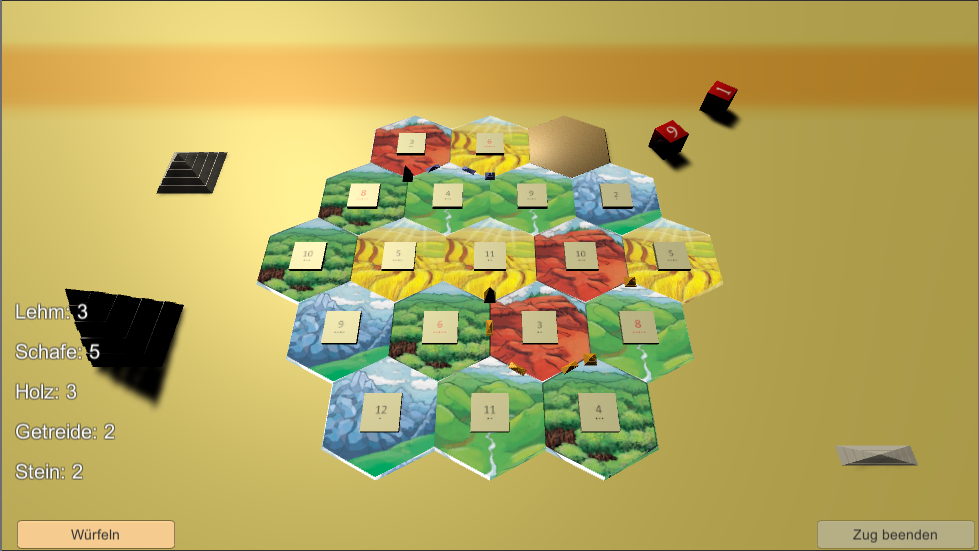
\includegraphics[height=8cm]{Bilder/AlleObjekte.png}
	\caption{Bau von St�dten, Siedlungen und Stra�en (eigene Darstellung)}
	\label{fig:AlleObjekte}
\end{figure}

Die n�chste Anforderung handelt von der Ermittlung eines Gewinners am Ende des Spiels. Diese wurde umgesetzt, indem jeder Spieler �ber eine Anzahl an Siegpunkten verf�gt. Wenn diese einen bestimmten Wert (Standard: 10) erreicht haben, so gilt das Spiel als beendet und der Spieler, der diesen Wert zuerst erreicht hat, wird auf dem GameOver-Bildschirm als Gewinner ausgegeben. Au�erdem ist auf diesem Bildschirm ein Button zu sehen, der den Start eines neuen Spiels erm�glicht. Im Hintergrund werden zudem alle Handlungen gestoppt und zur�ckgesetzt, sodass bei einem Neustart auch wirklich ein neues Spiel beginnt. Der GameOver-Bildschirm ist in Abbildung \ref{fig:GameOverScreen} zu sehen. 

\begin{figure}[h]
	\centering
	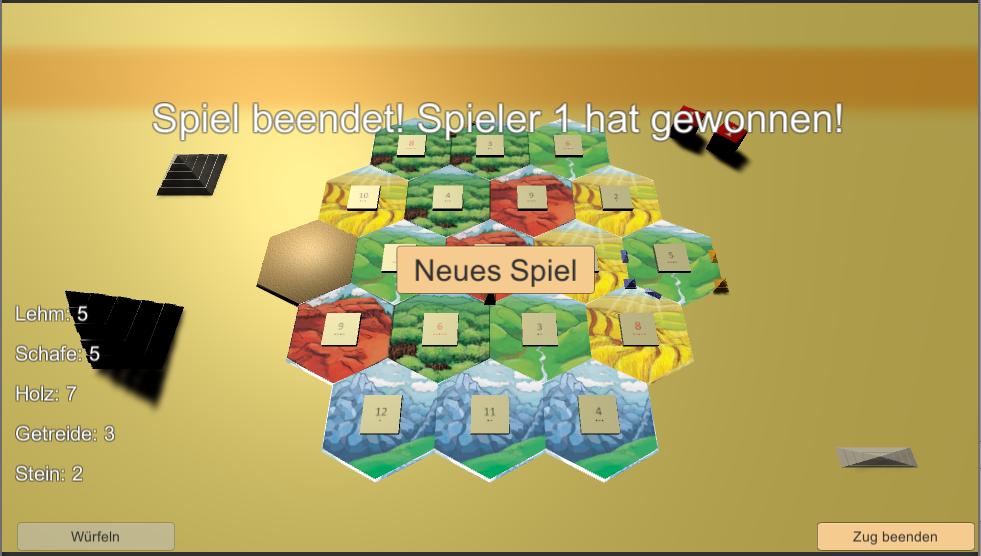
\includegraphics[height=8cm]{Bilder/GameOverScreen.png}
	\caption{Ausgabe des Gewinners auf dem Bildschirm (eigene Darstellung)}
	\label{fig:GameOverScreen}
\end{figure}

Da Siedler von Catan ein rundenbasiertes Spiel ist, muss im Spiel jedem Spieler ein Zug pro Runde zugeschrieben werden. In den Anforderungen wurde unter sechstens gefordert, dass ein solcher Zug immer mit dem W�rfeln beginnt, nachdem die Ressourcen verteilt werden und anschlie�end soll der Spieler bauen k�nnen. Diese Anforderung wurde genau so im Spiel umgesetzt. Zun�chst muss der Spieler den W�rfelbutton bet�tigen, ansonsten kann er keine andere Aktion ausf�hren. Erst danach ist es ihm m�glich weitere Aktionen auszuf�hren. Bezogen auf das Bauen, ist dies nur m�glich, wenn der Baumodus durch den Spieler aktiviert wird und dies wird wiederum nur erlaubt, wenn er gen�gend Ressourcen f�r den gew�hlten Baumodus hat. So muss der Spieler zum Bau von Stra�en beispielsweise mindestens ein Lehm und ein Holz besitzen. Diese beiden Abfragen sind relativ deutlich, doch kann auch der Fall auftreten, dass die Voraussetzungen zwar erf�llt sind, aber der Spieler dennoch keinen Bau ausf�hren kann. Dieser Fall kann zum Beispiel auftreten, wenn kein geeigneter Bauplatz zur Verf�gung steht. Dies kann auftreten, wenn bereits alle Siedlungen zu St�dten aufgewertet wurden und der Spieler dennoch den entsprechenden Modus aktiviert. In solch einem Fall,  wird keine weitere Stadt errichtet, denn der Baumodus aktiviert lediglich die Baupl�tze und diese sind bereits alle gel�scht, weshalb es hier zu keinem Problem kommt. Somit ist auch diese Anforderung komplett erf�llt.

Neben den notwendigen Anforderungen, die das Spiel erst erm�glichen, gibt es auch Regeln, die zwar zum Spiel geh�ren, aber keine Voraussetzung zum Spielen darstellen. Eine dieser Anforderungen ist die siebte. Diese besagt, dass zwischen St�dten bzw. Siedlungen mindestens zwei Stra�en liegen m�ssen. Implementiert wurde dies, indem die direkt an eine Siedlung oder Stadt angrenzenden Baupl�tze f�r weitere Siedlungen gel�scht werden. In der Praxis erfolgt dies, indem ein Vektor um eine Siedlung oder Stadt gelegt wird und jeder Bauplatz f�r Siedlungen im Umkreis entfernt wird. 
Dies l�st jedoch nur einen Teil des Problems. Abgesehen von den ersten beiden Z�gen darf der Spieler eine Siedlung nur an eine bereits bestehende gebaute Stra�e gebaut werden. Hierzu macht sich das Spiel erneut Entfernungen durch Vektoren zunutze. Denn wenn ein Baumodus aktiviert wird, aktiviert dieser nicht zwangsl�ufig alle Baupl�tze, die nicht gel�scht wurden. Stattdessen aktiviert der entsprechende Baumodus f�r Stra�en oder Siedlungen nur solche Pl�tze, die direkt an eine bereits bestehende Stra�e angrenzen. 
Beide Varianten kombiniert, erf�llen insgesamt die Anforderung, weil keine Baupl�tze nah genug an bestehenden Siedlungen existieren und gleichzeitig Stra�en sowie Siedlungen nur direkt an Stra�en gebaut werden k�nnen. Zudem gilt f�r St�dte das Gleiche wie f�r Siedlungen, da ein Bauplatz f�r eine Stadt nur dort errichtet wird, wo schon eine Siedlung steht. Dadurch wird �brigens auch die Anforderung acht erf�llt, die fordert, dass das Aufwerten von Siedlungen von Siedlungen auf St�dte im Spiel enthalten sein muss. 

Die Umsetzung der letzten Muss-Anforderung stellt auch gleichzeitig die komplizierteste Implementation dar. Denn hier wird gefordert, dass das Spiel berechnet, welcher Spieler die l�ngste Stra�e errichtet hat und dass dieser entsprechend mit Siegpunkten belohnt wird. Eine Stra�e in Siedler von Catan ist so definiert, dass einzelne aneinander liegende Stra�en eine l�ngere Stra�e bilden. Eine Stra�e aus einem St�ck hat somit die L�nge eins. Jedes weitere St�ck der Stra�e, dass direkt angrenzt, erh�ht die L�nge um ebenfalls um eins. Nach dieser Regel ist es somit auch m�glich eine Kreuzung zu errichten. Eine solche Kreuzung hat demnach die L�nge von drei und nicht von zwei. Die Umsetzung dessen erscheint zun�chst schwieriger als die der anderen Anforderungen zu werden, l�sst sich aber mit bereits bekannten Methoden implementieren. Denn die Vektoren aus Unity sind hier wieder von Nutzen. Konkret verf�gt jede Stra�e auf dem Spielfeld �ber einen Punkt im Raum, dessen Vektor zur Bestimmung der Entfernung zu anderen Stra�en (wie bei den Baupl�tzen) genutzt werden kann. Hierzu muss f�r jeden Spieler eine Pr�fung aller seiner Stra�en erfolgen. Im Quelltext dienen hierzu zwei Schleifen, die �u�ere durchl�uft alle Stra�en des Spielers und in der inneren wird jede Iteration gepr�ft, ob eine Stra�e im Einzugsgebiet liegt. Gleichzeitig sorgt ein rekursives Vorgehen daf�r, dass diese Stra�e ebenfalls als Ausgangspunkt genutzt wird. Jede Rekursion wiederum liefert die L�nge der Stra�e bis jetzt zur�ck. Somit ergibt die Tiefe der Rekursion die L�nge einer Stra�e. Da durch das Durchlaufen aller Stra�en zum Schluss jede Stra�e als Beginn genutzt wurde, ist sichergestellt, dass eine der bestimmten L�ngen die l�ngste Stra�e beschreibt und wenn das Maximum dieser L�ngen nun mit dem der anderen Spieler verglichen wird, kann die l�ngste Handelsstra�e dem passenden Spieler zugewiesen werden, wodurch die Anforderung erf�llt ist. 

Aufgrund der obigen Evaluation l�sst sich feststellen, dass alle Muss-Anforderungen, die gestellt wurden, erf�llt sind. Dadurch sind im folgenden Abschnitt die Soll- und Kann-Anforderungen zu bewerten. Hier war es nicht das Ziel alle zu erf�llen, sondern nur eine oder einige, um das Produkt �ber die Mindestanforderungen hinaus aufzuwerten. 

\section{Soll- und Kann-Anforderungen}
Die nicht erf�llten Anforderungen lassen sich schnell aussortieren. So wurde die Funktion von Ereigniskarten und das Ausspielen dieser Karten nicht implementiert. Auch der Dieb, der Ressourcen blockiert und deren Diebstahl erm�glicht, erhielt keinen Einzug ins Spiel. Zudem werden auch keine Gewinnwahrscheinlichkeiten ausgeben, auch der Handel zwischen Spielern oder mit der Bank ist nicht m�glich und es d�rfen auch maximal zwei Spieler gleichzeitig das Spiel spielen. Die damit ganz oder teilweise erf�llten Bedingungen belaufen sich damit auf die �brigen, die wie folgt umgesetzt wurden. 

Es ist m�glich, dass reale Spieler das Spiel spielen. Hierzu muss nur eine Einstellung zu Beginn des Spiels im Startmen� vorgenommen werden. Diese ist schon so implementiert, dass auch die n�chste Anforderung, die einen KI-Spieler und einen realen Spieler erm�glichen soll, erf�llt wird. Denn f�r Spieler 1 und Spieler 2 kann jeweils ein Haken (KI an) gesetzt werden. Ist das K�stchen ausgew�hlt, so wird der entsprechende Spieler durch die KI gesteuert, ansonsten muss ein menschlicher Spieler die Z�ge ausf�hren. 

Dar�ber hinaus gilt eine weitere Kann-Anforderung als erf�llt: Es werden initiale KIs bereitgestellt. In Abschnitt \ref{sec:InitialeKI} wird darauf n�her eingegangen. Daher wird dieser Punkte hier verk�rzt behandelt werden. Es bleibt lediglich zu auszusagen, dass diese KIs grundlegende Strategien verfolgen und diese auch �ber das Spiel hinweg gleich bleiben. So �ndert die KI beispielsweise nicht ihre Strategie, wenn sie nur noch wenige Siegpunkte braucht, wobei dies nat�rlich durch eine Erweiterung der Fallbasis m�glich w�re. Durch die Bereitstellung der initialer F�lle und der Gewichtung von Attributen sind jedoch erweiterbare KIs Teil des Produktes geworden, bei denen nun die Fallbasis ausgetauscht oder erweitert werden kann, was f�r intelligenteres Verhalten sorgen kann. Sie unterscheiden sich damit fundamental von denen in Abschnitt \ref{sec:InitialeKI} beschriebenen Testreaktionen der KI. 

\section{Anforderungen an die Schnittstelle}
Neben direkten Anforderungen an das Spiel an sich wurden auch spezielle an die Schnittstelle gestellt, die die Qualit�t weiter steigern sollen. 

Bei der ersten wird gefordert, dass die KIs ohne gro�en Aufwand ausgetauscht werden k�nnen m�ssen. Dies ist durch die fallbasierte Umsetzung der initialen KIs erm�glicht. Die Fallbasis kann einfach in der Projektdatei angepasst werden. Lediglich die Standardf�lle sind durch den Quelltext abgedeckt. Hieran also beliebig angepasst und ausgetauscht werden, was die Anforderung erf�llt. 

Die zweite Anforderung sagt aus, dass die KIs in unterschiedlichen Programmiersprachen umgesetzt sein d�rfen. Dieser Punkt ist kein Teil der Standardumsetzung und wurde auch nicht im Detail verfolgt. Allerdings kann er dennoch als erf�llt betrachtet werden, denn als Kommunikationsmittel wird JSON benutzt. Wenn nun zus�tzlich im Quellcode des Spiels das aufgerufene Programm ausgetauscht wird, so kann auch eine andere Programmiersprache die Rolle von \textit{CBRSystem.jar} �bernehmen. 

Die n�chste Anforderung wurde schon beim Beschreiben der Anforderungen f�rs Spiel mitbetrachtet. Da zum Start der Spiels ausgew�hlt werden kann, ob Mensch-Mensch, Mensch-KI oder KI-KI gegeneinander spielen,muss die Schnittstelle zwangsl�ufig das Antreten von zwei computergesteuerten Spielern erm�glichen. 

Die letzte Anforderung erfordert erneut den gr��ten Erl�uterungsbedarf. Diese m�chte n�mlich, dass die KI einem menschlichen Spieler gegen�ber weder bevorteilt oder benachteiligt wird, was durchaus vorkommen k�nnte. Hierf�r ist n�mlich entscheidend, dass Mensch und Maschine die gleichen Informationen erhalten, obwohl sie nicht �ber die gleiche Wahrnehmung verf�gen. Die KI muss also eine Situationsbeschreibung erhalten, die dem gleicht, was ein menschlicher Spieler auf dem Spielfeld sehen w�rde, wenn er dran ist. Au�erdem ist der Zeitpunkt der Informations�bermittlung relevant, weil kein konstanter Fluss erfolgen kann, wie bei der Betrachtung eines Bildschirms durch einen Menschen. Somit sollte die KI immer dann eine neue Situationsbeschreibung erhalten, wenn sie am Zug ist und die Situation so deutlich ge�ndert hat, dass davon auszugehen ist, dass sie andere Aktionen ausf�hren m�chte, als sie vorher ausgew�hlt hat. In der Implementation wird dies umgesetzt, indem zum Beginn eines Zuges eine Anfrage, die eine Situationsbeschreibung enth�lt, an die KI geschickt wird. Auf diese kann sie mit einem Plan reagieren. Dieser besteht aus einer Liste von Anweisungen, die die KI ausf�hren m�chte. Das Spiel f�hrt die Aktionen nach und nach im Namen des Spielers aus, sofern dies m�glich ist. Wenn alle Aktionen ausgef�hrt wurden, wird die neue Situation der KI erneut �bermittelt und sie kann weitere Aktionen durchf�hren. Dies geschieht so lange, bis im Plan der Wunsch nach dem Beenden des Zuges auftritt. Hierdurch endet der Zug der KI sofort und der n�chste Spieler ist an der Reihe. Einen Ausnahmefall stellt ein leerer Plan dar. Wenn die KI auf eine gegebene Situation keine Antwort wei�, so kann es vorkommen, dass sie eine leere Antwort sendet. Dieser Fall wurde in Abschnitt \ref{sec:Staedte} schon im Detail beschrieben. Das dort beschriebene Vorgehen gew�hrleistet, dass durch einen Fehler der KI, ihr Zug nicht abrupt beendet wird. Stattdessen erh�lt Sie erneut die Chance auf die gegebene Situation angemessen zu reagieren. Antwortet sie allerdings weiterhin unsinnig, so wird ihr Zug dennoch beendet und der n�chste Spieler ist an der Reihe. 

Allgemein kann durch dieses Vorgehen die gleiche Informationsverf�gbarkeit simuliert werden, die auch einem Menschen zug�nglich w�re. Zwar kann der Mensch dauerhaft auf seine Rohstoffe schauen, das Spielgeschehen auf der Spielfeld im Blick behalten und seine Strategie �ndern und die KI ist dazu nicht in der Lage, doch muss dies auch nicht der Fall sein. Es reicht wenn die KI ihre Handlungen bei einer Situations�nderung �berdenken darf. Denn der Mensch wird seine Strategie wahrscheinlich auch nur dann �berdenken, wenn sich etwas an seiner Situation �ndert. F�r die KI wurde dies �quivalent umgesetzt. Zu Beginn eines Zuges darf die KI ihren Zug planen und nach Ausf�hrung des Plans eventuell einen neuen umsetzen. Hierdurch l�sst sich insgesamt schlie�lich, dass die genannte Anforderung an die Schnittstelle erf�llt wurde und ein Grundsatz von Fairness zwischen dem menschlichen und dem computergesteuerten Spieler etabliert wurde. 

Zu den Soll- und Kann-Anforderungen an die Schnittstelle bleibt festzuhalten, dass diese im gleichen Umfang umgesetzt wurden, wie sie den umgesetzten Anforderungen an das Spiel dienen. 

Abschlie�end kann aufgrund der obigen Analyse die Aussage getroffen werden, dass auch f�r die Schnittstelle alle n�tigen Anforderungen hinreichend umgesetzt wurden. Lediglich an der Verwendung anderer Programmiersprachen au�er Java und C\# zur Implementierung weiterer KIs Bedarf es an mehr Aufwand. Hierbei bleibt aber dennoch zu sagen, dass es m�glich ist, sofern die Schnittstelle JSON genutzt wird und das angesteuerte Programm im Quellcode des Spiels vermerkt wird.

%\section{Aufgetretene Probleme}
%Viele Softwareprojekte laufen nicht so ab, wie es zuvor geplant wurde. H�ufig treten Probleme auf, die vorher nicht bedacht wurden und dann die Entwicklung verz�gern oder sogar zu einer angepassten Funktionsweise f�hren. Dies war auch im Rahmen der Entwicklung der Software zu dieser schriftlichen Ausarbeitung der Fall. Einige Hindernisse traten auf, die zun�chst einmal bew�ltigt werden mussten, bevor andere Funktionalit�ten in Betracht gezogen wurden. In diesem Abschnitt sollen diese Probleme behandelt und auch deren L�sung kurz erl�utert werden. Dabei wird selbstverst�ndlich nicht auf jeden einzelnen Fehler eingegangen, der w�hrend der Entwicklung auftrat, aber auf alle gr��eren Hindernisse. Zun�chst sollen solche behandelt werden, die gel�st wurden. Anschlie�end auch auf die, die bestehen bleiben.

\section{Behobene Probleme}

Die Integration der KI und insbesondere der Schnittstelle erwies sich aufgrund des eigenen Vorgehens als schwierig. Hier h�tten r�ckblickend wahrscheinlich mehrere Stunden eingespart werden k�nnen. Denn zun�chst konzentrierte ich mich nur auf eine laufende Version des Spiels. Es wurde v�llig vernachl�ssigt, wie die Schnittstelle und damit auch die KIs sp�ter noch eingebunden werden k�nnen. Hierdurch entstanden vor allem konzeptionelle Hindernisse. Da das Spiel anfangs nur auf menschliche Spieler ausgelegt war, konnten diese zwar spielen, aber der eigentliche Sinn, KIs gegeneinander antreten zu lassen, r�ckte in den Hintergrund. Daraus resultierend wuchsen Klassen von MonoBehaviour erbend. Sie �bernahmen auch Funktionalit�ten, die auch in eine andere Klasse h�tten ausgelagert werden k�nnen. Hier h�tte sich eine h�her gelagerte Klasse \textit{Spieler} angeboten. Diese h�tte alle allgemeinen Eigenschaften des Spielers �bernommen und in der Klasse \textit{PlayerScript} h�tten lediglich Funktionen, die Unity direkt betreffen, vorhanden sein m�ssen. Stattdessen sind �bergeordnete Funktionen jetzt auch in die PlayerScript-Klasse integriert, was w�hrend der Programmierung f�r kleinere Probleme sorgte. An sich bietet es jedoch auch Vorteile. So erfolgt die Verwaltung des Spielers an einer zentralen Stelle im Spiel und �nderungen an den Attributen der Entit�t eines Spielers durch die KI wirkt sich genau so aus, als w�ren die �nderungen durch einen Menschen vorgenommen worden. Dies kommt dem Aspekt der Fairness wiederum zugute. 

Insgesamt zieht sich dieses Vorgehen durch die gesamte Schnittstelle. Die Klasse \textit{PlayerScript} dient hierbei nur als gr��tes Beispiel. Andere F�lle in denen dieses Vorgehen deutlich wird, sind die abstrakten Baupl�tze, die teilweise direkt in den Entit�ten des Spiels erzeugt werden, um sie dann an die KI zu schicken. Auch dies scheint konzeptionell fragw�rdig, liefert aber eine enge Verzahnung beider Spielmodi (Mensch vs. KI). 

Durch eine l�ngere bzw. bessere Konzeptionsphase h�tte ich das ungewollte auftreten solcher Verzahnungen wohl m�glich verhindern oder zumindest den Einsatz auf gewollte Male beschr�nken k�nnen. Wie gro� der Einfluss auf die Dauer des Projektes im Endeffekt genau war, l�sst sich nur schwer beziffern. Auf der einen Seite ist der Quellcode auf diese Weise m�glicherweise schlechter nachzuvollziehen, was bei �nderungen zu einer Verz�gerung f�hren kann. Andererseits h�tte die Konzeption auch mehr Zeit in Anspruch nehmen m�ssen. Diese beiden Aspekte gilt es also gegeneinander abzuw�gen. Langfristig kann jedoch ausgesagt werden, dass dann ein Zeitersparnis durch die Konzeption entsteht.

Auch die Implementierung von Testreaktionen h�tte besser konzipiert werden k�nnen und h�ngt eng mit dem obigen Aspekt zusammen. Damit die KI sinnvoll agieren kann, muss zun�chst einmal eine geeignete Situationsbeschreibung erstellt werden, die dann mittels JSON �ber die Schnittstelle der KI zug�nglich gemacht wird. Durch das Implementieren der Schnittstelle, nachdem bereits eine laufende Version f�r menschliche Spieler erstellt wurde, erwies sich auch das als Hindernis. Zur L�sung wurde zus�tzlich zu jedem relevanten Unity-Objekt eine abstrakte Darstellung in Form einer Klasse erzeugt, die alle relevanten Informationen enth�lt. Die Zusammenfassung dieser Klassen in Form der Klasse \textit{Situation} erm�glichte schlie�lich eine geeignete �bermittlung der Daten, sodass die KI antworten kann. 

Zu diesem Zeitpunkt unterst�tzte die KI jedoch noch keine wirklich intelligente Verwaltung von Wissen. Stattdessen musste im Quellcode mittels Verzweigungen festgehalten werden, wie auf bestimmte Eigenschaften einer Situation reagiert wird. Dies vereinfachte das Testen des Spiels und half dabei, die Schnittstelle richtig zu konfigurieren. Dennoch erschwerte dies das Einf�hren der fertigen bzw. initialen KI. Diese arbeitet fallbasiert mit dem MyCBR zusammen und hierf�r mussten wieder fundamentale �nderungen am Quellcode vorgenommen werden. Die Anpassungen an der Schnittstelle waren minimal. Lediglich die Java-Klasse \textit{CBRSystem} musste etwas umgebaut werden. Doch war die �berf�hrung der Situation in Form einer Klasse in F�lle, die die Fallbasis versteht, relativ aufwendig. Au�erdem �nderte ich die Fallbasis zur Erh�hung der Intelligenz der KI dauerhaft. Auch dies war mit hohem Anpassungsaufwand verbunden. 

R�ckblickend w�rde ich auch dies anders l�sen. Ich w�rde zun�chst genau festlegen, welche Reaktionen eine initiale KI zeigen soll und dann F�lle definieren, mit denen diese Reaktionen erreicht werden kann. Somit w�rde die Implementation von Testreaktionen ohne Fallbasis wegfallen und es w�re mehr Zeit zur Verbesserung der initialen KIs geblieben. Kombinieren w�rde ich dieses Vorgehen mit dem oben beschriebenen Punkt, der besagt, dass mehr Zeit auf die Konzeption h�tte verwendet werden sollen. Dann w�re das Spiel zwar langsamer und mit zun�chst weniger Features, aber daf�r insgesamt schneller entstanden und die weitere Funktionalit�ten h�tten mit weniger Aufwand Einzug ins Spiel erhalten k�nnen. 

Das Stoppen des Spiels war bevor die KIs eingef�hrt werden auch kein Problem. Der Gamemanager wurde disabled, was automatisch dazu f�hrte, dass das Spiel nicht weitergef�hrt werden konnte. Die Anfrage durch das Spiel an die Schnittstelle erfolgt allerdings unabh�ngig von der Update-Methode des Gamemanagers, was zu einem Fortf�hren des Spiels f�hrt, selbst wenn schon der \textit{Game Over Screen} angezeigt wird. Um dieses Problem zu beheben wurde, vor dem Starten einer Anfrage an die KI getestet, ob nicht schon ein Spieler gewonnen hat. Sollte dies der Fall sein, wird keiner weitere Anfrage gesendet und das Spiel stoppt. Eigentlich handelt es sich hierbei mehr um einen einfachen Bug, als um ein Problem, das die Umsetzung betrifft. Allerdings geht es in die gleiche Richtung wie die oben aufgef�hrten und wird daher auch in diesem Zusammenhang behandelt. 

Das Vorherbestimmen der Antworten der fertigen KI erwies sich als weiteres Problem. Hierbei wurden zwar Standardf�lle in die Fallbasis eingef�gt, die f�r ein bestimmtes Verhalten der KIs sorgen sollten. Die KIs verhielten sich allerdings nicht immer wie erwartet. Sodass schlie�lich einige Einschr�nkungen in das Retrieval eingef�hrt und eine Erweiterung der Fallbasis vorgenommen werden musste. 

Ein Beispiel f�r einen solchen Fall ist das Einbeziehen des vorherigen Plans der KI in die aktuelle Entscheidung. Dies w�re n�tig, wenn Baupl�tze f�r Siedlungen aktiviert werden sollen. Es kann vorkommen, dass die KI den Plan, Baupl�tze zu aktivieren entsendet, aber keiner aktiviert wird. Dann h�tte sich die Situation f�r die KI nicht ge�ndert und sie w�rde diesen Plan immer wieder entsenden. In der Implementation wird dieses Problem nun gel�st, indem der vorherige Plan zwischengespeichert wird und mit dem aktuellen abgeglichen wird. Somit kann ein Fehlverhalten verhindert und ein alternatives Vorgehen in die KI integriert werden. Allerdings w�re es angebracht auch dies fallbasiert zu l�sen. Hierzu wird die Situation an sich ver�ndert. Hierf�r musste pro Aktivierungsaktion eine Methode zur Verf�gung gestellt werden, die einbezieht, ob es �berhaupt aktivierbare Pl�tze gibt. Diese Information wird in Form eines weiteren Symptoms in den F�llen gespeichert. Konkret handelt es sich dabei um drei Symptome, die mit Wahrheitswerten zu f�llen sind, pro Bauplatzart einer.

Am simpelsten ist die �berpr�fung von St�dtebaupl�tzen. Hierf�r pr�ft die entsprechende Methode lediglich, ob der aktuelle Spieler �ber Siedlungen verf�gt, denn jede Siedlung ist auch gleichzeitig ein Bauplatz f�r eine Stadt. Wenn also unausgebaute Siedlungen auf dem Spielfeld vorhanden sind, so k�nnen auch St�dtebaupl�tze aktiviert werden. 

Schwieriger gestaltet sich die �berpr�fung f�r Stra�en und Siedlungen. Hierf�r muss das Spiel diese Information direkt mit in die Situation einf�gen. Hierzu wurde eine Methode gestaltet, die eine normale Aktivierung der Pl�tze simuliert und speichert, wie viele Aktivierungen vorgenommen wurden. Im Fall von null Aktivierungen w�rde ein \textit{false} ansonsten ein \textit{true} �bermittelt werden. Dies ist f�r Stra�en und Siedlungen �quivalent einsetzbar. Zu beachten ist, dass hierdurch das Spiel eine erbringt, die eigentlich durch die KI selber erbracht werden m�sste. Schlie�lich muss ein menschlicher Spieler auch selbst feststellen, dass ein erneutes Dr�cken des Buttons zum Aktivieren von Baupl�tzen unsinnig ist, wenn beim ersten Versuch, schon keine Pl�tze aktiviert wurden. Der Grundsatz der Fairness k�nnte hierdurch zwar als verletzt betrachtet werden jedoch nur theoretisch. In der Praxis ist das Erkennen der gleichen Handlung als unsinnig so grundlegend, dass die KI dadurch nicht bevorteilt wird. 

Abschlie�end bleibt zu den behobenen Problemen zu sagen, dass diese zwar einen Einfluss auf die Umsetzung des Projektes hatten und durch eine bessere Konzeption m�glicherweise Zeit h�tte gespart werden k�nnen. Jedoch hielten die aufgef�hrten Hindernisse das Fortschreiten der Entwicklung nicht solch einem Ausma� zur�ck, dass der Erfolg der Implementierung zu einem Zeitpunkt gef�hrdet gewesen w�re. Denn an sich wurde viel Zeit in die Konzeption gesteckt, was im Kapitel \ref{cha:Entwurf} Entwurf nachzulesen ist. In der tats�chlichen Umsetzung mussten dann aber Anpassungen vorgenommen werden, die einige Aspekte des Entwurfs hinf�llig machten. Eventuell w�re es daher eine Option gewesen, wenn deutlich wird, dass ein Aspekt nicht so umgesetzt werden kann, zur�ck zum Entwurf zu gehen und diesen zu �berarbeiten. Hierdurch h�tten die genannten unerw�nschten Effekte vermieden werden k�nnen. 

\section{Tests}
\label{sec:Tests}
Zur genaueren Evaluierung der Software wurden 20 Testspiele durchgef�hrt, bei denen jeweils beide Spieler KI-Spieler waren. Die angewendeten Strategien sind unter Abschnitt \ref{sec:InitialeKI} nachzulesen. Genau genommen, versucht Spieler eins Ressourcen zu gewinnen, um St�dte zu bauen und Spieler 2 konzentriert sich auf n�tige Ressourcen f�r Siedlungen und Stra�en. 

Nach 20 Spielen hatte Spieler 1 sechs Siege zu verzeichnen, Spieler 2 sieben und bei weiteren sieben Spielen kam es zu keiner finalen Entscheidung, weil die Spieler entweder nicht alle Ressourcen erlangten oder sie sich gegenseitig so eingebaut haben, dass keiner mehr den Sieg erlangen konnte. Eine Visualisierung der Ergebnisse ist in Abb. \ref{fig:Ergebnisse} zu sehen. 

\begin{figure}[h]
	\centering
	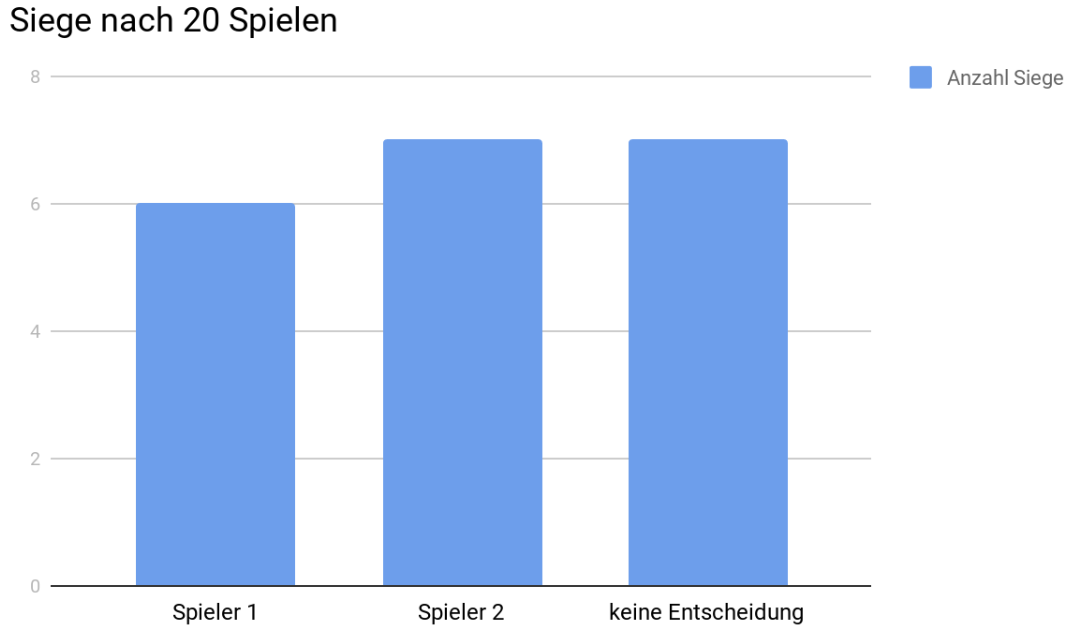
\includegraphics[height=9cm]{Bilder/Testergebnisse.png}
	\caption{S�ulendiagramm zu den Testergebnissen (eigene Darstellung)}
	\label{fig:Ergebnisse}
\end{figure}

Mithilfe dieser Ergebnisse lassen sich Probleme identifizieren, die noch nicht behoben wurden und einen Grundstein f�r sp�tere Verbesserungen legen. 

\textbf{Die Strategien sorgten f�r keinen signifikanten Unterschied im Ergebnis:}\\
Da Spieler 1 sechs mal gewann und Spieler 2 sieben der 20 Spiele, scheint die Strategie keinen oder zumindest keinen gro�en Einfluss auf das Ergebnis zu haben. M�glicherweise sind beide Strategien ungef�hr gleich gut oder das Pr�ferieren eines Rohstoffs wirkt sich nicht allzu stark aus. 
\\\\
\textbf{Spieler erlangen nicht immer alle n�tigen Ressourcen:}\\
Von den gespielten 20 Spielen konnten ganze sieben nicht zu Ende gespielt werden, weil keiner mehr eine Chance auf den Sieg hatte. Bei sechs dieser Spiele war der Grund. dass zu Beginn des Spiels keiner der Spieler Zugang zu allen n�tigen Ressourcen erlangte. Ohne die M�glichkeit zum Handeln muss jeder Spieler seine ersten beiden Siedlungen so platzieren, dass er mindestens Zugang zu Lehm, Holz, Schafen und Getreide hat. Diese Ressourcen sind n�tig, um neue Siedlungen bauen zu k�nnen und ohne diese ist kein Sieg m�glich. 
\\\\
\textbf{Der W�stenbug trat auf:}\\
In ca. einem von 19 F�llen wird die Mitte des Spielfelds als W�ste gew�hlt, wenn dies geschieht, wird ein leeres Prefab f�r Nummern dort platziert. Dies sollte nicht vorkommen, beeinflusst das Spielgeschehen an sich jedoch nicht. 
\\\\
\textbf{Spieler k�nnen sich gegenseitig einbauen:}\\
Der �brige Fall, der f�r ein Spiel ohne Sieger sorgte, ist durch gegenseitiges Einbauen zu erkl�ren. Es kann vorkommen, dass einer oder beide Spieler vermehrt Stra�en bauen, weil andere Ressourcen Ihnen gerade nicht zur Verf�gung stehen. Dadurch wird in einigen Spielen, dass gesamte Spielfeld durch Stra�en belegt und es bleibt kein freier Platz. Die aktuellen KIs Wissen nicht, wie auf eine solche Situation zu reagieren ist und stellen das Handeln ein. Dies f�hrt dazu, dass ein Spiel, welches theoretisch noch beendet werden k�nnte, aufgrund der Intelligenz der KI keinen Sieger findet.

Abschlie�end bleibt zu den identifizierten Problemen zu sagen, dass innerhalb der 20 Spiele keine Situation auftrat, auf die die Spieler anders als erwartet reagierten. Es kam demnach nicht zu Fehlern, die einen Spielabbruch zur Folge gehabt h�tten. Hierdurch kann nun zumindest vermutet werden, dass die Software sicher l�uft und f�r eine Einhaltung der geltenden Spielregeln sorgt. Au�erdem haben auch alle Funktionalit�ten wie erwartet funktioniert. Die beschriebenen Probleme h�ngen haupts�chlich mit der Intelligenz der KI zusammen und nicht mit dem Spiel an sich. 







\chapter{Fazit \& Ausblick}
Ziel dieser Arbeit war es ein rundenbasiertes Strategiespiel f�r K�nstliche Intelligenz spielbar umzusetzen und die Konzeption, Implementation und Evaluation zu dokumentieren. Konkret wurde dabei das bekannte Gemeinschaftsspiel \quotes{Siedler von Catan} als Ziel der Implementation gew�hlt. 

Die Arbeit an sich war in mehrere Kapitel unterteilt. So wurde zun�chst in Kapitel 1 das Thema eingeleitet und beschrieben, wovon die Arbeit handeln wird. Das zweite Kapitel befasste sich anschlie�end mit den zum Verst�ndnis der �brigen Arbeit n�tigen Grundlagen. Danach wurde sich in Kapitel 3 das erste Mal mit der entstehenden Software besch�ftigt. Hier wurde im Detail die Konzeption erl�utert, die sich wiederum in die Problemstellung und den konkreten Entwurf aufteilen l�sst. Nachdem die Konzeption abgeschlossen wurde, folgt die Implementation des beschriebenen in Kapitel 5. Dieses beschreibt von den ersten Schritten bis zur fertigen Software alle wichtigen Aspekte der Umsetzung. Eine Unterteilung erfolgt innerhalb des Kapitels in Abschnitte �ber das Spiel selbst, die Schnittstelle und die Implementierung von initialen KIs. Au�erdem erfolgt noch eine Betrachtung der Anpassungen, die im Vergleich zum Entwurf vorgenommen wurden. Mit Kapitel 6 f�gt sich die Evaluation an. Diese befasst sich zun�chst einmal mit den Muss-Anforderungen und bewertet, ob alle erf�llt wurden. Im weiteren Verlauf des Kapitels wird auf die Kann- bzw. Soll-Anforderungen eingegangen. Auch wird gepr�ft, welche dieser Anforderungen umgesetzt wurden und wie sich die Umsetzung weiterer Anforderungen auswirken w�rde. Nachdem die Anforderungen an das Spiel �berpr�ft wurden, wird auf die an die Schnittstelle �bergegangen. Neben der �berpr�fung von Anforderungen werden in der Evaluation auch Tests betrachtet und Schl�sse gezogen, wie die KIs abgeschnitten haben. Abgeschlossen wird das Kapitel durch eine Betrachtung von Problemen, die w�hrend der Entwicklung aufgetreten sind. Hierbei wird zwischen behobenen und andauernden unterschieden. 

\section{Fazit}
Die angefertigte Software und diese schriftliche Ausarbeitung beschreiben nicht die komplette Umsetzung des Spiels \quotes{Siedler von Catan} mit allen Details. Stattdessen wurden aus den Spielregeln die wichtigsten Aspekte extrahiert und als Anforderungen formuliert. Diese dienen als Grundlagen, um den Erfolg des Projektes bewerten zu k�nnen. Wie im oberen Absatz bereits erw�hnt, wurde die Erf�llung dieser Anforderungen in der Evaluation �berpr�ft. Hierbei wurde deutlich, dass alle Muss-Anforderungen umgesetzt wurden und auch ein gro�er Teil der Kann- bzw. Soll-Anforderungen. Dadurch ergibt sich insgesamt, dass der Umfang des Spiels im Vergleich zur Brettspielvariante etwas reduziert wurde, aber dennoch ein funktionierendes, in sich stimmiges Produkt geschaffen wurde. Der Umfang ist in sofern beschr�nkt, indem der Handel und der Einsatz des R�ubers sowie Ereigniskarten nicht zur Verf�gung stehen. Stattdessen wurde sich auf initiale KIs fokussiert. Hierdurch konnte letztendlich erreicht werden, dass die Software bereits funktioniert und die KIs gegeneinander spielen k�nnen. 

Insgesamt ergibt sich auf diese Weise ein fertiges Produkt und das Ergebnis dieser Arbeit l�sst sich als Erfolg bezeichnen. An vielen Stellen im Verlauf des Projektes h�tte es zu Verz�gerungen kommen k�nnen, die die Implementierung des umgesetzten h�tten gef�hrden k�nnen. Dies war immer dann der Fall, wenn es zu unvorhergesehenen Problemen kam, wie solche, die in der Evaluation (Kapitel \ref{cha:Evaluation}) beschrieben werden. Der erfolgreiche Abschluss war jedoch zu keinem Zeitpunkt in Gefahr. Das h�ngt zum einen mit der Konzeption im Vorhinein und zum anderen mit der zeitlichen Planung zusammen. Es wurde bereits fr�h mit der Umsetzung begannen, sodass die schriftliche Arbeit und die Weiterentwicklung der Software gr��tenteils zeitgleich erfolgte. Besonders wichtig war hierbei, dass ich mich bereits mit Unity und C\# auseinander setzte, als ich die Konzeptionierung noch nicht fertig hatte. Dadurch konnte ich mein gewonnenes Wissen bereits in die Konzeption mit einflie�en lassen und diese genauer gestalten. Auch konnte ich die Entwicklung der Software vor der schriftlichen Ausarbeitung abschlie�en, wodurch weitere zeitliche Probleme verhindert werden konnten. 

Abgesehen von der zeitlichen Dimension und der Erstellung eines funktionierenden Produktes war das Projekt auch auf anderen Dimensionen ein Erfolg. Als Bachelorarbeit diente es als Abschluss des Studiums und im besten Fall flie�t m�glichst viel Wissen, das bis dort im Studium gewonnen wurde, in die Arbeit ein. Dies war hier der Fall. Im Verlauf des Studiums konnte ich mir Kenntnisse �ber Wissensbasierte Systeme und Softwareentwicklung aneignen. Auch die Erfahrung aus vorherigen Softwareprojekte konnte ich f�r mich nutzen, um die zeitlichen Ausma�e besser einzusch�tzen. Neben diesen F�higkeiten war es sicherlich auch von Vorteil, dass bereits eine Projektarbeit abgelegt werden musste, die auch zumindest zum Teil aus der Implementierung eines Algorithmus bestand. Dieses gewonnene Wissen trug zum erfolgreichen Abschluss der Entwicklung der Software und der schriftlichen Ausarbeitung bei. 

Selbstverst�ndlich musste f�r die erfolgreiche Entwicklung der Software und dem Abschluss des Projektes sich auch neues Wissen angeeignet werden. Hierbei sind allem voran der Umgang mit Unity und die Programmiersprache C\# zu nennen. Zwar kannte ich mich bereits in �hnlichen Sprachen wie Java und C++ aus, aber mit C\# hatte ich davor nur wenig Kontakt gehabt, geschweige denn ganze Projekte darin umgesetzt. Es half mir daher sehr, dass ich mich schon vor Projektbeginn mit C\# auseinandersetze und kleinere Projekte realisierte. So konnte ich letztendlich schneller das eigentliche Projekt umsetzen. Diese Lernzeit brauchte ich aber weniger zum Lernen der Programmiersprache an sich, sondern f�r den Umgang mit Unity. Mit Unity oder einer anderen Game-Engine hatte ich bis dato keinen Kontakte gehabt und musste mich daher v�llig neu darin einfinden. Ich kombinierte meinen Lernaufwand f�r C\# und Unity, indem ich direkt in Unity begann kleinere C\#-Projekte umsetzen. Diese halfen mir ein allgemeines Verst�ndnis �ber Scenes, Prefabs, Scripts und weitere Aspekte von Unity zu erlangen. Im Endeffekt stellte Unity die deutlich gr��ere H�rde als C\# dar, weshalb ich darauf auch mehr Zeit aufwendete. Nichtsdestotrotz stellten beide kein so gro�es Hindernis dar, dass sie eine erfolgreiche Umsetzung des Projektes h�tten verhindern k�nnen. 

Die Umsetzung des Spiels gestaltete sich dann auch nicht als allzu aufwendig. Es gab zwar einige Aspekte, die mit einem hohen Aufwand verbunden waren, aber im Allgemeinen waren Schnittstelle und initiale KI deutlich schwieriger umzusetzen. Hierbei erwies sich die M�glichkeit auf ein �hnliches, bereits abgeschlossenes Projekt zuzugreifen als gro�er Vorteil. Ich konnte mir die Arbeit von Jannis Hillmann ansehen und auch Aspekte seiner Programmierung �hnlich wiederverwenden. Er setzte ein �hnliches Projekt aber mit Grundlage eines Ego-Shooters um. Ich konnte durch das Nachvollziehen seiner Arbeit und der �bertragung dieses Wissens auf meinen Anwendungsfall enorm viel Zeit sparen. Wenn dieses Projekt nicht zur Verf�gung gestanden h�tte, dann w�re wahrscheinlich die Anfertigung von initialen KIs aus Zeitgr�nden k�rzer und damit weniger umfangreich ausgefallen. 

Abschlie�end l�sst sich, wie eingangs erw�hnt, das gesamte Projekt als Erfolg bezeichnen. Nicht nur wurden alle Muss-Anforderungen umgesetzt, es fanden sogar zus�tzliche Kann- und Muss-Anforderungen Einzug in die Implementation. Abgesehen davon konnte ich mein bereits im Studium erworbenes Wissen einsetzen und mit neuem kombinieren, was auch den praktischen Nutzen von theoretisch gelernten Inhalten darlegt. In Bezug auf den zeitlichen Rahmen konnten durch die Planung und die Einteilung Probleme vermieden werden. 

\section{Ausblick}
\label{sec:Ausblick}
Wie der Name dieses Abschnitts schon vermuten l�sst, sollen hier sowohl f�r die entwickelte Software als auch f�r die schriftliche Ausarbeitung Aspekte beschrieben werden, an denen weitere Arbeiten ansetzen k�nnen. Als gro�e Punkte sind hier das L�sen von bestehenden Problemen, der Handel zwischen Spielern, der Dieb und das Verwenden von Ereigniskarten zu nennen. Durch die Erweiterung des Spiels um diese Funktionen, w�rde das Spielen an sich eine komplexere Strategie erfordern bzw. eine bessere Performanz aufweisen. In

Wenn eine dieser Anforderungen implementiert w�rde, dann sollte am ehesten der Handel gew�hlt werden, da dieser die interessantesten strategischen Optionen bietet, indem er eine direkte Interaktion zwischen zwei Spielern erm�glicht. Hier m�sste die KI miteinbeziehen, dass der andere m�glicherweise auch profitiert und es muss abgewogen werden, ob die KI selbst mehr vom Handel profitiert als der Gegner dies tun w�rde. Diese Frage stellt sich sowohl als Initiator eines Handels als auch als sein Partner.

\subsection{Verbesserungen} 
Allgemein stellen alle geschilderten Probleme aus Abschnitt \ref{sec:Tests} Tests einen m�glichen Ansatz f�r Verbesserungen dar. 

So ist hier die L�sung des Bugs zu nennen, der auftritt, wenn die W�ste in der Mitte des Spielfelds erstellt wird. Dieser Bug hat keinen Einfluss auf das Spiel an sich, weshalb eine L�sung in kommenden Softwareerweiterungen m�glich, aber nicht notwendig ist. Jedenfalls muss zu seiner L�sung lediglich ein Weg gefunden werden, das Prefab auf dem mittleren Sechseck zu l�schen. Falls sich dies als zu aufwendig erweisen sollte, kann alternativ auch verhindert werden, dass die W�ste die Mitte belegt. 

Des Weiteren m�sste ein Vorgehen f�r den Fall entwickelt werden, dass ein oder beide Spieler keinen Zug mehr machen k�nnen. Beispielsweise wenn eine KI, weil sie von der anderen eingebaut wurde oder weil alle Baupl�tze bereits belegt sind, nichts mehr tun kann. In solch einem Fall k�nnte sie zwar ihren Zug beenden, aber an sich w�rde die andere KI ab diesem Zeitpunkt alleine spielen. Sie k�nnte nun solange weitermachen, bis sie genug Siegpunkte gesammelt hat. Andere L�sungen w�ren jedoch auch, der KI zu diesem Zeitpunkt den Sieg einfach zuzuschreiben, da f�r die andere keine Chance mehr auf den Sieg besteht. Au�erdem w�re es m�glich, das Spiel dort abzubrechen und den mit mehr Siegpunkten als Sieger zu deklarieren oder das Spiel einfach neu zu starten. Die letzten beiden Optionen sind besonders relevant, wenn beide KIs handlungsunf�hig werden. 

Ebenfalls gibt es in der aktuellen Form keinen Sieger, sofern zu Beginn des Spiels keiner der Spieler alle n�tigen Ressourcen erlangt. Um dies zu l�sen, gibt es gleich mehrere M�glichkeiten. 

Zurzeit kann ein Spieler nur eine Pr�ferenz w�hlen. Beide beginnen damit, Lehm und Holz zu pr�ferieren und es bleibt zu hoffen, dass Getreide und Schafe zuf�llig mit dabei sind. Das ist nat�rlich kein gutes Vorgehen und sollte in Zukunft angepasst werden. Die L�sung f�r ein solches Problem w�re entweder, mindestens den Tausch 4 zu 1 mit der Bank zu erm�glichen oder die F�lle um eine Liste an Pr�ferenzen zu erweitern. Hierbei k�nnte die KI nicht nur eine Pr�ferenz angeben sondern eine Liste, die bis zu jeder Ressourcen enthalten kann. Diese Liste m�sste nach Priorit�t sortiert sein. Jetzt k�nnte die Auswahl des Bauplatzes f�r Siedlungen nach Priorit�t erfolgen und im besten Fall der Platz gew�hlt werden, der die ersten drei Priorit�ten abdeckt. 

Die Erweiterung der F�lle um Listen w�rden die Fallbasis allerdings deutlich aufbl�hen, da jede m�gliche Kombination enthalten sein m�sste. Als Alternative bietet es sich hier, die Priorisierung gar nicht fallbasiert durchzuf�hren. Die Priorit�ten k�nnten pro Spieler �ber eigene Methoden gesetzt werden. Falls dann der Bau einer Siedlung als Plan gew�hlt wird, kann ein Bauplatz gew�hlt werden, der m�glichst gut passt. 

Die zweite M�glichkeit scheint auf den ersten Blick aufwendiger umzusetzen, doch w�rde sie tats�chlich nicht allzu gro�e �nderungen voraus setzen. Lediglich die Anpassung der Fallbasis und das Finden eines guten Algorithmus, der die Priorit�ten abh�ngig von der Strategie bestimmt, k�nnten zeitlich kostspielig werden. 

Die Implementierung des Handels ist funktionell wenig aufwendig zu implementieren, doch m�sste auch hier die Fallbasis wahrscheinlich stark erweitert werden, denn es bleibt zu bestimmen, ob der Tausch einer Ressourcen gegen eine andere gerade sinnvoll ist. Das sollte im besten Fall davon abh�ngig gemacht werden, ob der Tausch die Situation der KI verbessern w�rde. Beispielsweise k�nnte sie pr�fen, ob sie danach zum Bau eines Objektes in der Lage ist. 

Das letzte �brige Problem ist, dass die verschiedenen Strategien nicht zu signifikant unterschiedlichen Siegraten f�hrten. \\
Jedoch w�rde die Umsetzung der obigen L�sungen nicht zu einem gr��eren Unterschied in der Performanz beider KIs f�hren. Zwar k�nnten dann besser Pr�ferenzen genutzt werden, aber meistens darf hat die KI nur einen aktiven Bauplatz zur Verf�gung (Abgesehen von den ersten beiden Z�gen). Sie baut dann dort und die Pr�ferenz hilft ihr dabei kaum. Die L�sung dieses Problems m�sste ber�cksichtigen, in welche Richtung eine KI Stra�en errichten m�sste, um schlie�lich dort eine Siedlungen errichten zu k�nnen. Auch dies k�nnte �ber Pr�ferenzen realisiert werden, w�re aber aufwendiger, da auch Stra�enbaupl�tze in gr��erer Entfernung betrachtet w�rden.

Allgemein scheint die aktuelle KI noch nicht intelligent genug, um eine Konkurrenz f�r einen menschlichen Spieler darzustellen. Die genannten �nderungen k�nnten sie allerdings signifikant verbessern. Dadurch w�rde sie wahrscheinlich nicht das Niveau eines Menschen erreichen, aber sie k�nnte zumindest in einigen Duellen gewinnen. Hier bleibt noch viel Potenzial, dass es gilt, in Zukunft auszusch�pfen. 

\subsection{Erweiterungen}
Die Erweiterungen unterscheiden sich in sofern von den Verbesserungen, indem es sich bei Ihnen nicht um Problembehebungen handelt, sondern neue Elemente Einzug in die Software erhalten bzw. Bestehendes signifikant ver�ndert wird. Hierbei ist sich im Sinne der �brigen Kann- und Soll-Anforderungen auf den Handel zwischen Spielern, den Dieb und das Verwenden von
Ereigniskarten zu berufen. Durch die Erweiterung des Spiels durch diese Funktionen, w�rde
das Spielen an sich eine komplexere Strategie erfordern. Die Situationsbeschreibung f�r
die KIs m�sste umfangreicher werden, wodurch die Komplexit�t f�r diese steigt und mehr
Wissen in der Wissensbasis n�tig wird. Auf diese Weise w�rde dann insgesamt das Produkt
verbessert werden. Wenn eine dieser Anforderungen implementiert w�rde, dann sollte am
ehesten der Handel gew�hlt werden, da dieser die interessantesten strategischen Optionen
bietet, indem er eine direkte Interaktion zwischen zwei Spielern erm�glicht. Hier m�sste die
KI miteinbeziehen, dass der andere m�glicherweise auch profitiert und es gilt abzuw�gen, ob die KI selbst mehr vom Handel profitiert als der Gegner dies tun w�rde. Diese Frage stellt sich sowohl als Initiator eines Handels als auch als sein Partner.

Eine weitere interessante Erweiterung w�re das Erlauben von mehr als zwei Spielern. Hierzu m�sste die Anzahl der Spieler Teil der Situationsbeschreibung werden, da diese Anzahl nun relevant f�r die Strategie der Spieler sein kann. Die Erh�hung der Spieleranzahl w�rde dazu f�hren, dass strategisch g�nstige Baupl�tze f�r Siedlungen schneller vergriffen w�ren und ein computergesteuerter Spieler sich m�glichst fr�h gut aufstellen muss. Au�erdem k�nnte es viel eher dazu kommen, dass ein Spieler quasi handlungsunf�hig wird, weil alle Pl�tze f�r den Bau von Objekten um ihn herum belegt sind. Dies stellt einen Zustand dar, der auch schon bei den Verbesserungen betrachtet wurde und je nach Umgang mit diesem Zustand k�nnte das Einbauen von Spielern sogar zur Strategieoption werden. Eine KI w�rde dann anhand der Situation erkennen, dass die M�glichkeit besteht einen Konkurrenten auszustechen, indem an der Stelle eine Siedlung oder Stra�e errichtet wird, die die einzige Expansionsoption f�r den anderen Spieler darstellt. 

Die Verbesserung der KI stellt an sich selbstverst�ndlich auch einen Weg zur Aufwertung der Software dar, der in Zukunft verfolgt werden kann. In den folgenden Abschnitten wird daher auf interessante Strategien eingegangen, die so oder in Verbindung mit Erweiterungen umgesetzt werden k�nnen.

\textbf{Strategie 1: Sammeln eines Rohstoffs}\\
Wenn der Tausch von Rohstoffen mit der Bank oder anderen Spielern implementiert w�rde, lie�e sich das Sammeln eines einzelnen Rohstoffs als valide Strategie einsetzten. Hierbei w�rde die KI beim Bau einer neuen Siedlung immer den gleichen Rohstoff priorisieren. Durch dieses Vorgehen w�rde sie enorme Mengen dieses Rohstoffs anh�ufen. Wenn sie diese nun gegen ben�tigte Rohstoffe tauscht, kann sie so schnelle Fortschritte im Spiel machen und die Partie m�glicherweise f�r sich entscheiden. F�r diese Strategie spricht, dass normalerweise mehrere Siedlungen n�tig sind, um an gen�gend Rohstoffe zu kommen. Durch die Tausch-Strategie muss sich mit wenigen Siedlungen bzw. St�dte weniger weit verteilt aufgestellt werden. 

\textbf{Strategie 2: W�rfelwahrscheinlichkeit}
Derzeit enthalten die F�lle keinerlei Informationen dar�ber, welche Zahlen auf den Rohstoffkarten liegen. Diese Information k�nnte f�r eine verbesserte KI aber durch aus Wert haben. Einige Zahlen werden h�ufiger gew�rfelt als andere, wenn zwei W�rfel gleichzeitig geworfen werden. Die Wahrscheinlichkeit f�r eine Sieben beispielsweise betr�gt 16,67\%, w�hrend eine Zwei bzw. Zw�lf nur mit einer Wahrscheinlichkeit von 2,78\% gew�rfelt wird. Leider ist die Sieben f�r den R�uber reserviert und findet sich daher nicht auf Ressourcenfeldern. Allerdings werden Sechs und Acht auch besonders h�ufig gew�rfelt. Beide mit 13,89\%. Die KI k�nnte also versuchen besonders solche Felder zu bebauen, die beim W�rfeln einer Sechs oder Acht Ressourcen bringen. Kombiniert mit der Abw�gung, ob sich das Streben nach einem bestimmten Rohstoff, der gerade ben�tigt wird, mehr lohnt. Hierdurch k�nnte eine Art Wettbewerbsvorteil entstehen, denn die genutzten Informationen sind umfangreicher. 

\textbf{Strategie 3: Fokus auf den R�uber}
An sich soll der R�uber aktiviert werden, wenn eine Sieben durch den Spieler am Zug gew�rfelt wird. Dies ist selbstverst�ndlich nicht zu beeinflussen. Dennoch kann nach Integrierung der Ereigniskarten, der R�uber auch bewusst angesteuert werden. Die KI m�sste hier allerdings vermehrt abw�gen. Sie k�nnte nicht einfach nur Ereigniskarten kaufen und auf den Bau von Objekten auf dem Spielfeld verzichten. Sie m�sste einen Ausgleich zwischen der Einnahme neuer Ressourcen und der Ausgabe f�r Ereigniskarten finden. Hierf�r w�re es insbesondere vorteilhaft, wenn die Situation der anderen Spieler mit in die eigene Strategie einbezogen wird. Dies h�ngt damit zusammen, dass das Verschieben des R�ubers dann besonders gewinnbringend ist, wenn dieser A) auf einem eigenen Ressourcenfeld steht oder B) die Besetzung eines gegnerischen Feldes, dem Gegner ausreichend gro�en Schaden zugef�gt wird. Demnach scheint es nicht sinnvoll einfach nur Karten zu sammeln, die das Verschieben des R�ubers erlauben. Die bessere Alternative scheint es zu sein, Ereigniskarten zu sammeln bis die passende Karte gezogen wird und diese solange aufzubewahren, bis erwartete Nutzen gro� genug ist.

\subsection{Weitere M�glichkeiten}
In Bezug auf die KIs w�re es sicherlich auch interessant sich in der Theorie mit diesem Thema zu besch�ftigen. Es k�nnte als Folge auf diese Arbeit, eine Ausarbeitung erstellt werden, die sich im Detail mit KIs f�r rundenbasierte Strategiespiele befasst. Sie k�nnte einen Blick in die Literatur werfen und die besten Modelle identifizieren, die dann auch praktisch umgesetzt werden k�nnen. Hierbei k�nnte auch �ber den Tellerrand der Wissenbasierten Systeme geblickt und neue Ans�tze k�nnten in Betracht gezogen werden. 

Abschlie�end bleibt zu sagen, dass es tats�chlich noch viele Optionen gibt, um die Software aufzuwerten und entschieden werden muss, welche Richtung die richtige ist. Der beste Weg zu sein scheint, zun�chst einmal Bugs und bestehende Probleme zu l�sen. Danach die KIs zu verbessern und schlie�lich das Spiel zu erweitern, damit daraufhin wieder komplexere KIs geschult werden k�nnen. Die Erkenntnisse der Literaturarbeit k�nnten dann zus�tzlich bei Bedarf eingesetzt werden. Dies w�re wahrscheinlich dann am sinnvollsten, wenn die KIs bereits eine hohe Performanz erreicht haben.  




\end{spacing}

% Die Inhalte des Anhangs werden analog zu den Kapiteln eingebunden.
% Wenn kein Anhang vorhanden ist, m�ssen die n�chten 7 Zeilen auskommentiert
% werden (bis '\end{spaching}').

% \ifthenelse{\boolean{final}}{\cleardoublepage}{\clearpage}
\clearpage
% \addcontentsline{toc}{chapter}{Bibliography}


% Literaturverzeichnis
%   Quelldatei ist: "Bibliographie.bib".
\bibliography{Bachelorarbeit-Biblio} % Aufruf: bibtex

% Verschiedene Presets f�r den Stil der Zitate und des Literaturverzeichnisses
% \bibliographystyle{plaindin} % Nur Zahlen, deutsch
% \bibliographystyle{plain} % Nur Zahlen, englisch
\bibliographystyle{alphadin} % Alphanumerische K�rzel, deutsch
% \bibliographystyle{alpha} % Alphanumerische K�rzel, englisch


\begin{spacing}{\zeilenabstandAnhang}
	\appendix
	\chapter{Anhang}
	\label{sec:Anhang}
	\section{Erg�nzungen zum abgebildeten Quellcode}
\definecolor{bluekeywords}{rgb}{0,0,1}
\definecolor{greencomments}{rgb}{0,0.5,0}
\definecolor{redstrings}{rgb}{0.64,0.08,0.08}
\definecolor{xmlcomments}{rgb}{0.5,0.5,0.5}
\definecolor{types}{rgb}{0.17,0.57,0.68}


\lstset{language=[Sharp]C,
	captionpos=b,
	%numbers=left, %Nummerierung
	%numberstyle=\tiny, % kleine Zeilennummern
	frame=lines, % Oberhalb und unterhalb des Listings ist eine Linie
	showspaces=false,
	showtabs=false,
	breaklines=true,
	showstringspaces=false,
	breakatwhitespace=true,
	escapeinside={(*@}{@*)},
	commentstyle=\color{greencomments},
	morekeywords={partial, var, value, get, set},
	keywordstyle=\color{bluekeywords},
	stringstyle=\color{redstrings},
	basicstyle=\ttfamily\small,
}

\lstinputlisting[label=lst:Tile,caption={Hilfsklasse: Tile}]{Listings/Tile.cs}

\lstinputlisting[label=lst:GamemanagerAwakeAndStart,caption={Gamemanger: Start- und Awake-Methode}]{Listings/GameManagerAwakeAndStart.cs}

\lstinputlisting[label=lst:CollectResourcesForVillage,caption={PlayerScript-Methode zum Sammeln von Ressourcen f�r eine bestimmte Siedlung}]{Listings/CollectResourcesForVillage.cs}

\lstinputlisting[label=lst:CalculatePreferencePlayer1,caption={Methode des Status zum Berechnen der Pr�ferenz von Spieler 1}]{Listings/CalculatePreferencePlayer1.cs}


\includepdf[pages=1,scale=.8,pagecommand=\section{Regelwerk: Siedler von Catan}]{Bilder/Siedler-von-Catan-Regeln}

\includepdf[pages=2-11,scale=.8,pagecommand={}]{Bilder/Siedler-von-Catan-Regeln}

\end{spacing}
\newpage
\section*{Selbstst"andigkeitserkl"arung}
\addcontentsline{toc}{section}{Selbstst"andigkeitserkl"arung}

Hiermit erkl"are ich, \textbf{Tjark Harjes}, dass ich diese Arbeit selbstst"andig verfasst habe und keine anderen als die angegebenen Quellen und Hilfsmittel benutzt habe. Stellen der Arbeit, die w"ortlich oder sinngem"a� aus Ver"offentlichungen oder aus anderweitigen fremden "au�erungen entnommen wurden, sind als solche kenntlich gemacht. Ferner erkl"are ich, dass die Arbeit noch nicht in einem anderen Studiengang als Pr"ufungsleistung verwendet wurde.

\vspace{1.8cm}

%\hspace{-0.4cm} 
\noindent
%Hildesheim, den 18.03.2020 \hfill \underline{$\qquad\qquad\qquad\qquad\qquad\qquad\qquad\qquad\quad$} \newline \text{$\, \quad$ } \hfill Unterschrift\phantom{Unterschrift \, }
\end{document}